%%%%%%%%%%%%%%%%%%%%%%%%%%%%%%%%%%%%%%%%%%%%%%%%%%%%%%%%%%%%%%%%%%%%%%%%%%%
%%%%%%%%		 Proyecto Fin de Carrera		   %%%%%%%%
%%%%%%%%%%%%%%%%%%%%%%%%%%%%%%%%%%%%%%%%%%%%%%%%%%%%%%%%%%%%%%%%%%%%%%%%%%%

\documentclass[a4paper, 12pt]				{book}

%%%%%%%%%%%%%%%%%%%%%%%%%        Preámbulo        %%%%%%%%%%%%%%%%%%%%%%%%%

\includeonly{gis-pfc-tit,  gis-pfc-pro,  gis-pfc-part1, gis-pfc-part2,
	     gis-pfc-ch1,  gis-pfc-ch2,  gis-pfc-ch3,   gis-pfc-ch4,
	     gis-pfc-ch5,  gis-pfc-ch6,  gis-pfc-appa}

\usepackage[english, spanish]				{babel}
\usepackage[utf8]					{inputenc}
\usepackage[T1]						{fontenc}
\usepackage[altbullet, nofontinfo]			{lucidabr}

\usepackage[clearempty]					{titlesec}
\usepackage[nottoc]					{tocbibind}
\usepackage[spanish]					{varioref}
\usepackage[noauto]					{chappg}
\usepackage						{graphicx}

\usepackage{amsfonts, amsmath,  amssymb,  pdfpages, jurabib,  fancyhdr}
\usepackage{hyperref, ifthen,   layouts,  tabulary, rotating, textcase}
\usepackage{array,    booktabs, tabularx, listings, dcolumn,  multirow}
\usepackage{color,    geometry, calc,     afterpage}

\usepackage[format    = hang,
	    font      = small,
	    labelfont = bf,
	    labelsep  = endash,
	    width     = .9\textwidth]			{caption}

\usepackage[listofformat=subsimple, format=hang, captionskip=10pt,
labelfont=footnotesize, textfont={it, footnotesize}]	{subfig}

\usepackage						{threeparttable}
\usepackage						{textcomp}
\usepackage[spanish]					{cleveref}

\setcounter{lofdepth}{2}				% subfig

\titleformat{\part}[display]				% titlesec
	{\centering\huge\bfseries}
	{\partname\ \thepart}
	{.5\baselineskip}{}

%--------------------------------hyperref---------------------------------%
\hypersetup{
	pdftitle           = Ensayos no destructivos mediante ultrasonidos
	                     en madera de palmera (Adquisición y
			     tratamiento digital de señales ultrasónicas),
	pdfauthor          = José Ramón Gisbert Valls,
	pdfcreator         = Vim 7.2-3,
	pdfstartview       = FitH,		colorlinks    = true,
	pdfdisplaydoctitle = true, 		linkcolor     = black,
	citecolor          = black,		bookmarksopen = true,
	bookmarksopenlevel = 0,			urlcolor      = black
}
%-------------------------------\hyperref---------------------------------%

%--------------------------------jurabib----------------------------------%
\jurabibsetup{
    see,
    round,
    annote
}
\renewcommand\bibjtfont{\emph}
\renewcommand\bibsnfont{\emph}
\setlength\jbbibhang{1pc}
%--------------------------------\jurabib---------------------------------%

%--------------------------------geometry---------------------------------%
\geometry{
    inner	= 82pt,
    top		= 127pt,
    body	= {390pt, 592pt}
}
\setlength\evensidemargin{52pt}
\setlength\oddsidemargin{10pt}
\setlength\topmargin{23pt}
%-------------------------------\geometry---------------------------------%

%--------------------------------fancyhdr---------------------------------%
\fancypagestyle{plain}{
	\fancyhf{}
	\renewcommand\headrulewidth{0pt}
}
\fancypagestyle{Number}{
	\fancyhf{}
	\fancyfoot[C]{\bfseries\scshape\thepage}
	\renewcommand\headrulewidth{0pt}
}
\fancypagestyle{number}{
	\fancyhf{}
	\fancyfoot[C]{\footnotesize\sffamily\bfseries\thepage}
	\renewcommand\headrulewidth{0pt}
}
\fancypagestyle{body}{
	\fancyhf{}
	\fancyhead[RO, LE]{\footnotesize\sffamily\bfseries\thepage}
	\fancyhead[LO]{\footnotesize\sffamily\nouppercase{\rightmark}}
	\fancyhead[RE]{\footnotesize\sffamily\nouppercase{\leftmark}}
	\fancyhfoffset[RO, LE]{(\marginparwidth + \marginparsep)/2}
	\renewcommand\headrulewidth{0pt}
	\renewcommand\chaptermark[1]{\markboth{##1}{}}
}
\setlength\marginparsep{12pt}
\setlength\marginparwidth{\pdfpagewidth - \textwidth - \oddsidemargin -
	2\marginparsep - 1in}
%-------------------------------\fancyhdr---------------------------------%

%--------------------------------listings---------------------------------%
\lstloadlanguages{Matlab}

\lstset{language      = Matlab,
	basicstyle    = \ttfamily,
	keywordstyle  = \sffamily\bfseries,
	extendedchars = true,
	breaklines,
	captionpos    = b,
	morekeywords  = {addchannel,     analoginput, catch,
	datadqcallback,	 daqfind,        daqhwinfo,   errordlg,
	gcbo,            getdata,        guidata,     localDaqCallback,
	peekdata,        single_channel, start,       stop,
	strcmpi,	 trigger,        try,         warning}
}

\lstdefinestyle{displayed}{
	float            = tpbh,           tabsize     = 5,
	abovecaptionskip = \bigskipamount, gobble      = 4,
	xleftmargin      = .082\textwidth, numbers     = left,
	numberstyle      = \tiny,          numbersep   = 5pt
}
%-------------------------------\listings---------------------------------%

\crefname{lstlisting}	{fragmento de código}{fragmentos de código}
\crefname{listing}	{fragmento de código}{fragmentos de código}
\crefname{subsection}	{subapartado}        {subapartados}
\crefname{subsubsection}{subapartado}        {subapartados}	% cleveref

\graphicspath{{./pictures/}{../pictures/}}			% graphics

\DeclareCaptionLabelFormat{cont}{#1~#2\alph{ContinuedFloat}}	% caption
\captionsetup[ContinuedFloat]{labelformat=cont}
\DeclareCaptionLabelFormat{romanos}{\textbf{(\,\Roman{figure}\,)}}
\DeclareCaptionListFormat{romanos}{\thepart\,.\,\Roman{figure}\,}

\newcommand\tnotetext[2]				   % threeparttable
	{\item\hspace*{-5pt}\raisebox{.7ex}
	{\fontsize{7pt}{8.4pt}\selectfont\normalfont #1}
	{\hspace*{-0.2em}\footnotesize #2}}
\newenvironment{TableNotes}{\begin{tablenotes}
	\vspace{\footnotesep}
	\footnoterule\vspace{.2ex}}
	{\end{tablenotes}}

\renewcommand\chappgsep{}					%% chappg

\newcolumntype{d}[1]{D{,}{,}{#1}}			  % dcolumn + array
\newcolumntype{+}{D{/}{\mbox{\ --\ }}{5}}

% Convenios tipográficos: siglas (primera vez), siglas, funciones,
% argumentos, propiedades, atributos de propiedades, nombres de canal o
% puerto
\newcommand\psig[1]{\emph{\MakeTextUppercase{#1}}}
\newcommand\sig [1]{\textsc{\MakeTextLowercase{#1}}}
\newcommand\func[1]{\texttt{#1}}
\newcommand\argu[1]{\texttt{#1}}
\newcommand\prop[1]{\textsf{#1}}
\newcommand\atr [1]{\textsf{#1}}
\newcommand\can [1]{\sig{#1}}

% Palabras predefinidas
\newcommand\matlab{\sig{MATLAB}}
\newcommand\kpci  {\sig{KPCI}-3108}
\newcommand\datx  {\sig{DAT}}
\newcommand\gui   {\sig{GUI}}
\newcommand\guide {\sig{GUIDE}}
\newcommand\pc    {\sig{pc}}
\newcommand\ram   {\sig{ram}}
\newcommand\AOUA  {\ensuremath{\mu}\sig{a}741}
\newcommand\kms   {kmus/s}

% Convenios tipográficos: portada
\newcommand\university[1]{\fontsize{18pt}{21.6pt}\selectfont#1}
\newcommand\pfctitle[1]{\fontsize{22pt}{26.4pt}\selectfont#1}
\newcommand\schoolname[1]{\fontsize{16pt}{19.2pt}\selectfont#1}
\newcommand\directorname[1]{\fontsize{14pt}{16.8pt}\selectfont#1}

\newcommand\miniit[1]{\begin{itemize} #1 \end{itemize}}		% miniit

\newcommand\prosec{						% prosec
	\smallskip\begin{center}
		\usefont{T1}{hlh}{m}{n}
		\UseTextSymbol{OMS}{\textasteriskcentered}\quad
		\UseTextSymbol{OMS}{\textasteriskcentered}\quad
		\UseTextSymbol{OMS}{\textasteriskcentered}
	\end{center}\smallskip}

\newcommand\longpage [1][1]{\enlargethispage {#1\baselineskip}}	% longpage
\newcommand\llongpage[1][0]{\enlargethispage*{#1\baselineskip}}
\newcommand\shortpage[1][1]{\enlargethispage{-#1\baselineskip}}
\newcommand\sshortpage[1][1]{\enlargethispage*{-#1\baselineskip}}

\renewcommand\labelitemi{\textbullet}				% itemize
\renewcommand\labelitemii{\leavevmode\hbox to 1.1ex
	{\hss\vrule height .7ex width .5ex depth -.15ex\hss}}

\makeatletter
    \renewcommand\@pnumwidth{20.4pt}				% pnumwidth
    \renewcommand\l@figure  {\@dottedtocline{1}{1.5em}{2.8em}}
\makeatother
\newcommand\eletras{
	\renewcommand\labelenumi{\textsc{\alph{enumi}}.}}	% enumerate
\newcommand\itembf[1]{\item\textbf{#1} ---}
\newcommand\sectionlabel{
	\renewcommand\thesection{\arabic{section}}}		% sectionl
\newcounter{totalpages}					       % totalpages

%%%%%%%%%%%%%%%%%%%%%%%%         Contenido         %%%%%%%%%%%%%%%%%%%%%%%%

\begin{document}

\pagestyle{plain}
\pagenumbering{alph}
\begin{titlepage}
    \newgeometry{margin = 2.8cm, top = 3.5cm, bottom = 3cm}

    \begin{center}
	\university{\textbf{\MakeTextUppercase{Universidad Miguel Hernández de
	Elche}}}\vspace*{.8\bigskipamount}

	\schoolname{\textbf{\MakeTextUppercase{Escuela Politécnica Superior de
	Elche}}}\vspace*{1.6\bigskipamount}

	\schoolname{\textbf{\MakeTextUppercase{Ingeniero de Telecomunicación}}}
	\vspace{\stretch{2}}

	
\includegraphics[bb = 0 524 152 678, clip, scale=.6, keepaspectratio]
	{logo.pdf}

	\vspace{\stretch{3}}
	\pfctitle{\textbf{\MakeTextUppercase{``Desarrollo de sistema de
	medida por ultrasonidos de baja frecuencia. Aplicación al análisis
	de palmeras in vivo''}}}
	\vspace{\stretch{3.6}}

	\university{\MakeTextUppercase{Proyecto fin de carrera}}\bigskip

	\directorname{Septiembre --- 2011}
    \end{center}
    \vspace{\stretch{2}}


    \begin{flushright}
	\directorname{AUTOR: José Ramón Gisbert Valls}\medskip

	\directorname{DIRECTOR: Alberto Rodríguez Martínez}
    \end{flushright}

    \restoregeometry
\end{titlepage}

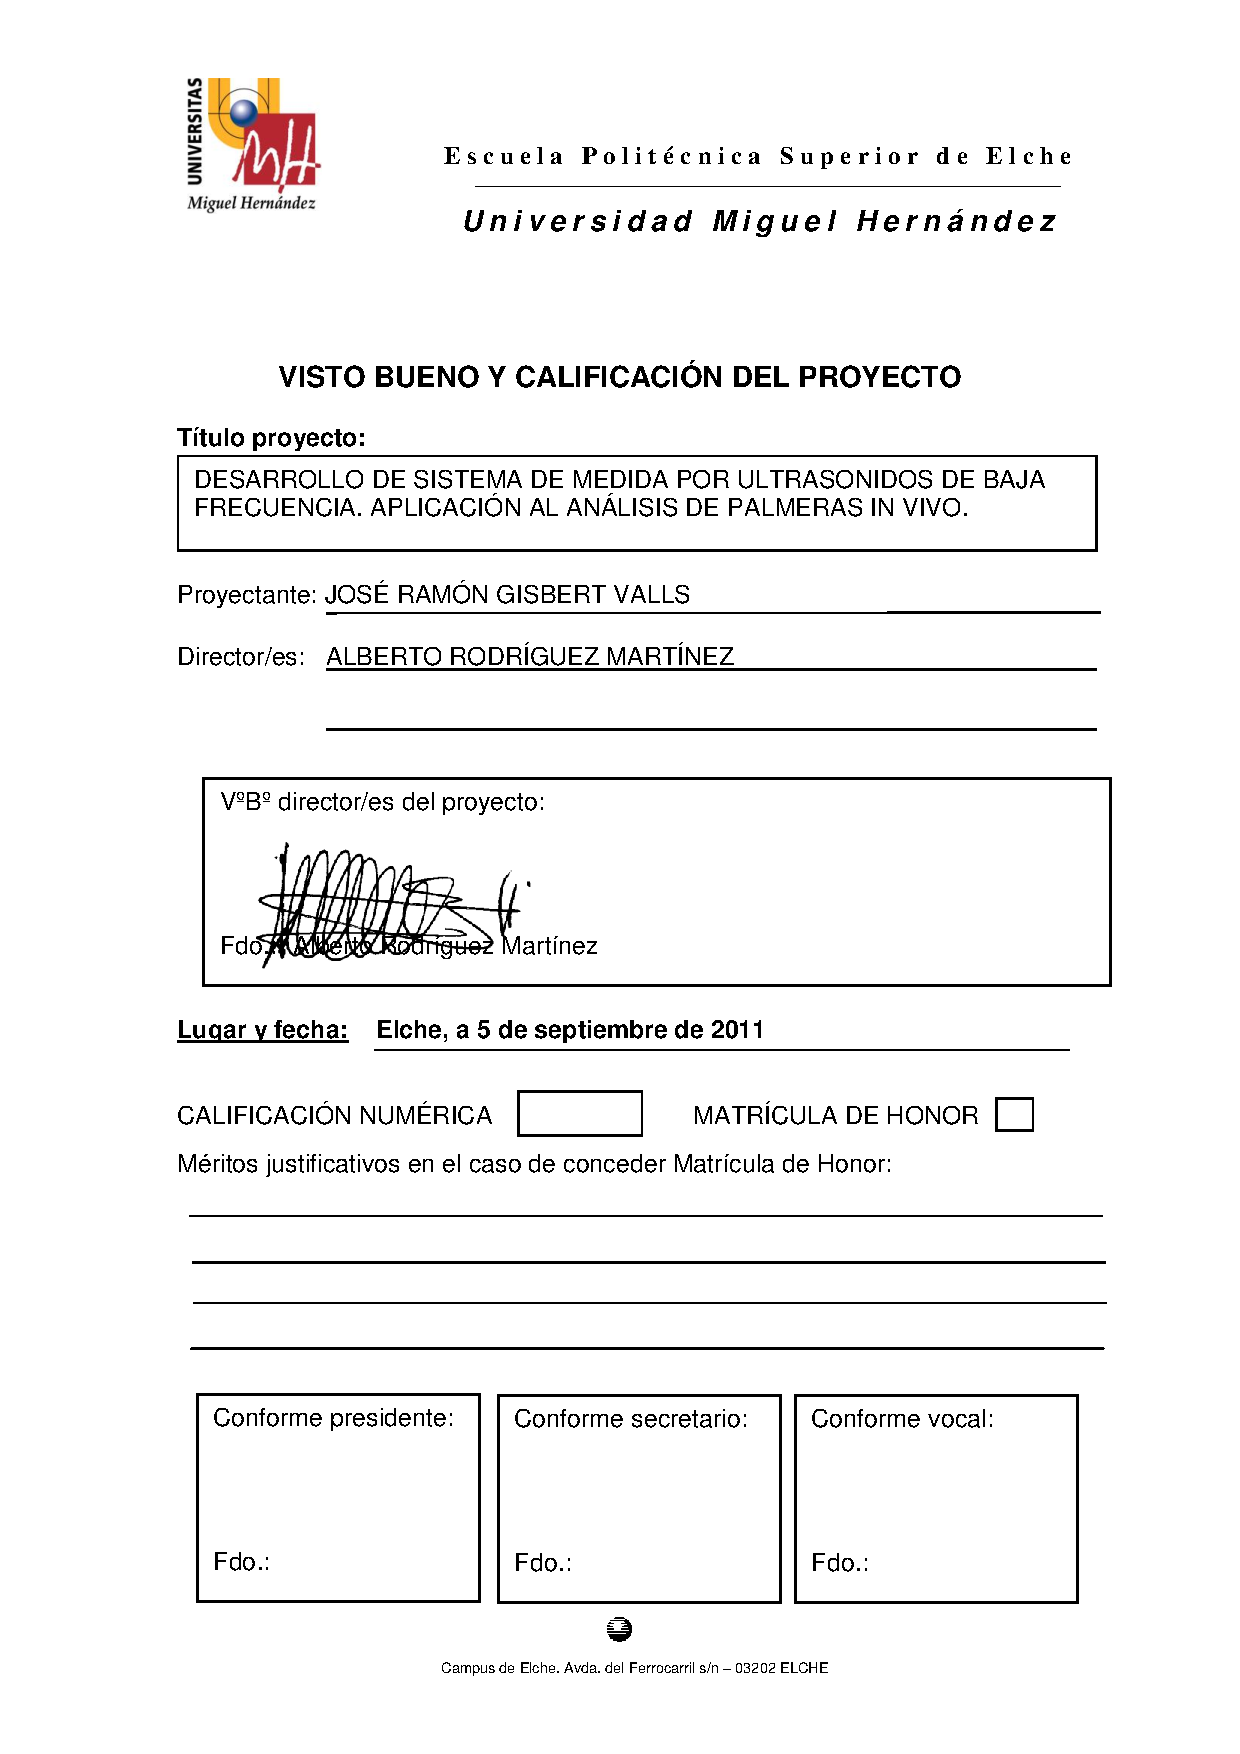
\includepdf[pages=-]{acta.pdf}


\pagestyle{Number}						% fancyhdr

\frontmatter

\tableofcontents
\listoftables
\listoffigures
\chapter{Pr�logo}

\subsubsection{Justificaci�n}

\paragraph{Ensayos no destructivos con ultrasonidos}

Es en la pr�ctica habitual en la actualidad emplear los \emph{ensayos no destructivos} (\psig{end}) en controles de calidad efectuados en la industria de manufactura de materiales, principalmente de metales y de compuestos para la construcci�n. Este tipo de ensayos garantizan ---demostrada su efectividad en este tipo de aplicaciones--- la ausencia de defectos internos como fisuras y de otras imperfecciones como alteraciones en la composici�n del producto, que de no superar controles semejantes pueden pasar inadvertidos. Realizando estos controles se impide la salida al mercado de partidas de producto defectuosas que pudiesen comprometer la calidad de productos finales. En este sentido comprobar el estado de un material resulta en un ejercicio de responsabilidad puesto que muchos de los materiales que proceden de esta industria se destinan a la construcci�n de edificios o de medios de transporte como barcos y aviones. De ah� la necesidad de aplicar en los controles de calidad m�todos que proporcionen resultados efectivos y confiables como lo son los obtenidos con los \sig{end}.\par
La ventajas que presentan los ensayos no destructivos frente a otro tipo de ensayos, no s�lo se limitan al hecho de que no es necesario sacrificar parte de la producci�n para evaluar el producto, si no que tambi�n incluyen una evaluaci�n continua y uniforme del material. Esto redunda en materiales de gran calidad cuyas propiedades se mantiene invariables uniformemente a lo largo del producto. Adem�s, otra ventaja de los \sig{end} es que es posible realizar de nuevo el ensayo una vez el producto final se ha terminado o en posteriores revisiones ya que no causa ning�n da�o en el material. Por �ltimo, cabe destacar que los controles de calidad mediante \sig{end} pueden efectuarse durante el mismo proceso de fabricaci�n de forma automatizada lo que supone una reducci�n en los costes.\par
Por su parte, el uso de ultrasonidos en \sig{end} est� muy extendido, esto es parcialmente debido a los precisos resultados que proporcionan los \emph{ensayos no destructivos mediante ultrasonidos} (\psig{endus}). Empleando transductores de alta frecuencia y gran ancho de banda es posible distinguir defectos en el material de tama�o muy peque�o de forma inequ�voca. A esto debe sum�rsele la sencillez con la que se aplican los \sig{endus} y las ventajas de emplear transductores de peque�o volumen que permiten trabajar con materiales de formas intrincadas e irregulares.\par
Recientemente se est�n empleando los \sig{endus} en campos experimentales con el prop�sito de detectar la presencia de anomal�as en materiales procedentes de la naturaleza. En estos experimentos el procedimiento a seguir es conforme al uso de los controles de calidad que se practican en el �mbito industrial. Conviene, sin embargo, diferenciar el tipo de medio en el que los ensayos son aplicados. Los ensayos realizados habitualmente a nivel industrial eval�an materiales sint�ticos, bien conocidos, mientras que en su lugar, los ensayos experimentales contemplan materiales org�nicos heterog�neos como es en este caso la madera. Es por ello que la eficacia de los \sig{endus} aplicados sobre materiales org�nicos no est� todav�a demostrada.\par
De la singularidad del material el inter�s de las pruebas, inter�s que se ve reforzado por el hecho de que la madera es un medio <<vivo>>, que cambia de muestra a muestra, las condiciones del ensayo var�an incluso para una misma muestra. Es, por tanto, el uso \sig{endus} para la detecci�n de defectos en madera de palmera un tema de inter�s, de actualidad y muy atractivo, hacia el cual orientar el desarrollo de un proyecto fin de carrera.


\paragraph{Tratamiento digital de se�ales}

El tratamiento digital de se�ales es una de las disciplinas fundamentales que abarca la ingenier�a de telecomunicaciones. Pese a los inconvenientes inherentes al uso de circuiter�a digital (derivados del muestreo y de la operaci�n de cuantificaci�n principalmente) el procesado digital de se�ales ha demostrado ser una herramienta �til y vers�til.\par
Esa versatilidad se sigue de la capacidad del hardware digital de ser programado, o lo que es lo mismo la capacidad de un circuito de alterar su funcionamiento y proporcionar varias funciones de acuerdo con una configuraci�n por software. Virtud que sumada al reciente desarrollo de las tecnolog�as digitales ha propiciado su explotaci�n y el uso extensivo de aplicaciones basadas en circuiter�a digital.\par
La configuraci�n de un sistema digital de medida a partir de una tarjeta de adquisici�n digital, un ordenador y una suite de software matem�tico supone una oportunidad para comprender aspectos del funcionamiento de los sistemas digitales dif�ciles de observar en la teor�a.


\subsubsection{Objetivos del proyecto fin de carrera}\label{sec:goals}

Inicialmente este proyecto persigue completar dos objetivos distintos: la implementaci�n de un sistema de medida a partir de una tarjeta de adquisici�n con interfaz \sig{pci}; y la evaluaci�n de los \sig{endus} como m�todo para la detecci�n de defectos en madera de palmera.\par
Por un lado, se ha llevado a cabo la puesta en funcionamiento de un sistema de medida con el que es posible obtener un conjunto de par�metros de una determinada se�al. Permite observar la forma que presenta la se�al en cada instante, la forma del espectro de la se�al cuando se enmarca en una ventana de una determinada duraci�n temporal, valores instant�neos y valores medios en un determinado intervalo.\par
Por otro lado, se han llevado a cabo una serie de pruebas experimentales en madera de palmera, empleando para ello se�ales ultras�nicas generadas por un transductor, de forma similar a como se hace en los \sig{endus} de car�cter industrial. Posteriormente las muestras se han procesado para averiguar a partir de los datos que informaci�n sobre el medio ---presencia de fisuras internas, presencia de agua en distintos niveles dependiendo de la altura en la que se realiza la prueba o del estado de salud del esp�cimen, o en general cualquier otra informaci�n de utilidad--- puede extraerse en este tipo de ensayos.\par
Existe una relaci�n visible entre ambos objetivos, la pretensi�n inicial consiste en emplear el sistema de medida digital en la realizaci�n de las pruebas. No obstante, pese a todo, durante el transcurso del proyecto ambos objetivos se tratan por separado. Finalmente, la imposibilidad de realizar las pruebas experimentales con el sistema confeccionado (por motivos que se ver�n m�s adelante) ha conducido al uso de un sistema de medida alternativo. Es por este motivo por el cual resulta comprensible la divisi�n de este documento en dos partes, una por cada objetivo diferenciado.


\subsubsection{Estructura del documento}

Como se ha mencionado al terminar el apartado anterior, el presente documento consta de dos partes. El contenido se ha distribuido en dos partes ordenadas como sigue: en primer lugar se aborda la configuraci�n del sistema digital de medida; para m�s tarde tratar la teor�a que concierne a los \sig{endus} y presentar los resultados obtenidos. Esta divisi�n del texto no es, sin embargo, natural por completo, puesto que para llevar a cabo el proceso de dise�o previo a la implementaci�n del sistema de medida es necesario haber reunido previamente un determinado conocimiento en materia de \sig{endus}. Pese a todo, es razonable considerar que la implementaci�n del sistema de medida debe tener lugar antes de la realizaci�n de las pruebas ---como ha ocurrido efectivamente--- y de ah� la elecci�n de este orden.\par
La primera parte se divide a su vez en cuatro cap�tulos: subsistema de interacci�n con el medio f�sico; subsistema de adquisici�n; subsistema de control y presentaci�n; y resultados, conclusiones y l�neas futuras de trabajo. Incluyendo una introducci�n previa a esta parte de la memoria. Los tres primeros cap�tulos responden a una divisi�n funcional del sistema de medida que se explica con detalle en la introducci�n.

\begin{description}
	\item[Primer cap�tulo] El primer subsistema interact�a directamente con el medio f�sico, comprende el transmisor de ultrasonidos, el receptor y las etapas de acondicionamiento que los acompa�an. El primer cap�tulo resume las principales caracter�sticas de estos tres elementos y realiza un recorrido por el proceso de dise�o de este subsistema.
	\item[Segundo cap�tulo] El subsistema intermedio transforma la se�al anal�gica que le es entregada por la secci�n de recepci�n en una se�al digital. El n�cleo y el todo de este subsistema es la tarjeta de adquisici�n. El segundo cap�tulo repasa las caracter�sticas t�cnicas clave de este dispositivo, realiza una descripci�n funcional del mismo y reproduce los consejos que el fabricante proporciona en el manual de usuario para su uso correcto.
	\item[Tercer cap�tulo] El �ltimo de los subsistemas act�a como interfaz entre el supervisor y el sistema de medida. Es el subsistema de control y presentaci�n. En el tercer cap�tulo se hace hincapi� en el dise�o conceptual de este subsistema y se proporcionan una serie de detalles t�cnicos en relaci�n con el entorno de programaci�n en el que se ha desarrollado.
	\item[Cuarto cap�tulo] En el �ltimo de los cap�tulos de la primera parte se exponen las conclusiones extra�das tras poner a prueba el sistema de medida ya terminado. Se comentan posteriormente l�neas futuras de trabajo que persiguen mejorar la funcionalidad del sistema de medida.
\end{description}

La segunda parte est� dividida en tres cap�tulos: fundamentos te�ricos de los \sig{endus}, descripci�n del medio, resultados y conclusiones.

\begin{description}
	\item[Quinto cap�tulo] En el primer cap�tulo se describen de forma superficial los distintos elementos que intervienen en un \sig{endus} desde un punto de vista te�rico. De las distintas t�cnicas existentes para combatir el ruido estructural se dan detalles sobre las t�cnicas de procesado por partici�n del espectro que son las utilizadas en este proyecto.
% 	\item[Segundo cap�tulo] El segundo cap�tulo trata sobre el medio en el que se realizan las pruebas experimentales, la madera de palmera. Se proporciona una descripci�n te�rica del material de acuerdo con la documentaci�n consultada. Se caracteriza el material para un posterior an�lisis de los resultados encontrados en las pruebas experimentales.
	\item[Sexto cap�tulo] El �ltimo cap�tulo recoge los resultados extra�dos de las pruebas en forma de grafos y tablas comentados. Despu�s se dan las conclusiones a las que se ha llegado a partir de estos resultados y finalmente se realizan una serie de comentarios sobre nuevas l�neas de investigaci�n que pueden seguirse de este proyecto
\end{description}

% Un sistema de medida es cualquier instrumento formado por m�s de un elemento que permite a quien lo usa evaluar una determinada propiedad de un objeto, medio o evento. Para una definici�n m�s rigurosa de un sistema electr�nico de medida puede optarse por la encontrada en \cite{pallas2003sas}, y dice lo siguiente:
% 
% {\small\begin{quotation}
% 	Se denomina sistema a la combinaci�n de dos o m�s elementos, subconjuntos y partes necesarias para realizar una o varias funciones. En los sistemas de medida, esta funci�n es la asignaci�n objetiva y emp�rica de un n�mero a una propiedad o cualidad de un objeto o evento, de tal forma que la describa.
% \end{quotation}}
% 
% Un sistema de medida digital est� constituido habitualmente por los elementos mostrados en el esquema de la \cref{fig:digmeasstm}. Pueden agruparse estos elementos seg�n la funci�n que desempe�an en el sistema, si se hace de ese modo se encuentran tres subsistemas: un subsistema para la interacci�n con el medio f�sico, un subsistema de adquisici�n, y un subsistema de control y presentaci�n. Puede observarse entonces el sistema como una pila de capas superpuestas, en el que cada capa provee de servicio a la capa inmediatamente superior y abstrae las capas inferiores, en cada una de las capas se situar�a cada uno de los subsistemas propuestos. De ese modo cada subsistema puede estudiarse por separado con independencia de los dem�s, as� se ha hecho en esta memoria. Consecuentemente cada subsistema da lugar a cada uno de los tres cap�tulos que siguen a esta introducci�n.\par
% 
% \begin{figure}
% 	\begin{center}
% 		\includegraphics{gis-pfc-part1-01.mps}
% 	\end{center}
% 	\caption[Sistema digital de medida]{Distintos elementos funcionales que conforman el sistema digital de medida.}
% 	\label{fig:digmeasstm}
% \end{figure}
% 
% Si se define una jerarqu�a en la que el nivel m�s bajo es aquel ocupado por los elementos en contacto directo con el medio, y se tiene como nivel m�s alto aquel en el que se encuentran los elementos que interact�an con el supervisor, entonces los niveles ordenados de inferior a superior en la jerarqu�a establecida se encuentran ocupados por los subsistemas precisados anteriormente del siguiente modo: subsistema para la interacci�n con el medio, subsistema de adquisici�n, y subsistema de control y presentaci�n. El orden en el que se han dispuesto los cap�tulos que tratan acerca de la configuraci�n del sistema digital de medida, los tres primeros cap�tulos, coincide con el orden que guardan los distintos subsistemas en esta jerarqu�a. De ese modo en estos tres cap�tulos se encuentra el siguiente contenido:
% 
% \begin{enumerate}
% 	\item En primer lugar, el primer cap�tulo trata sobre el subsistema que se encuentra en el estrato m�s bajo de la jerarqu�a, el subsistema para la interacci�n con el medio. Este subsistema comprende ---como se ha dicho en el pr�logo--- el sensor, el actuador y los circuitos acondicionadores que los siguen. Estos son los elementos fundamentales de un sistema electr�nico de medida, con ellos puede implementarse el sistema de medida m�s b�sico y sin ellos no existen los sistemas de medida.\par
% 	\item El segundo cap�tulo abarca el subsistema de adquisici�n. Este subsistema es el encargado de digitalizar la se�al anal�gica que provee el subsistema para la interacci�n en el medio y administrar la se�al digital resultante al bloque de presentaci�n para que pueda procesarla. Es un subsistema propio y distintivo de los sistemas digitales de medida, ya que s�lo esta presente en este tipo de sistemas. En este caso se encuentra constituido por un �nico elemento, la tarjeta de adquisici�n.
% 	\item El �ltimo de los subsistemas, el subsistema de m�s alto nivel, el subsistema de control y presentaci�n, se estudia en el tercer cap�tulo. Este subsistema interviene como interfaz entre el usuario administrador y el resto de capas (el sistema de medida). Como tal es su funci�n traducir la se�al digital que recibe de capas inferiores en informaci�n �til para el usuario, en informaci�n que �ste pueda interpretar. Por otro lado es su funci�n tambi�n gestionar el sistema de medida por medio de los comandos que le env�a el supervisor, en otras palabras, el subsistema de control es el encargado de ejecutar las �rdenes del administrador del sistema.\par
% \end{enumerate}



\mainmatter

\part[Implementación del sistema digital de medida] %
{Diseño e implementación del sistema digital de medida}
\pagestyle{number}						% fancyhdr
\chapter*{Introducción}

\section*{Organización de la primera parte}

Como se ha dicho, el presente documento consta de dos partes. El contenido
se ha distribuido en dos partes ordenadas como sigue: en primer lugar se
aborda la configuración del sistema digital de medida; para más tarde
tratar la teoría en la que se sustentan los \sig{endus} y presentar los
resultados obtenidos. Esta división del texto no es, sin embargo, del todo
natural, puesto que para llevar a cabo el proceso de diseño previo a la
implementación del sistema de medida es necesario haber reunido previamente
un determinado conocimiento en materia de \sig{endus}. Pese a todo, es
razonable considerar que la implementación del sistema de medida debe tener
lugar antes de la realización de las pruebas ---como ha ocurrido
efectivamente--- y de ahí la elección de este orden.

La primera parte se divide a su vez en cuatro capítulos: subsistema de
interacción con el medio físico; subsistema de adquisición; subsistema de
control y presentación; y resultados, conclusiones y líneas futuras de
trabajo. Los tres primeros capítulos responden a una división funcional del
sistema de medida que se explica con detalle en el siguiente apartado, más
adelante en esta misma introducción.


\begin{description}
	\item[Primer capítulo] El primer subsistema interactúa directamente
		con el medio físico, comprende el transmisor de
		ultrasonidos, el receptor y las etapas de acondicionamiento
		que los acompañan. El primer capítulo resume las
		principales características de estos tres elementos y
		realiza un recorrido por el proceso de diseño de este
		subsistema.
	\item[Segundo capítulo] El subsistema intermedio transforma la
		señal analógica que le es entregada por la sección de
		recepción en una señal digital.  El núcleo y el todo de
		este subsistema es la tarjeta de adquisición. El segundo
		capítulo repasa las características técnicas clave de este
		dispositivo, realiza una descripción funcional del mismo y
		reproduce los consejos que el fabricante proporciona en el
		manual de usuario para su uso correcto.
	\item[Tercer capítulo] El último de los subsistemas actúa como
		interfaz entre el supervisor y el sistema de medida. Es el
		subsistema de control y presentación. En el tercer capítulo
		se hace hincapié en el diseño conceptual de este subsistema
		y se proporcionan una serie de detalles técnicos en
		relación con el entorno de programación en el que se ha
		desarrollado.
	\item[Cuarto capítulo] En el último de los capítulos de la primera
		parte se exponen las conclusiones extraídas tras poner a
		prueba el sistema de medida ya terminado. Se comentan
		posteriormente líneas futuras de trabajo que persiguen
		mejorar la funcionalidad del sistema de medida.
\end{description}


\section*{El sistema digital de medida}

Un sistema de medida es cualquier instrumento formado por más de un
elemento que permite a quien lo usa evaluar una determinada propiedad de un
objeto, medio o evento. Para una definición más rigurosa de un sistema
electrónico de medida puede optarse por la encontrada en
\cite{pallas2004sas}, y dice lo siguiente:

{\small\begin{quotation}
	Se denomina sistema a la combinación de dos o más elementos,
	subconjuntos y partes necesarias para realizar una o varias
	funciones. En los sistemas de medida, esta función es la asignación
	objetiva y empírica de un número a una propiedad o cualidad de un
	objeto o evento, de tal forma que la describa.
\end{quotation}}

Un sistema de medida digital está constituido habitualmente por los
elementos mostrados en el esquema de la \cref{fig:digmeasstm}. Pueden
agruparse estos elementos según la función que desempeñan en el sistema, si
se hace de ese modo se encuentran tres subsistemas: un subsistema para la
interacción con el medio físico, un subsistema de adquisición, y un
subsistema de control y presentación. Puede observarse entonces el sistema
como una pila de capas superpuestas, en el que cada capa provee de servicio
a la capa inmediatamente superior y abstrae las capas inferiores, en cada
una de las capas se situaría cada uno de los subsistemas propuestos. De ese
modo cada subsistema puede estudiarse por separado con independencia de los
demás, así se ha hecho en esta memoria. La división funcional del sistema
de medida que se ha propuesto aquí se refleja en la organización del
documento de modo que cada uno de los capítulos de la primera parte trata
únicamente sobre un subsistema y los elementos que forman parte del mismo.

\begin{figure}
	\begin{center}
		\includegraphics{gis-pfc-part1-01.pdf}
	\end{center}
	\captionsetup{listformat=romanos, labelformat=romanos}
	\caption[Sistema de medida digital]{Distintos elementos funcionales
	que conforman el sistema digital de medida.}
	\label{fig:digmeasstm}
\end{figure}

\llongpage{}
Si se define una jerarquía en la que el nivel más bajo es aquel ocupado por
los elementos en contacto directo con el medio, y se tiene como nivel más
alto aquel en el que se encuentran los elementos que interactúan con el
supervisor, entonces los niveles ordenados de inferior a superior en la
jerarquía establecida se encuentran ocupados por los subsistemas precisados
anteriormente del siguiente modo: subsistema para la interacción con el
medio, subsistema de adquisición, y subsistema de control y presentación.
El orden en el que se han dispuesto los capítulos que tratan acerca de la
configuración del sistema digital de medida, los tres primeros capítulos,
coincide con el orden que guardan los distintos subsistemas en esta
jerarquía.

\pagestyle{body}						% fancyhdr
\chapter{Tarjeta de adquisici�n de se�ales}

Uno de los objetivos que persigue este proyecto desde el comienzo es constituir un sistema de adquisici�n y procesado de se�ales. La idea es utilizar el sistema a la hora de afrontar la segunda parte del proyecto, o parte principal podr�a decirse, la experimentaci�n con palmeras, con sus troncos y madera, para evaluar la efectividad de los ensayos no destructivos, de esos que emplean los ultrasonidos como herramienta de exploraci�n. Es esta secci�n del documento la que se ocupa en la materia de retratar la experiencia de componer un instrumento que muestrea una se�al anal�gica y proporciona una versi�n digital de la misma, forma que permite su posterior procesado, almacenamiento y representaci�n.\par
La tarjeta \kpci{} adquiere un gran protagonismo en el sistema de adquisici�n y procesado, constituye la base del mismo. Este dispositivo constituye el fundamento a partir del cual se construye el resto del sistema de medida, incluyendo no s�lo la etapa de adquisici�n si no tambi�n las de acondicionamiento y detecci�n, parte de sus capacidades las hereda el sistema, sus limitaciones deben tenerse en cuenta en la fase de dise�o, de ah� la importancia de estudiar a conciencia su comportamiento. Adem�s, la \kpci{}, disponer de ella, es una de las razones principales por las que se ha optado por desarrollar un sistema de adquisici�n propio, de prop�sito, sin tener en cuenta la principal raz�n, como es obvio, contar con un sistema dise�ado a medida.\par
Resulta primordial pues conocer las caracter�sticas de una pieza tan importante del conjunto, de hecho es el primer paso que se toma en la ejecuci�n del proyecto, estudiar el aparato y averiguar hasta d�nde alcanzan sus posibilidades. En la memoria del proyecto queda plasmado el inter�s que suscita la tarjeta desde un punto de vista pr�ctico en relaci�n con la s�ntesis de un sistema de adquisici�n y procesado puesto que se dedica un cap�tulo completo a tratar en clave t�cnica y de forma resumida c�mo funciona la tarjeta y cu�les son sus propiedades m�s destacadas.


\section{Caracter�sticas t�cnicas del hardware}\label{sec:technical}

La tarjeta \kpci{} puede emplearse para la adquisici�n y conversi�n de se�ales anal�gicas en se�ales digitales, para sintetizar se�ales anal�gicas a partir de se�ales digitales previamente generadas o almacenadas, o ---gracias a sus 32 puertos digitales de prop�sito general--- trabajar con se�ales digitales.\par
El primer bloque del sistema electr�nico de medida propuesto, es decir el sistema de adquisici�n y procesado de se�ales, tan s�lo requiere de la funci�n de adquisici�n anal�gica de la tarjeta. Por ello, de entre todas las caracter�sticas del dispositivo, se ha cre�do conveniente resumir a continuaci�n aquellas que tienen relaci�n directa con dicha funci�n. Para obtener informaci�n detallada sobre la relaci�n que estos atributos guardan con el proceso de adquisici�n de se�ales anal�gicas en la tarjeta \kpci{}, v�ase la \vref{sec:funcdesc}.

\begin{itemize}
	\item El m�dulo de adquisici�n anal�gica dispone de 16 puertos f�sicos.
	\item La impedancia de entrada equivalente de cada puerto es aproximadamente igual a una capacidad de 200 pF en serie con una resistencia de valor inferior, pero aproximadamente igual, a 1 k$\Omega$.
	\item En condiciones �ptimas, es posible conseguir un rendimiento m�ximo de 100 KS/s (cien mil operaciones de conversi�n por segundo). Este valor est� sujeto a un error relativo del $0.02\%$.
	\item La resoluci�n del conversor anal�gico digital es de 16 bits por muestra. El rango de amplitudes en el que opera depende de como est� configurado el modo de adquisici�n. Puede ir de 0 V a 10 V si el modo de adquisici�n es unipolar, o de -10 V a 10 V si es bipolar.
	\item La cola de muestreo tiene capacidad para hasta 256 canales distintos. Cada uno de los cuales puede configurarse independientemente en t�rminos de ganancia, frecuencia de muestreo, modo de adquisici�n o modo de terminaci�n.
	\item La ganancia, responsable en parte de la resoluci�n con la que se cuantifica las muestras, puede tomar cada ciclo de reloj uno de entre 16 valores posibles (v�ase el \vref{tab:acqmodes}).
\end{itemize}


\section{Descripci�n funcional}\label{sec:funcdesc}

Es necesario programar el comportamiento de la tarjeta de adquisici�n antes de ponerla en funcionamiento. Desde la cola de muestreo se controlan los principales aspectos del proceso de adquisici�n, como por ejemplo, en que instantes se encuentra activo.\par
La cola de muestreo, como su propio nombre indica, es una estructura de datos ordenada. Se encuentra almacenada en una memoria \sig{ram} de 256 entradas que forma parte del hardware de la tarjeta. En el \vref{tab:queue} puede verse una representaci�n de un ejemplo de la cola de muestreo.\par

\begin{table}
	\centering
	\begin{threeparttable}
	\begin{tabular}{lccccccccc}
		\toprule
		Posici�n en la cola & 1 & 2 & 3 & 4 %
		& \multicolumn{2}{c}{$\cdots$} & 254 & 255 & 256 \\
		\midrule
		N�mero de canal & 15 & 15 & 02 & 02 %
		& \multicolumn{2}{c}{$\cdots$} & 17 & 13 & 01 \\
		N�mero de puerto\tnote{a, b} & 07 & 07 & 11 & 11 %
		& \multicolumn{2}{c}{$\cdots$} & 07 & 09 & 01 \\
		Ganancia & 1 & 1 & 40 & 40 %
		& \multicolumn{2}{c}{$\cdots$} & 200 & 8 & 80 \\
		Modo de adquisici�n\tnote{c} & $\pm$ & $\pm$ & $+$ & $+$ %
		& \multicolumn{2}{c}{$\cdots$} & $\pm$ & $+$ & $\pm$ \\
		Modo de terminaci�n\tnote{d} & \sig{d} & \sig{d} & \sig{m} %
		& \sig{m} & \multicolumn{2}{c}{$\cdots$} & \sig{d} & \sig{m} %
		& \sig{m} \\
		\bottomrule
	\end{tabular}
	\begin{TableNotes}
		\tnotetext{a}{Si el canal es diferencial el n�mero de puerto identifica un par de puertos. Un canal diferencial no puede estar asociado a un n�mero de puerto superior a 07.}
		\tnotetext{b}{Dos canales pueden estar relacionados con los mismos puertos f�sicos.}
		\tnotetext{c}{Se define: configuraci�n bipolar ($\pm$); configuraci�n unipolar ($+$)}
		\tnotetext{d}{Se define: canal diferencial (\sig{d}); canal monoterminal (\sig{m})}
	\end{TableNotes}
	\end{threeparttable}
	\caption{Ejemplo de cola de muestreo}
	\label{tab:queue}
\end{table}

Cada entrada en la memoria \sig{ram} se identifica con una posici�n en la cola. Las posiciones en la cola pueden encontrarse vac�as o estar ocupadas por un canal. Varias posiciones en la cola, consecutivas o no, pueden estar ocupadas por un mismo canal. Por tanto, la cola puede estar ocupada, como m�ximo, por 256 canales independientes.\par
Las posiciones ocupadas contienen informaci�n correspondiente al canal y a los atributos asociados a este. Un canal es una entidad l�gica que relaciona un puerto f�sico con un b�ffer de informaci�n y una serie de atributos. Durante el proceso de adquisici�n un puntero recorre las distintas posiciones de la cola, una a una y en orden. El canal activo, aquel que ocupa la posici�n a la que apunta el puntero en cada ciclo de reloj, determina tres cosas:

\begin{itemize}
	\item De qu� puerto debe proceder la se�al anal�gica\footnote{Por convenio se ha elegido hablar de una sola se�al que entra al amplificador. Si se ha hecho esta elecci�n, es porque si bien al amplificador pueden entrar una o dos se�ales simult�neamente, esto no supone otra diferencia para el proceso que la expuesta en el \vref{subsubsec:termmodes}. Es por ello, y para mantener la claridad, que se ha omitido esta posibilidad.} que llega al amplificador de instrumentaci�n interno de la tarjeta.
	\item D�nde, en qu� b�ffer, debe almacenarse el valor resultante de muestrear y cuantificar esta se�al.
	\item Por �ltimo, los atributos asociados al canal: ganancia, modo de adquisici�n y modo de terminaci�n; indican, respectivamente: cual debe ser la ganancia del amplificador de instrumentaci�n, cual debe ser el rango de trabajo del conversor anal�gico digital, y que se debe conectar a los terminales de entrada del amplificador de instrumentaci�n. Se da m�s informaci�n al respecto en apartados subsiguientes.% la polaridad de las muestras y el n�mero de terminales de entrada, uno o dos dependiendo de si la adquisici�n es diferencial o no, durante el ciclo actual.
\end{itemize}

Para concluir el apartado cabe remarcar lo siguiente. Es posible inferir dos cosas de esta mec�nica de funcionamiento basada en la cola. Una de ellas es que el proceso de adquisici�n afecta a una sola se�al cada vez. Y la segunda, que la frecuencia de muestreo ligada a un canal depende de dos factores, de la velocidad de la se�al de reloj, y de la cantidad de veces que un canal aparece repetido en la cola.


\subsection{M�todos de entrada}

La \kpci{} permite dos modos de adquisici�n y dos modos de terminaci�n. Aprender a diferenciar cuando es oportuno seleccionar entre cada uno de ellos beneficiar� la calidad de la se�al digital resultante.


\subsubsection{Modos de adquisici�n}
Una se�al es bipolar cuando toma valores positivos y negativos. Por el contrario, se distingue a las se�ales unipolares porque todos sus valores mantienen la misma polaridad, ya sea �sta positiva o negativa. Para cada canal, debe configurarse el modo de adquisici�n como bipolar o unipolar\footnote{La tarjeta \kpci{} s�lo admite se�ales unipolares de polaridad positiva.} atendiendo a la se�al de inter�s.\par
Si se sabe a ciencia cierta que la se�al de entrada es unipolar debe emplearse el modo de adquisici�n unipolar. De ese modo, se duplica la resoluci�n del conversor anal�gico digital.

\begin{table}
	\centering
	\begin{tabular}{>{\raggedleft}p{1.2cm}d{5.2}d{3.1}+d{3.1}}
		\toprule
		& \multicolumn{2}{c}{Bipolar} & \multicolumn{2}{c}{Unipolar} \\
		\cmidrule(r){2-3}\cmidrule(l){4-5}
		\multicolumn{1}{c}{Ganancia}
		& \multicolumn{1}{c}{Rango ($\pm\text{V}$)} %
		& \multicolumn{1}{c}{Precisi�n ($\mu\text{V}$)} %
		& \multicolumn{1}{c}{Rango (V)} %
		& \multicolumn{1}{c}{Precisi�n ($\mu\text{V}$)} \\
		\midrule
		1 & 10,0 & 305 & 0/$10,0$ & 153 \\
		2 & 5,0 & 153 & 0/$5,0$ & 76 \\
		4 & 2,5 & 76 & 0/$2,5$ & 38 \\
		8 & 1,25 & 38 & 0/$1,25$ & 19 \\
		10 & 1,0 & 31 & 0/$1,0$ & 15 \\
		\\
		& \multicolumn{2}{c}{Bipolar} & \multicolumn{2}{c}{Unipolar} \\
		\cmidrule(r){2-3}\cmidrule(l){4-5}
		\multicolumn{1}{c}{Ganancia}
		& \multicolumn{1}{c}{Rango ($\pm\text{mV}$)} %
		& \multicolumn{1}{c}{Precisi�n ($\mu\text{V}$)} %
		& \multicolumn{1}{c}{Rango (mV)} %
		& \multicolumn{1}{c}{Precisi�n ($\mu\text{V}$)} \\
		\midrule
		20 & 500 & 15 & 0/500 & 7,6 \\
		40 & 250 & 7,6 & 0/250 & 3,8 \\
		80 & 125 & 3,8 & 0/125 & 1,9 \\
		100 & 100 & 3,1 & 0/100 & 1,5 \\
		200 & 50 & 1,5 & 0/50 & 0,8 \\
		400 & 25 & 0,8 & 0/25 & 0,4 \\
		800 & 12,5 & 0,4 & 0/$12,5$ & 0,2 \\
		\bottomrule
	\end{tabular}
	\caption{Relaci�n entre ganancia, rango de trabajo y resoluci�n seg�n el modo de adquisici�n}
	\label{tab:acqmodes}
\end{table}


\subsubsection{Modos de terminaci�n}\label{subsubsec:termmodes}

Internamente, la tarjeta \kpci{} emplea un amplificador de instrumentaci�n diferencial. En principio este hecho implicar�a que a cada canal se asociasen dos puertos f�sicos, uno por cada uno de los dos terminales de entrada del amplificador. No obstante, es posible configurar la tarjeta para que uno de los terminales del amplificador se conecte a masa. En ese caso, el terminal restante se conecta a un puerto f�sico. La \vref{fig:termmodes} muestra un ejemplo de esta configuraci�n.\par

\begin{figure}
	\begin{center}
		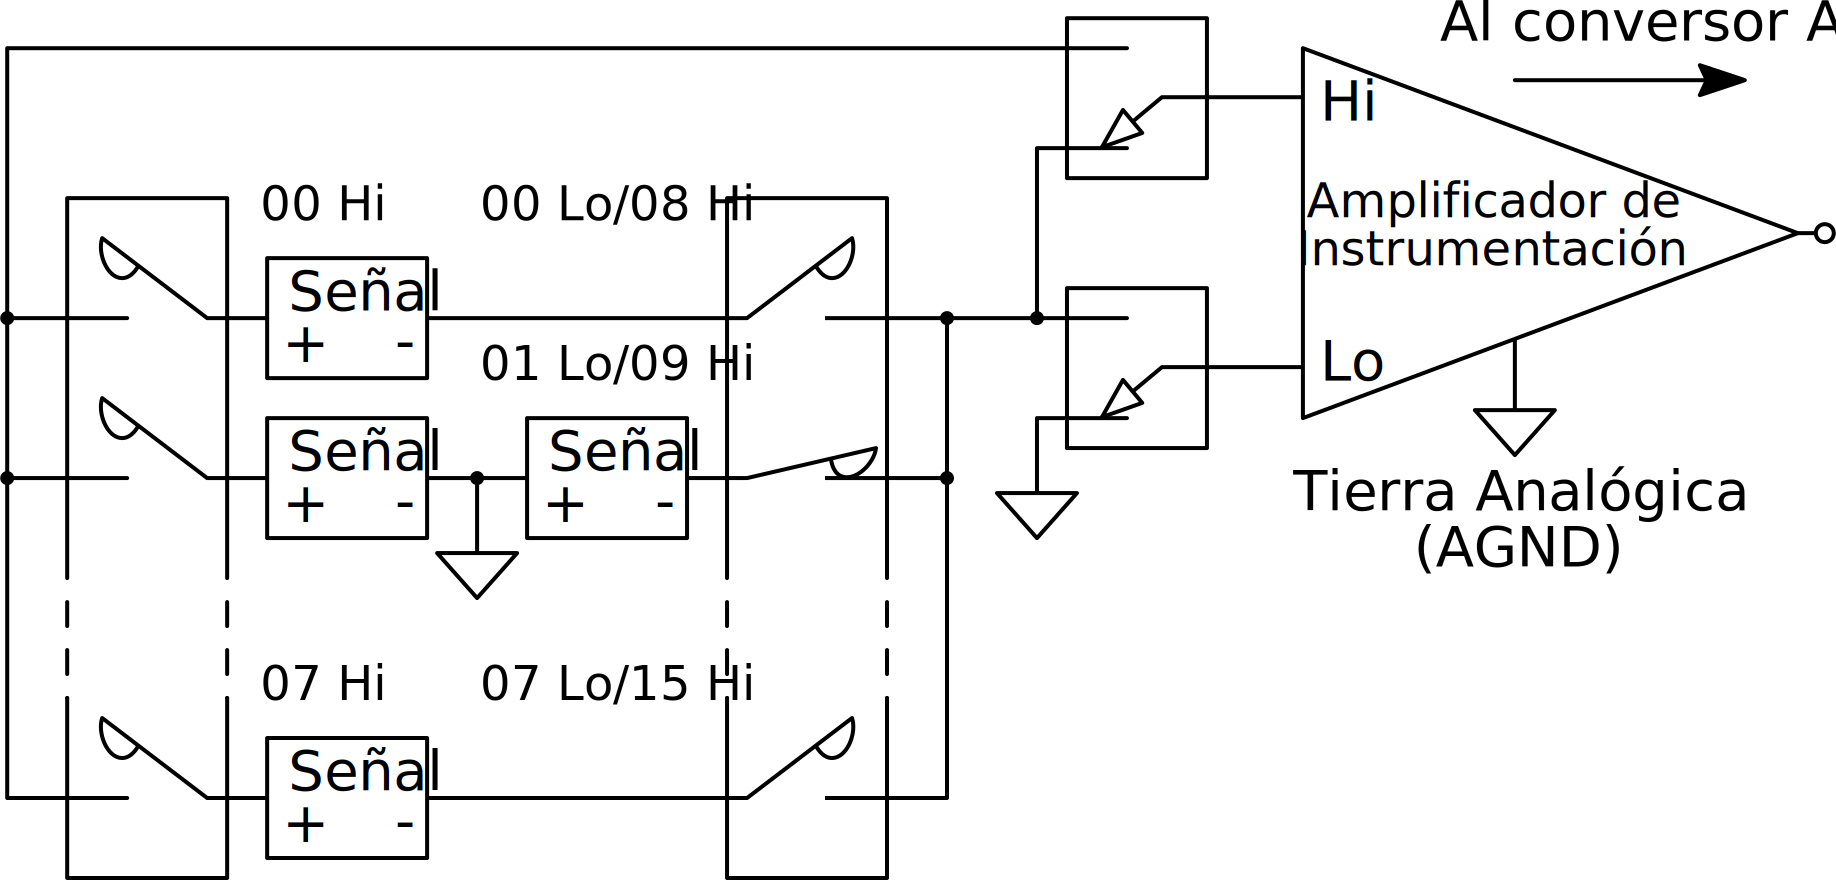
\includegraphics{gis-pfc-ch1-1.mps}
	\end{center}
	\caption[Ejemplo de configuraci�n de terminaci�n]{Figura que muestra el modo de terminaci�n sencillo. La entrada superior del amplificador de instrumentaci�n se conecta al puerto 9 y la entrada inferior se conecta a masa}
	\label{fig:termmodes}
\end{figure}

Para habilitar semejante configuraci�n, cabr�a pensar que es suficiente con modificar el atributo que controla el modo de terminaci�n del canal correspondiente. Al contrario de lo que pudiera parecer, el modo de terminaci�n es una propiedad que no es atribuible al canal, si no que se atribuye a un par de puertos\footnote{Aunque seg�n las especificaciones del fabricante es posible configurar cada par de puertos para que opere seg�n un modo de terminaci�n independiente del resto, el entorno de desarrollo utilizado durante el proyecto s�lo admite un modo de terminaci�n para el conjunto total de puertos (v. el \vref{subsec:environment}).}. En concreto, el modo de terminaci�n afecta a los pares de puertos compuestos por un primero de entre los puertos 0 y 7, y un segundo cuyo n�mero de puerto es igual al del primero m�s 8. De ah� que todos los canales relacionados con el mismo par de puertos deban estar configurados con el mismo modo de terminaci�n, una configuraci�n distinta no est� permitida.\par
Los dos modos de terminaci�n posibles se conocen como: diferencial, si es que la se�al que entra en cada terminal del amplificador procede de cada uno de los puertos del par; sencillo, en caso de que uno de los terminales de entrada del amplificador se conecte a la referencia de tensi�n. En este documento se llama canal diferencial a los canales cuyo modo de terminaci�n sea diferencial, y canal con un s�lo terminal o monoterminal a aquellos para los que el modo de terminaci�n es sencillo. \par
Las ventajas que presenta el uso de uno u otro tipo de canales son comprensibles. Emplear canales con un s�lo terminal permite aplicar el proceso de adquisici�n sobre un mayor n�mero de se�ales simult�neamente. Por el contrario, utilizar canales diferenciales redunda en una mayor inmunidad frente al ruido. Adem�s, los amplificadores diferenciales eliminan de forma inherente la componente en continua.\par


\subsection{Rendimiento}\label{subsec:throughput}

Se entiende como rendimiento la cantidad m�xima de operaciones de conversi�n que el dispositivo puede realizar por unidad de tiempo. Para que una de estas operaciones contribuya a la medida de rendimiento debe superar un requisito de precisi�n.\par
El rendimiento �ptimo de la tarjeta \kpci{} especificado por el fabricante es de cien mil operaciones por segundo (100 KS/s). No obstante se advierte, para obtener este nivel de rendimiento es necesario alimentar la tarjeta con una fuente de tensi�n ideal. Adem�s, es importante que exista adaptaci�n de impedancias entre el circuito de alimentaci�n y el puerto por el que se quiere introducir la se�al. A�n en estas condiciones el valor proporcionado por la casa Keithley est� sujeto a un error relativo m�ximo del $0.02\%$, el cual supone un error absoluto m�ximo de dos mil operaciones por segundo (2 KS/s).\par
Es bien sabido, a trav�s del teorema de Nyquist, que la frecuencia de muestreo con la que debe muestrearse una se�al anal�gica para que esta pueda ser recuperada a partir de la versi�n digital obtenida en el proceso de muestreo debe ser mayor o igual al doble de la mayor de las frecuencias con las que oscila la se�al original, siempre que esta sea peri�dica y se encuentre limitada en banda. No obstante, en la pr�ctica, para poder elaborar una representaci�n visual aceptable de se�ales que no se encuentren sujetas a tales limitaciones ---ancho de banda finito y periodicidad de la se�al--- la frecuencia de muestreo debe estar en torno a unas cinco veces el l�mite superior de frecuencias correspondiente a la se�al que desea representarse. Por este motivo el rendimiento del dispositivo de adquisici�n y por ende del sistema de adquisici�n y procesado que en �ste se sustenta es un factor limitante que determina la frecuencia de oscilaci�n m�xima de la se�ales con las que dicho sistema trabaja. En este caso, considerando el montaje propuesto para el desarrollo de los experimentos que ata�en a este proyecto, el rendimiento de la \kpci{} limita la frecuencia de operaci�n de los transductores empleados y, en consecuencia, la profundidad de penetraci�n de los pulsos ultras�nicos y, por consiguiente, el espesor m�ximo de las muestras empleadas en los experimentos. Esta relaci�n surge inequ�vocamente de las conclusiones que se extraen de los desarrollos llevados a cabo en este mismo documento en el \cref{subsec:field}, expuestas en parte en otro \nameref{subsec:quality}, el \vref{subsec:quality}.


\subsubsection[Factores limitantes del rendimiento]{Amplificador de instrumentaci�n y p�rdida del rendimiento}

El amplificador de instrumentaci�n interno de la \kpci{} es de ganancia variable. Es posible configurar una ganancia distinta para cada canal. El prop�sito del amplificador es permitir al usuario modificar la amplitud de la se�al que entra al conversor. La intenci�n que se persigue es conseguir que la conversi�n se enfoque en los detalles de la se�al que sean de mayor inter�s y se pierda la m�nima informaci�n posible. Todo ello a�n trabajando simult�neamente con m�ltiples se�ales cuyo rango de amplitudes es con frecuencia muy diferente.\par
La desventaja que presenta esta configuraci�n ---multiplexor, amplificador de instrumentaci�n, conversor--- es una p�rdida de rendimiento que se produce en situaciones determinadas a causa de la intervenci�n del amplificador en la operaci�n de adquisici�n.\par
Cada ciclo de reloj cambia el canal activo y debe cambiar, si es oportuno, la se�al que accede al amplificador. Este proceso no es inmediato. Tras conmutar el multiplexor que precede al amplificador, se da paso al puerto conveniente. No obstante, la se�al que recibe el amplificador presenta, hasta transcurrido un determinado periodo de tiempo, una componente residual de la se�al que se amplific� en el anterior ciclo de reloj. Transcurrido dicho periodo de tiempo la se�al que entra al amplificador se ve libre de esa componente residual y se corresponde �nicamente con la se�al que entrega el multiplexor, se dice que se ha fijado la se�al.\par
Y es as� como el amplificador es causa de p�rdida de rendimiento, por medio de las componentes residuales. Si la conversi�n se realiza antes de fijar la se�al, el conversor toma un valor de la se�al corrompido por la componente residual de la se�al precedente. Por tanto, la muestra resultante queda igualmente corrompida incluso hasta el punto de perder su validez. Las operaciones de conversi�n que tengan como resultado muestras inv�lidas s�lo contribuyen a falsear la medida de rendimiento, haciendo que parezca mayor de lo que en realidad es.\par
El fabricante da a entender que existe una soluci�n de dise�o que resuelve en parte el problema planteado por las componentes residuales. Esta soluci�n consiste en alargar de forma deliberada la duraci�n del ciclo de reloj, de esa forma se proporciona tiempo suficiente para fijar la se�al. Sin embargo, esta soluci�n presenta dos inconvenientes: no solventa el problema en la totalidad de los casos y es, asimismo, una forma de perder rendimiento. Lo cual conduce inevitablemente a una soluci�n de compromiso, alargar el ciclo de reloj lo suficiente para que en la mayor�a de los casos el efecto de las componentes residuales sobre la precisi�n de la conversi�n no invalide las muestras resultantes y se produzca, por tanto, una ca�da del rendimiento, sin que la duraci�n del nuevo ciclo contribuya por s� misma a una p�rdida notable de �ste.\par


\subsubsection{Optimizaci�n del rendimiento}

Como se ha visto, la inclusi�n del amplificador en el dise�o de la tarjeta es causa directa o indirecta de una p�rdida de rendimiento. La magnitud de esa ca�da en el rendimiento depende de la configuraci�n de la cola de muestreo y de la amplitud de la se�al una vez llega �sta al dispositivo de adquisici�n.

\begin{itemize}
	\item Las se�ales cuya tensi�n absoluta se encuentra por debajo de los 100 mV al llegar a la \kpci{} sufren en mayor medida las consecuencias del empleo de un amplificador en la operaci�n de conversi�n. En primer lugar la se�al tarda m�s en fijarse de modo que el rendimiento se reduce a la mitad en las mejores condiciones, de 100 KS/s pasa a 50 KS/s. Esto es debido a que, al ser la amplitud de la se�al y la del ruido comparables, especialmente despu�s de que �ste se vea reforzado por el efecto de las componentes residuales, se genera una mayor incertidumbre.\par
	Por otro lado las se�ales que requieren que el amplificador opere con alta ganancia son las m�s perjudicadas por los problemas que causa el amplificador en configuraciones multiganancia, tal y como se explica a continuaci�n.
	\item Por lo general, el rendimiento se ve afectado de forma m�s pronunciada por el efecto de las componentes residuales en configuraciones multiganancia en las que se encadenan secuencias de canales con ganancia diferente. Una configuraci�n multiganancia de la cola de muestreo implica que en diferentes ciclos de reloj el amplificador act�a con ganancias distintas. Eso con frecuencia significa que el rango en el que se encuentra comprendida la amplitud de las se�ales que est�n entrando al dispositivo de adquisici�n es diferente de una se�al a otra. Cuando as� ocurre puede sucederse en ocasiones que en ciclos de reloj consecutivos entren al amplificador dos se�ales de amplitud diferente, siendo la amplitud de la se�al que ocupa el primer ciclo mucho mayor que la de la otra se�al en el tiempo en el que ambas permanecen a la entrada del dispositivo. Por otro lado, parece l�gico considerar que la componente residual asociada a una se�al cuya amplitud sea predominantemente mayor que la de otra se�al es de mayor amplitud inicial y mayor duraci�n temporal que la asociada a la segunda se�al. Por tanto si ocurre como se ha dicho y se tiene en cuenta la base probable que se ha propuesto, cuando la segunda de las se�ales se convierte en la se�al activa la amplitud de la componente residual asociada a la primera de ellas puede ser suficiente, incluso, para enmascararla.\par No s�lo eso, la amplitud de la se�al que llega m�s tarde al amplificador puede ser, en t�rminos absolutos, la mayor parte del tiempo, menor que la de la otra se�al, al ser as� lo m�s probable es que se amplifique empleando un mayor factor de ganancia. De ser as�, la amplitud de la componente residual a la que se enfrenta esta se�al puede provocar en el peor de los casos que el conversor sature y la p�rdida de precisi�n sea mucho mayor. Sea cual sea el caso, es posible observar entonces, que en configuraciones multiganancia las muestras resultantes se obtienen de una conversi�n menos precisa, en especial si se trabaja con se�ales de peque�a amplitud ---tal y como se especific� en el punto anterior--- o si las ganancias configuradas en la cola de muestreo difieren mucho unas de otras. Aplicando la relaci�n entre la validez de las muestras y el rendimiento de la que se habl� anteriormente, la consecuencia de emplear configuraciones multiganancia es una mayor p�rdida de rendimiento.
	\item En configuraciones monoganancia el uso del amplificador supone una causa indirecta de la ca�da de rendimiento. El dise�o del dispositivo de adquisici�n est� pensado primordialmente para su uso en configuraciones multiganancia, de lo contrario la inclusi�n de un amplificador de ganancia variable en el esquem�tico de la tarjeta ser�a incomprensible. Por la misma raz�n, Keithley adopta una soluci�n de dise�o como la expuesta en el anterior apartado, para tratar de obtener un rendimiento �ptimo en configuraciones multiganancia. Sin embargo, el efecto de las componentes residuales en configuraciones monoganancia es m�nimo y la consecuente p�rdida de rendimiento tambi�n lo es. Por tanto, una soluci�n que consiste en alargar el ciclo de reloj resulta, en configuraciones monoganancia, innecesaria y perjudicial para el rendimiento.
\end{itemize}

Las acciones que el fabricante adopta para tratar de que el usuario obtenga el mayor rendimiento posible del dispositivo no se limitan a aplicar una soluci�n de compromiso en el dise�o de la duraci�n del ciclo de reloj. En el manual de usuario se hacen una serie de recomendaciones de uso orientadas a conseguir este fin.\par
Se proponen varias soluciones, la m�s trivial de las cuales pasa por preamplificar todas las se�ales que vayan a ser objeto del proceso de adquisici�n efectuado por la tarjeta consiguiendo que su amplitud var�e en un mismo rango. Si se hace as�, es suficiente con emplear una configuraci�n monoganancia para minimizar los efectos de las componentes residuales en el rendimiento. Adem�s al preamplificar las se�ales, �stas presentan una mejor relaci�n se�al a ruido, es decir, son menos vulnerables al ruido. Aunque buena, esta soluci�n no deja de ser trivial puesto que el amplificador de instrumentaci�n de la tarjeta pierde toda funcionalidad y pasa a ser un estorbo en el proceso de adquisici�n.\par
La soluci�n de car�cter pr�ctico propuesta por Keithley radica configurar la cola de muestreo de forma minuciosa, persiguiendo optimizar el rendimiento. Como se ha visto, en determinadas ocasiones una configuraci�n inapropiada de la cola de muestreo puede inducir que la p�rdida de productividad que provoca la inclusi�n del amplificador en el circuito de adquisici�n sea todav�a mayor. Para evitar que esto ocurra y sacar el m�ximo partido del dispositivo se dan en el manual dos condiciones que de cumplirse garantizan que la cola se encuentre configurada de forma �ptima en t�rminos de rendimiento.

\begin{itemize}
	\item La primera consiste en agrupar canales con distinta ganancia en posiciones consecutivas de la cola, a�n si al hacerlo se pierde el orden de muestreo definido en una primera instancia por el usuario. Si como se presupuso en el apartado anterior, com�nmente dos se�ales que requieren ser amplificadas con el mismo factor de ganancia var�an en el mismo rango de amplitudes, en estas secuencias monoganancia las consecuencias de las componentes residuales en la precisi�n de la conversi�n son m�nimas.
	\item A pesar de emplear una configuraci�n como la anterior, la aparici�n de saltos de ganancia en la cola de muestreo es todav�a probable. Por ejemplo, en la transici�n entre dos secuencias monoganancia como las descritas arriba. El salto es a�n m�s problem�tico si la transici�n se realiza para dar paso a una secuencia de ganancia mayor. El primer canal de esta secuencia sufre en mayor proporci�n los efectos de las componentes residuales y el rendimiento asociado al canal se ve reducido dram�ticamente. Para minimizar el impacto que en determinados canales como �ste tienen los problemas causados por el amplificador, es posible modificar la configuraci�n de la cola para que dichos canales ocupen varias posiciones consecutivas. Esta segunda condici�n persigue dar m�s tiempo para que se fije la se�al cuando los mencionados canales est�n activos. Para ello se necesitan posiciones vac�as en la cola, posiciones que es posible obtener desalojando canales previamente configurados.
\end{itemize}


\section{Comunicaci�n con el perif�rico}

Para la interacci�n con dispositivos externos, la \kpci{} dispone de dos conectores formato mini-\sig{d} de 36 terminales que cumplen con el est�ndar \sig{ieee} 1284 de protocolos de comunicaci�n en paralelo. Si se observa la tarjeta como el rect�ngulo que forma desde un punto de vista geom�trico y observ�ndola de frente, los conectores quedan ubicados en un lado de la tarjeta contiguo a aquel en el que se sit�a la conexi�n \sig{pci}. Todo ello de forma que tras el montaje del perif�rico en la placa base los conectores quedan expuestos en la parte posterior de la carcasa en la que providencialmente debe encontrarse instalada dicha placa, tal y como es habitual en este tipo de dispositivos.\par
En la \cref{fig:ports} se etiqueta cada terminal seg�n su ubicaci�n relativa con respecto al conector y al resto de terminales en el mismo, para cada conector, mostrando la distribuci�n definida por el fabricante. Los \cref{tab:analog,tab:digital} describen el prop�sito de cada terminal y se especifica que tipo de se�al debe circular por los mismos.

\newbox{\portbox}
\sbox{\portbox}{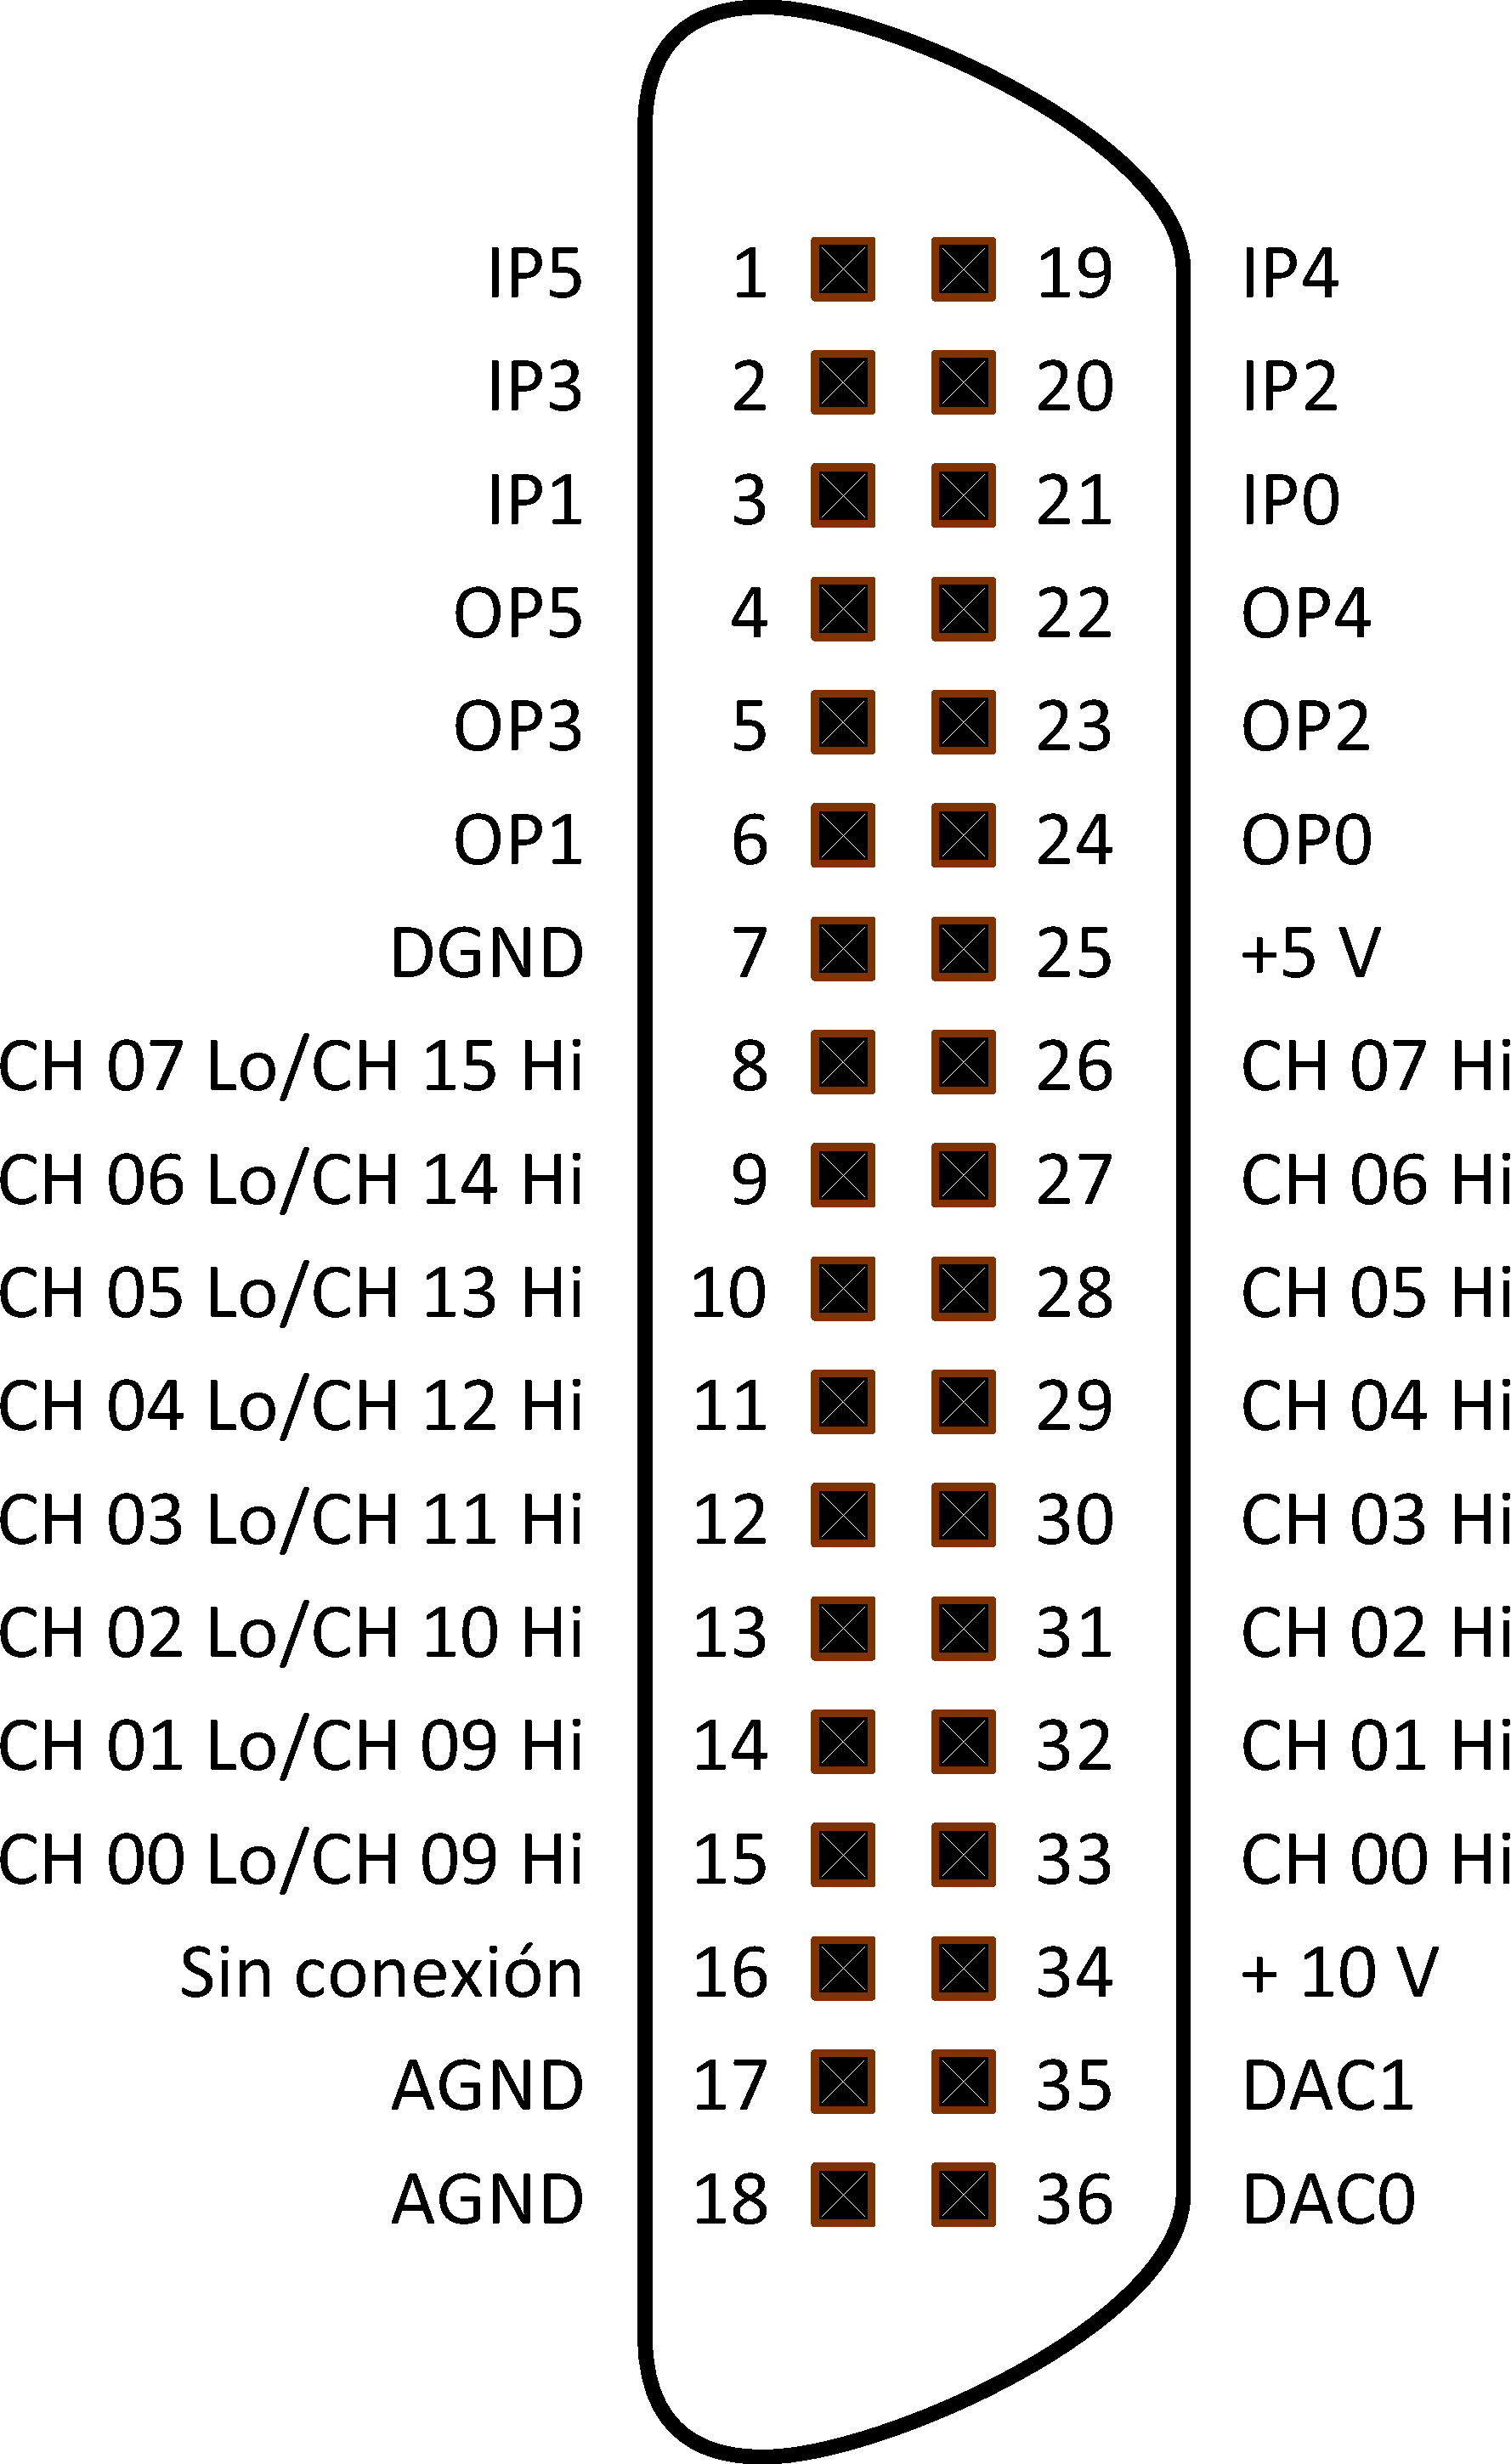
\includegraphics[width=.4\textwidth, keepaspectratio=true]{gis-pfc-ch1-2.pdf}}

\begin{figure}
	\centering
	\subfloat[Conector etiquetado como ``analog'']{%
		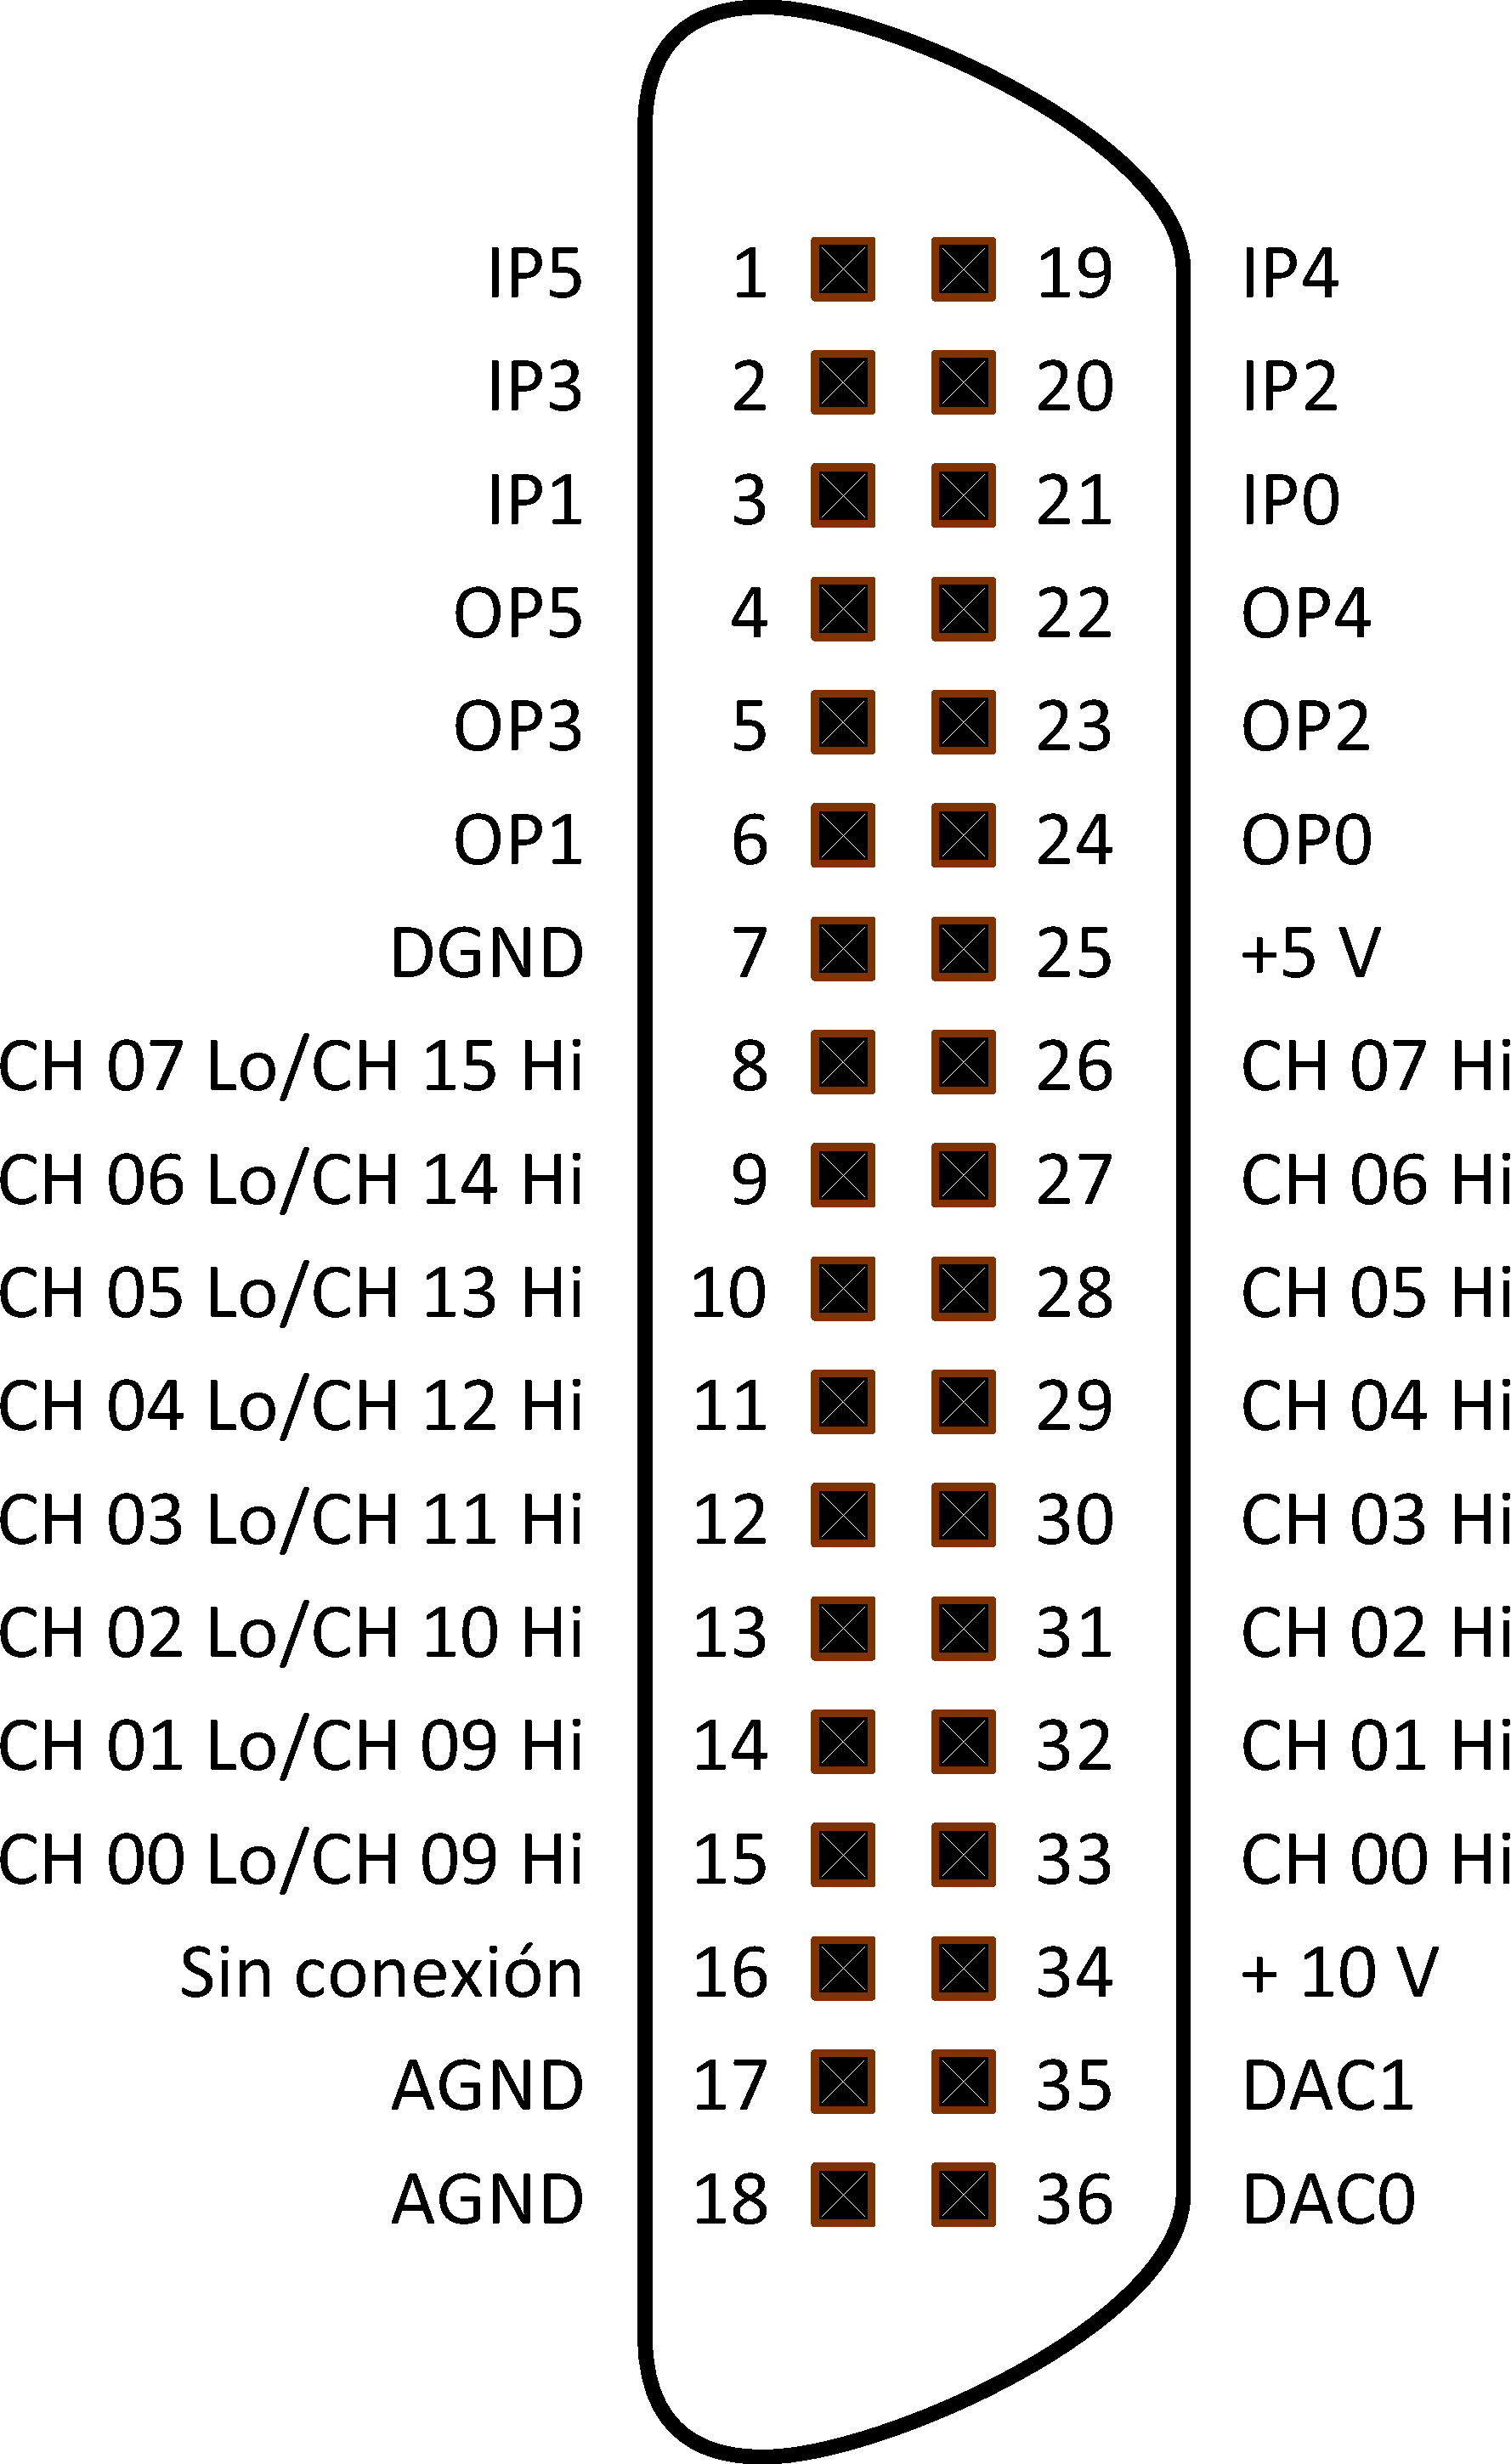
\includegraphics[width=.4\textwidth, keepaspectratio=true]{gis-pfc-ch1-2.pdf}}\qquad
	\subfloat[Conector etiquetado como ``digital'']{%
		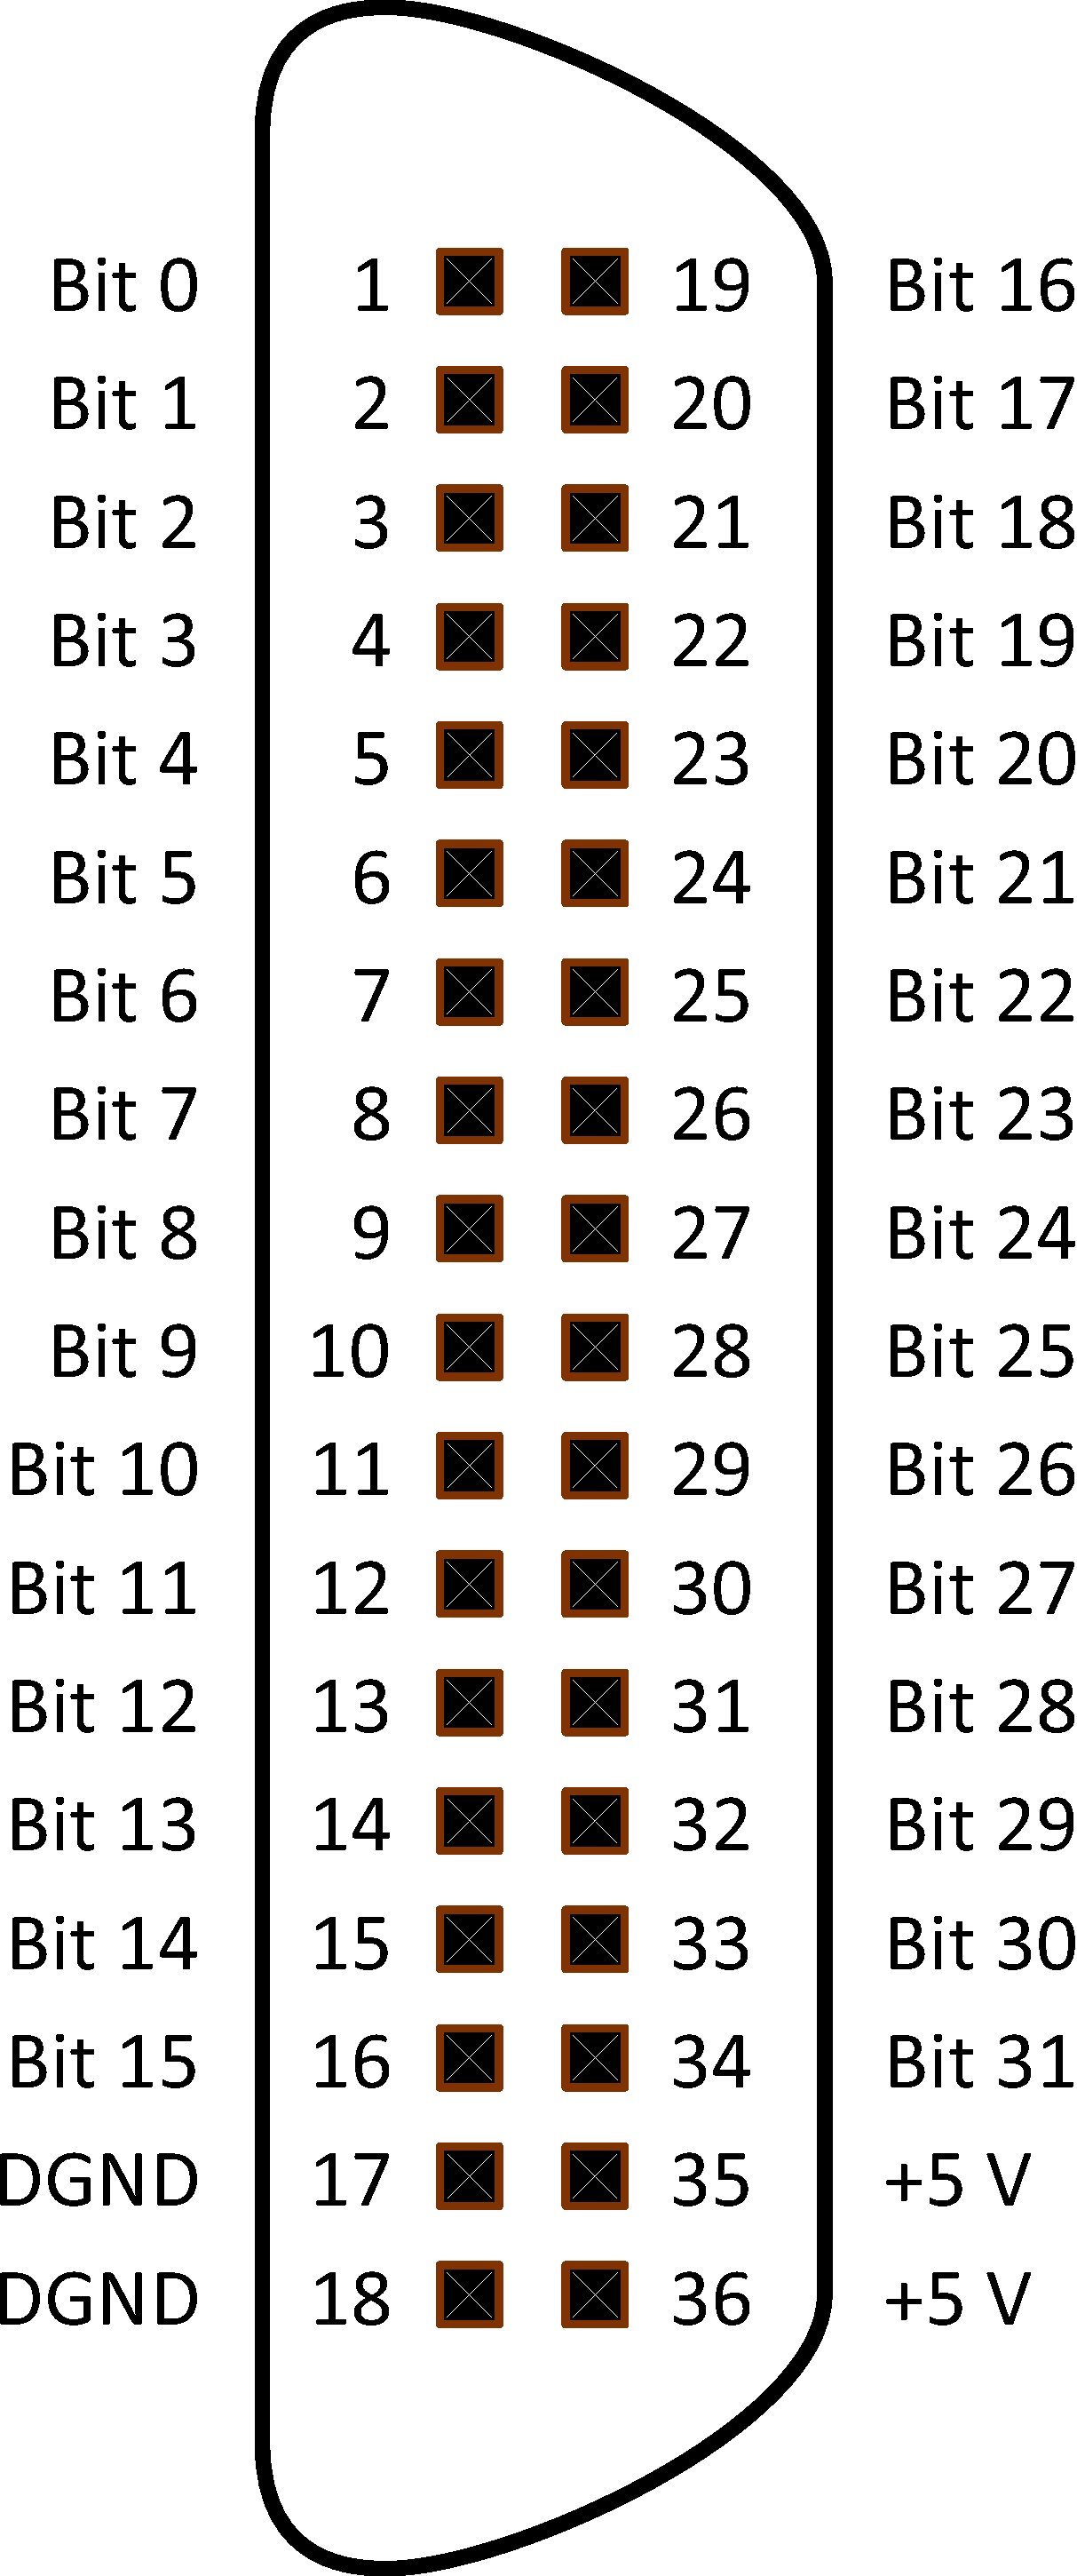
\includegraphics[height=\ht\portbox, keepaspectratio=true]{gis-pfc-ch1-3.pdf}}
 	\caption{Esquema del panel de conexiones trasero de la \kpci{}}
	\label{fig:ports}
\end{figure}


\begin{table}
	\centering
	\begin{tabular}{>{\raggedleft}p{1cm} >{\scshape}c >{\arraybackslash}l}
		\toprule
		\multicolumn{1}{c}{Terminal} & {\upshape Puerto asignado} & \multicolumn{1}{c}{Descripci�n} \\
		\midrule
		1 & ip5 & \multirow{12}{0.6\textwidth}{Bits digitales de entrada multifunci�n. Pueden ser configurados por el usuario para que ejerzan la funci�n de:\miniit{\item Base temporal para el contador/temporizador y/o entrada a \emph{gate} \\\item Reloj externo para conversiones A/D o D/A \\\item Disparador digital externo \\\item Entrada digital en el modo \emph{target-mode}}} \\
		2 & ip3 & \\
		3 & ip1 & \\
		\\\\\\\\\\\\\\\\
		\midrule
		4 & op5 & \multirow{12}{0.6\textwidth}{Bits digitales de salida multifunci�n. Pueden ser configurados por el usuario para que ejerzan la funci�n de:\miniit{\item Salidas del contador/temporizador\\\item Salida del disparador\\\item Salida de control para accesorios\\\item Salida del reloj interno\\\item Salida digital en el modo \emph{target-mode}}} \\
		5 & op3 & \\
		6 & op1 & \\
		\\\\\\\\\\\\\\\\
		\midrule
		7 & dgnd & \multicolumn{1}{c}{Tierra digital} \\
		\midrule
		8 & ch07 lo/ch15 & \multirow{4}{0.6\textwidth}{Entradas anal�gicas, cuya funci�n depende del modo de terminaci�n configurado: puerto asociado a un canal monoterminal o puerto bajo de un canal diferencial} \\
		9 & ch06 lo/ch14 & \\
		10 & ch05 lo/ch13 & \\
		$\vdots$ & $\vdots$ & \\
		15 & ch00 lo/ch08 & \\
		\midrule
		16 & {\upshape Sin conexi�n} & \\
		\midrule
		\multicolumn{1}{l}{17, 18} & agnd & Tierra anal�gica \\
		\bottomrule
	\end{tabular}
	\caption{Relaci�n entre los puertos y terminales que presenta el conector trasero de la \kpci{} etiquetado como \emph{analog}}
	\label{tab:analog}
\end{table}

\begin{table}\ContinuedFloat
	\centering
	\begin{tabular}{>{\raggedleft}p{1cm} >{\scshape}c >{\arraybackslash}l}
		\toprule
		\multicolumn{1}{c}{Terminal} & {\upshape Puerto asignado} & \multicolumn{1}{c}{Descripci�n} \\
		\midrule
		19 & ip4 & \multirow{12}{0.6\textwidth}{Bits digitales de entrada multifunci�n. Pueden ser configurados por el usuario para que ejerzan la funci�n de:\miniit{\item Base temporal para el contador/temporizador y/o entrada a \emph{gate} \\\item Reloj externo para conversiones A/D o D/A \\\item Disparador digital externo \\\item Entrada digital en el modo \emph{target-mode}}} \\
		20 & ip2 & \\
		21 & ip0 & \\
		\\\\\\\\\\\\\\\\
		\midrule
		22 & op4 & \multirow{12}{0.6\textwidth}{Bits digitales de salida multifunci�n. Pueden ser configurados por el usuario para que ejerzan la funci�n de:\miniit{\item Salidas del contador/temporizador\\\item Salida del disparador\\\item Salida de control para accesorios\\\item Salida del reloj interno\\\item Salida digital en el modo \emph{target-mode}}} \\
		22 & op2 & \\
		21 & op0 & \\
		\\\\\\\\\\\\\\\\
		\midrule
		25 & {\upshape +5 V} & \multirow{2}{0.6\textwidth}{Referencia de tensi�n de 5 voltios de corriente continua extra�dos del bus \sig{pci} del ordenador} \\
		& & \\
		\midrule
		26 & ch07 hi & \multirow{3}{0.6\textwidth}{Entradas anal�gicas restantes, en el modo de terminaci�n diferencial representan el puerto alto de un canal diferencial} \\
		27 & ch06 hi & \\
		28 & ch05 hi & \\
		$\vdots$ & $\vdots$ & \\
		33 & ch00 hi & \\
		\midrule
		34 & {\upshape +10 V} & \multirow{6}{.6\textwidth}{Entrada dise�ada para proporcionar al dispositivo una referencia externa de precisi�n de 10 voltios mediante una fuente de alta impedancia de salida (La impedancia de entrada de este puerto es equivalente a una resistencia de 1 k$\Omega$ en serie con la impedancia de entrada de la fuente)} \\
		\\\\\\\\\\
		\bottomrule
	\end{tabular}
	\caption[]{Continuaci�n del \vref{tab:analog}}
\end{table}

\begin{table}\ContinuedFloat
	\centering
	\begin{tabular}{>{\raggedleft}p{1cm} >{\scshape}c >{\arraybackslash}l}
		\toprule
		\multicolumn{1}{c}{Terminal} & {\upshape Puerto asignado} & \multicolumn{1}{c}{Descripci�n} \\
		\midrule
		35 & dac1 & \multirow{2}{.6\textwidth}{Salida n�mero 1 del conversor digital a anal�gico de la \kpci{}} \\
		\\
		\midrule
		36 & dac0 & \multirow{2}{.6\textwidth}{Salida n�mero 0 del conversor digital a anal�gico de la \kpci{}} \\
		\\
		\bottomrule
	\end{tabular}
	\caption[]{Continuaci�n del \vref{tab:analog}}
\end{table}

\begin{table}
	\centering
	\begin{tabular}{>{\raggedleft}p{1cm} >{\scshape}c >{\arraybackslash}l}
		\toprule
		\multicolumn{1}{c}{Terminal} & {\upshape Puerto asignado} & \multicolumn{1}{c}{Descripci�n} \\
		\midrule
		1 & {\upshape Bit 0} & \multirow{6}{0.6\textwidth}{Canal 0 de bits de entrada/salida de prop�sito general (En la \kpci{} los bits digitales se agrupan de en ocho en ocho en canales. Los canales de este tipo puede configurarse para que los bits que lo integran se comporten como todo salidas o todo entradas)} \\
		2 & {\upshape Bit 1} & \\
		3 & {\upshape Bit 2} & \\
		$\vdots$ & $\vdots$ & \\
		8 & {\upshape Bit 7} & \\
		\\
		\midrule
		9 & {\upshape Bit 8} & \multirow{2}{0.6\textwidth}{Canal 1 de bits de entrada/salida de prop�sito general} \\
		10 & {\upshape Bit 9} & \\
		11 & {\upshape Bit 10} & \\
		$\vdots$ & $\vdots$ & \\
		16 & {\upshape Bit 15} & \\
		\midrule
		\multicolumn{1}{l}{17, 18} & dgnd & Tierras digitales \\
		\midrule
		19 & {\upshape Bit 16} & \multirow{2}{0.6\textwidth}{Canal 2 de bits de entrada/salida de prop�sito general} \\
		20 & {\upshape Bit 17} & \\
		21 & {\upshape Bit 18} & \\
		$\vdots$ & $\vdots$ & \\
		26 & {\upshape Bit 23} & \\
		\midrule
		27 & {\upshape Bit 24} & \multirow{2}{0.6\textwidth}{Canal 3 de bits de entrada/salida de prop�sito general} \\
		28 & {\upshape Bit 25} & \\
		29 & {\upshape Bit 26} & \\
		$\vdots$ & $\vdots$ & \\
		34 & {\upshape Bit 31} & \\
		\midrule
		\multicolumn{1}{l}{35, 36} & {\upshape +5 V} & +5 V\sig{dc} desde el bus del ordenador \\
		\bottomrule
	\end{tabular}
	\caption{Relaci�n entre los puertos y terminales que presenta el conector trasero de la \kpci{} etiquetado como \emph{digital}}
	\label{tab:digital}
\end{table}


\subsection{Desarrollo de una nueva interfaz}\label{subsec:conbox}

Por razones pr�cticas, la interfaz original de la \kpci{} basada en dos conectores mini-\sig{d} no se acomoda a las necesidades que se prev� surgir�n durante el desarrollo de las pruebas requeridas para la finalizaci�n de este proyecto de fin de carrera. En consecuencia, con el prop�sito de agilizar en la medida de lo posible la realizaci�n de estos ensayos, se decide ampliar la interfaz existente.\par
Para ello se parte de dos extremos de cable terminados en un conector tipo macho y desprovistos de cubierta, de cada uno de los cuales surgen 36 hilos de cobre recubiertos de pl�stico flexible coloreado. El patr�n de coloreado de las cubiertas individuales es �nico y no se repite en ninguno de los 36 hilos de que se compone cada extremo de cable. A partir de ah�, se identifica cada terminal de cada conector con el hilo de cobre correspondiente, relacionando las etiquetas que el fabricante pone a los terminales con el c�digo de colores de la cubiertas individuales.\par
Una vez recopilada esta informaci�n, se planea la construcci�n de una caja de conexiones. El dise�o de la caja contempla que se equipe �sta con 72 conectores banana hembra soldados a los 72 hilos de cobre y que comunican con los terminales de los conectores mini-\sig{d} en los que termina el otro extremo de los cables. Adem�s se planifica la inclusi�n de cuatro conectores coaxiales con rosca con conexiones redundantes a las que se presupone son las cuatro puertas cuyo uso ser� m�s frecuente, las correspondientes al primer canal anal�gico diferencial y las tierras anal�gicas; para as� facilitar el uso continuado de las mismas. Por �ltimo se decide etiquetar la caja de conexiones con marbetes que reproduzcan la nomenclatura visible en la \vref{fig:ports}.\par
Puede observarse una representaci�n de la caja de conexiones ya terminada en la \vref{fig:conbox}.

\begin{figure}
	\begin{center}
		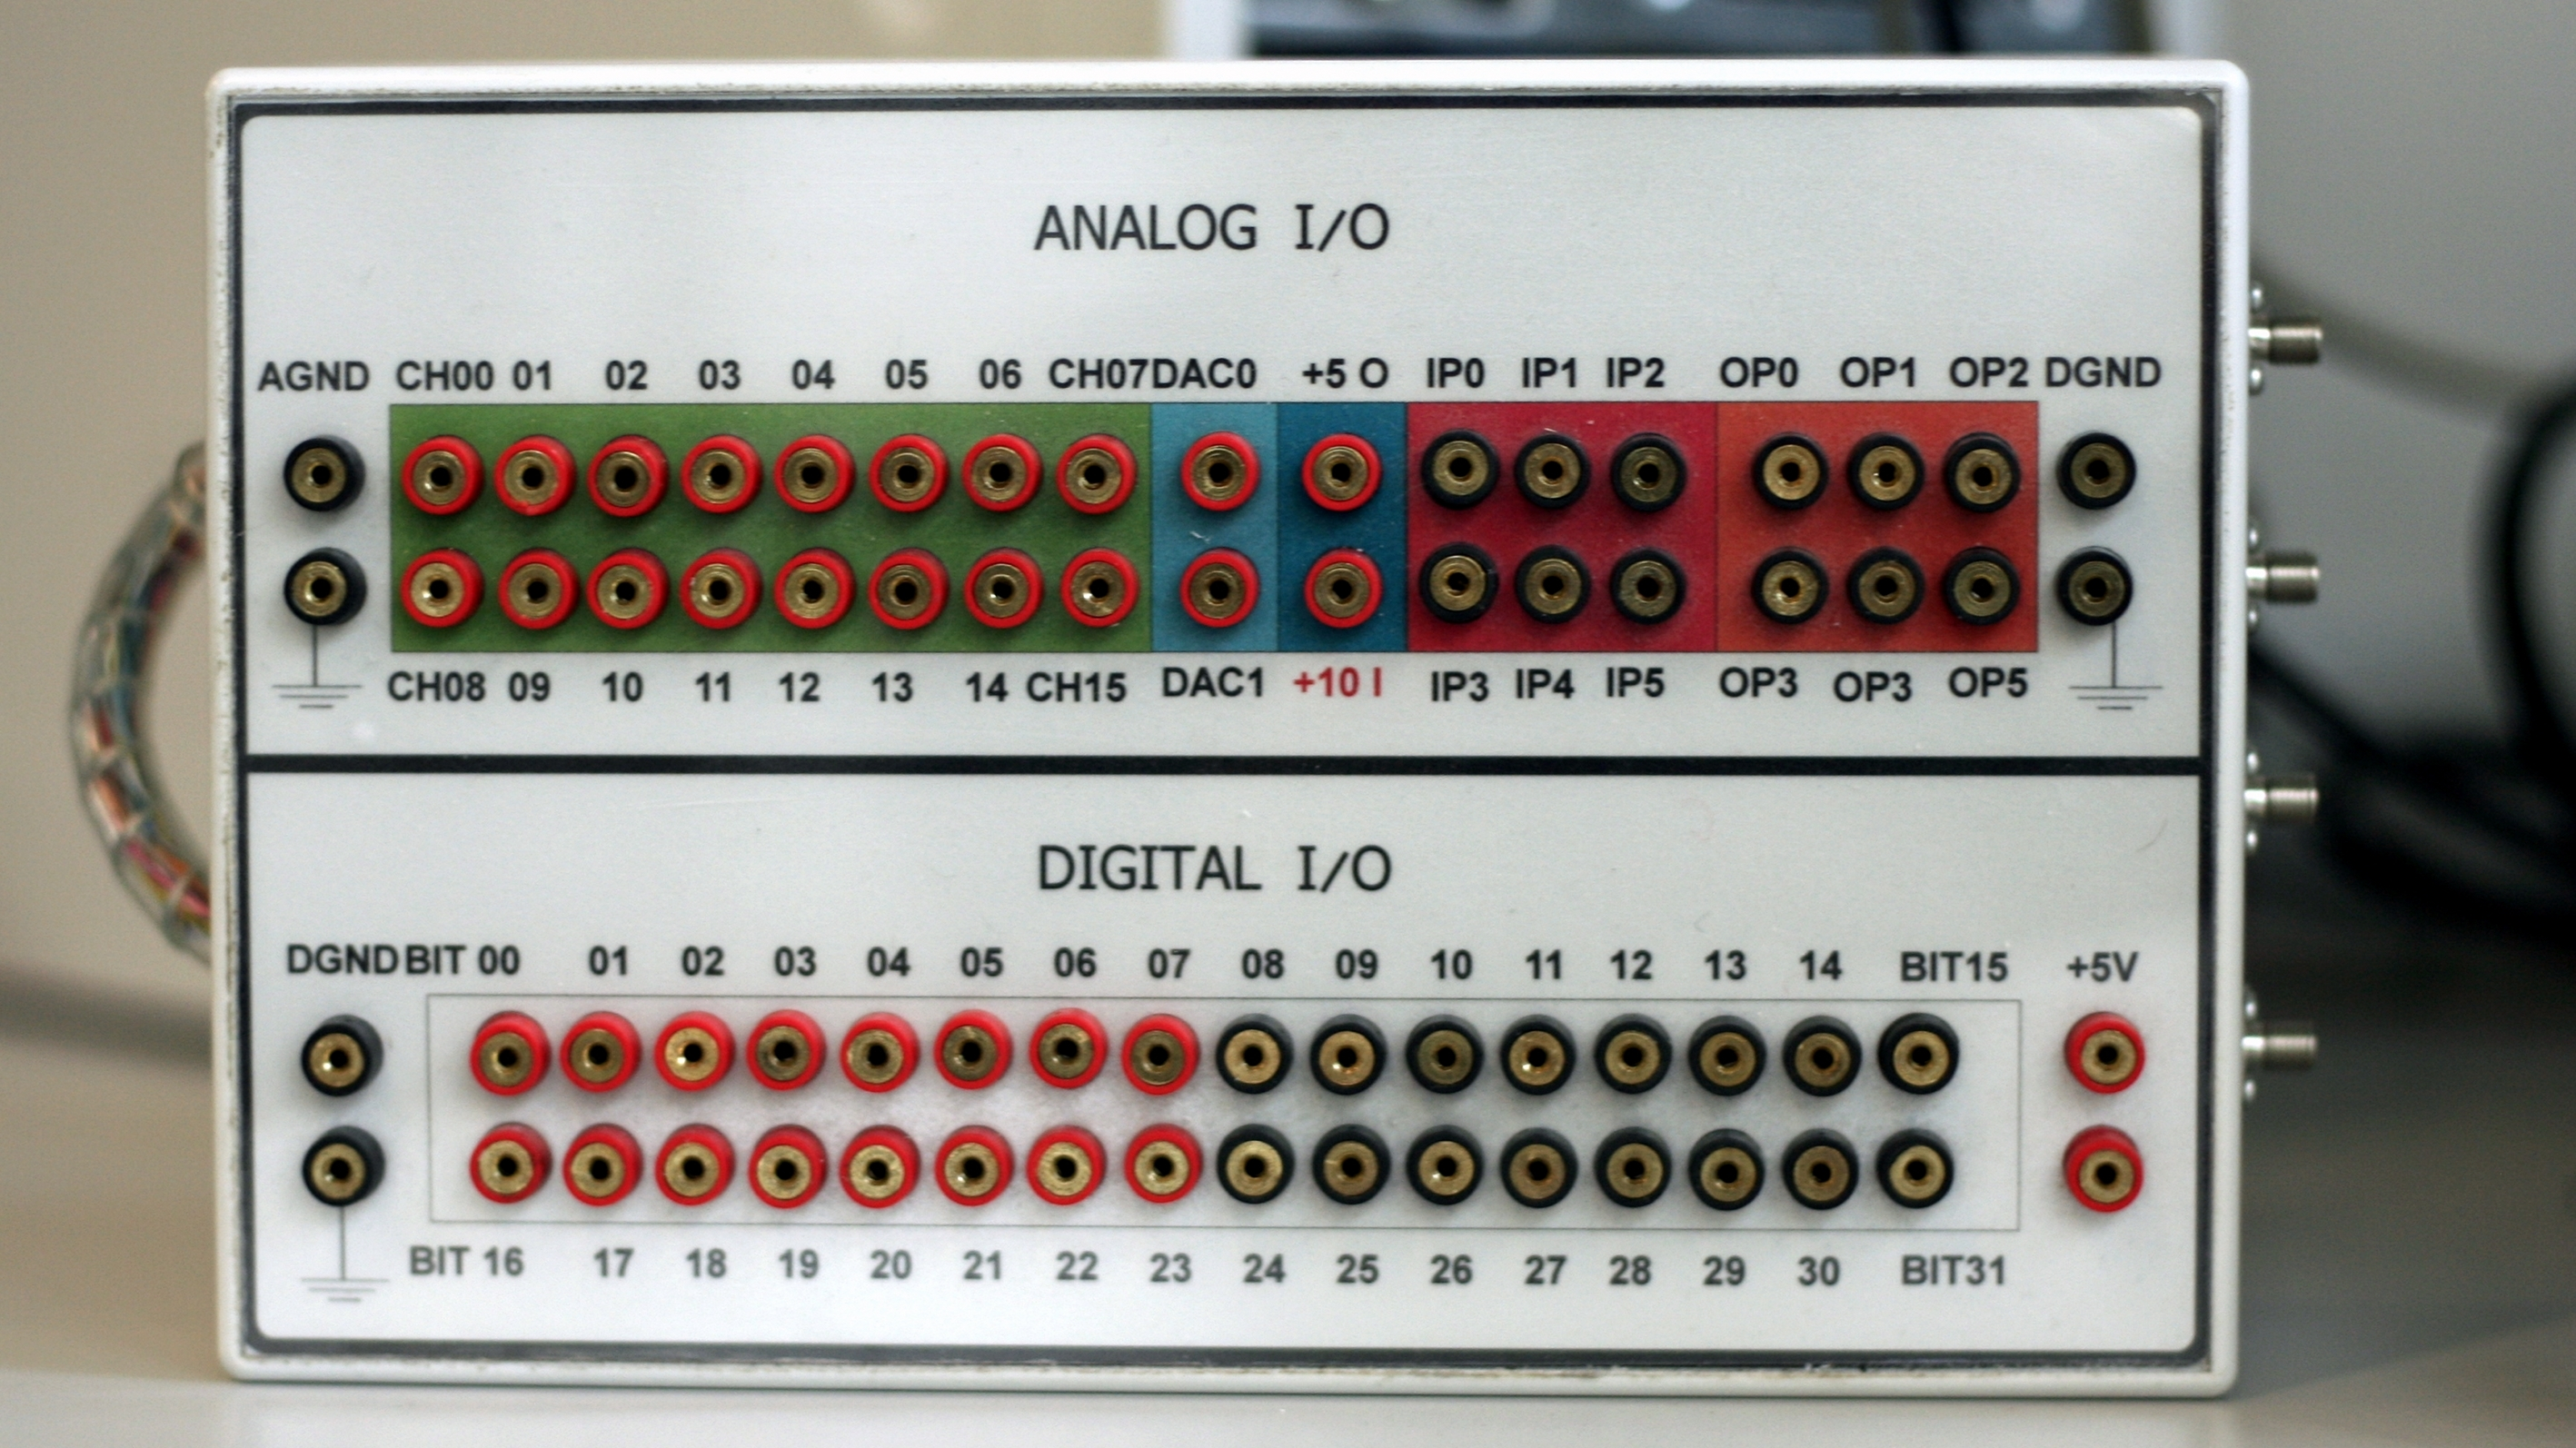
\includegraphics[scale=1, keepaspectratio=true]{gis-pfc-ch1-4.jpg}
	\end{center}
	\caption{Plano de la caja de conexiones ya terminada}
	\label{fig:conbox}
\end{figure}

\chapter{Subsistema de adquisición}

El subsistema de adquisición es el encargado de recibir la señal analógica
procedente del subsistema para la interacción con el medio físico,
muestrearla y proporcionar a las capas superiores una versión digital de la
misma. Es un subsistema exclusivo, y al mismo tiempo distintivo de los
sistemas digitales de medida. En la \cref{fig:subacqui} se muestra una
ventana parcial del sistema de medida digital centrada en las unidades
funcionales que conforman el subsistema de adquisición.

\begin{figure}
	\begin{center}
		\includegraphics{gis-pfc-ch2-01.mps}
	\end{center}
	\caption[Subsistema de adquisición] {Elementos funcionales que
	incluye el subsistema de adquisición.}
	\label{fig:subacqui}
\end{figure}

El subsistema de adquisición del sistema digital de medida propuesto para
el proyecto comprende un único bloque, un bloque de adquisición en el que
se ubica una tarjeta de adquisición. La tarjeta \kpci{} es el fundamento en
el que se basa, no sólo el subsistema de adquisición, si no el sistema
digital de medida al completo. Sus capacidades y muchas de sus limitaciones
las hereda el sistema, y constituyen los principios de diseño del resto de
subsistemas. El subsistema para la interacción con el medio debe proveer al
subsistema de adquisición con una señal que se ajuste a las
especificaciones de la tarjeta, además el circuito acondicionador de
recepción debe adaptar la impedancia de entrada mostrada por el
dispositivo. Por su parte, el subsistema de control y presentación debe ser
capaz de gestionar el funcionamiento de este instrumento y administrar los
valores de señal que proporciona. Además, la \kpci{}, disponer de ella, es
una de las razones principales por las que se ha optado por desarrollar un
sistema de adquisición propio, de propósito, sin tener en cuenta las
principales razones, como es obvio, uno de los objetivos del proyecto,
adquirir conocimientos prácticos en el campo del tratamiento digital de
señales y, por supuesto, contar con un sistema diseñado a medida. Por todas
estas razones, resulta comprensible realizar un estudio previo acerca de
las propiedades y el comportamiento de un instrumento de tan singular
importancia para este proyecto.

Esta memoria dedica un capítulo completo a exponer las características de
la tarjeta \kpci{}. Una breve relación de las características técnicas del
hardware da paso a la descripción funcional, en la que se explica cual es
el comportamiento interno de la tarjeta, como se implementan las distintas
funciones que ofrece. Para terminar el capítulo se reproducen los consejos
que el fabricante proporciona en el manual de usuario con la premisa de que
los usuarios consigan el máximo rendimiento de la tarjeta (punto
\ref{sec:throughput} en la página \pageref{sec:throughput}) y se muestra la
caja de conexiones elaborada expresamente para este proyecto.


\section{Características técnicas del hardware}\label{sec:technical}

La tarjeta \kpci{} puede emplearse para la adquisición y conversión de
señales analógicas en señales digitales, para sintetizar señales analógicas
a partir de señales digitales previamente generadas o almacenadas, o
---gracias a sus 32 puertos digitales de propósito general--- trabajar con
señales digitales.

El subsistema de adquisición dentro del sistema de medida digital requiere
únicamente de la función de adquisición analógica de la tarjeta. Por ello,
de entre todas las características del dispositivo, se ha creído
conveniente resumir a continuación aquellas que tienen relación directa con
dicha función. Para obtener información detallada sobre la relación que
estos atributos guardan con el proceso de adquisición de señales analógicas
en la tarjeta \kpci{}, véase la \vref{sec:funcdesc}.

\begin{itemize}
	\item El módulo de adquisición analógica dispone de 16 puertos
		físicos.
	\item La impedancia de entrada equivalente de cada puerto es
		aproximadamente igual a una capacidad de 200 pF en serie
		con una resistencia de valor inferior, pero aproximadamente
		igual, a 1 k$\Omega$.
	\item En condiciones óptimas, es posible conseguir un rendimiento
		máximo de 100 \kms{} (cien mil operaciones de conversión
		por segundo). Este valor está sujeto a un error relativo
		del $0.02\%$.
	\item La resolución del conversor analógico digital es de 16 bits
		por muestra. El rango de amplitudes en el que opera depende
		de como esté configurado el modo de adquisición. Puede ir
		de 0 V a 10 V si el modo de adquisición es unipolar, o de
		-10 V a 10 V si es bipolar.
	\item La cola de muestreo tiene capacidad para hasta 256 canales
		distintos. Cada uno de los cuales puede configurarse
		independientemente en términos de ganancia, frecuencia de
		muestreo, modo de adquisición o modo de terminación.
	\item La ganancia, responsable en parte de la resolución con la que
		se cuantifica las muestras, puede tomar cada ciclo de reloj
		uno de entre 16 valores posibles (véase el
		\vref{tab:acqmodes}).
\end{itemize}


\section{Descripción funcional}\label{sec:funcdesc}

Es necesario programar el comportamiento de la tarjeta de adquisición antes
de ponerla en funcionamiento. Desde la cola de muestreo se controlan los
principales aspectos del proceso de adquisición, como por ejemplo, en que
instantes se encuentra activo.

La cola de muestreo, como su propio nombre indica, es una estructura de
datos ordenada. Se encuentra almacenada en una memoria \sig{ram} de 256
entradas que forma parte del hardware de la tarjeta. En el \cref{tab:queue}
puede verse una representación de un ejemplo de la cola de muestreo.

\begin{table}
	\centering
	\begin{threeparttable}
	\begin{tabular}{lccccccccc}
		\toprule
		Posición en la cola & 1 & 2 & 3 & 4 %
		& \multicolumn{2}{c}{$\cdots$} & 254 & 255 & 256 \\
		\midrule
		Número de canal & 15 & 15 & 02 & 02 %
		& \multicolumn{2}{c}{$\cdots$} & 17 & 13 & 01 \\
		Número de puerto & 07 & 07 & 11 & 11 %
		& \multicolumn{2}{c}{$\cdots$} & 07 & 09 & 01 \\
		Ganancia & 1 & 1 & 40 & 40 %
		& \multicolumn{2}{c}{$\cdots$} & 200 & 8 & 80 \\
		Modo de adquisición\tnote{a} & $\pm$ & $\pm$ & $+$ & $+$ %
		& \multicolumn{2}{c}{$\cdots$} & $\pm$ & $+$ & $\pm$ \\
		Modo de terminación\tnote{b} & \sig{d} & \sig{d} %
		& \sig{m} & \sig{m} & \multicolumn{2}{c}{$\cdots$} %
		& \sig{d} & \sig{m} & \sig{m}\\
		\bottomrule
	\end{tabular}
	\begin{TableNotes}
		\tnotetext{a}{Configuración bipolar ($\pm$), configuración
		unipolar ($+$).}
		\tnotetext{b}{Canal diferencial (\sig{d}), canal
		monoterminal (\sig{m}).}
	\end{TableNotes}
	\end{threeparttable}
	\caption[Ejemplo de cola de muestreo]{Ejemplo de cola de muestreo.}
	\label{tab:queue}
\end{table}

Cada entrada en la memoria \sig{ram} se identifica con una posición en la
cola. Las posiciones en la cola pueden encontrarse vacías o estar ocupadas
por un canal. Varias posiciones en la cola, consecutivas o no, pueden estar
ocupadas por un mismo canal. Por tanto, la cola puede estar ocupada, como
máximo, por 256 canales independientes.

Las posiciones ocupadas contienen información correspondiente al canal y a
los atributos asociados a este. Un canal es una entidad lógica que
relaciona un puerto físico con un búffer de información y una serie de
atributos. Durante el proceso de adquisición un puntero recorre las
distintas posiciones de la cola, una a una y en orden. El canal activo,
aquel que ocupa la posición a la que apunta el puntero en cada ciclo de
reloj, determina tres cosas:

\begin{itemize}
	\item De qué puerto debe proceder la señal analógica\footnote{Por
		convenio se ha elegido hablar de una sola señal que entra
		al amplificador. Si se ha hecho esta elección, es porque si
		bien al amplificador pueden entrar una o dos señales
		simultáneamente, esto no supone otra diferencia para el
		proceso que la expuesta en el \vref{subsubsec:termmodes}.
		Es por ello, y para mantener la claridad, que se ha omitido
		esta posibilidad.} que llega al amplificador de
		instrumentación interno de la tarjeta.
	\item En qué búffer debe almacenarse el valor resultante de
		muestrear y cuantificar esta señal.
	\item Por último, los atributos asociados al canal: ganancia, modo
		de adquisición y modo de terminación; indican,
		respectivamente: cual debe ser la ganancia del amplificador
		de instrumentación, cual debe ser el rango de trabajo del
		conversor analógico digital, y que se debe conectar a los
		terminales de entrada del amplificador de instrumentación.
		Se da más información al respecto en apartados
		subsiguientes.% la polaridad de las muestras y el número de
		% terminales de entrada, uno o dos dependiendo de si la
		% adquisición es diferencial o no, durante el ciclo actual.
\end{itemize}

Para concluir el apartado cabe remarcar lo siguiente. Es posible inferir
dos cosas de esta mecánica de funcionamiento basada en la cola. Una de
ellas es que el proceso de adquisición afecta a una sola señal cada vez. Y
la segunda, que la frecuencia de muestreo ligada a un canal depende de dos
factores, de la velocidad de la señal de reloj, y de la cantidad de veces
que un canal aparece repetido en la cola.


\subsection{Métodos de entrada}

La \kpci{} permite dos modos de adquisición y dos modos de terminación.
Aprender a diferenciar cuando es oportuno seleccionar entre cada uno de
ellos beneficiará la calidad de la señal digital resultante.


\subsubsection{Modos de adquisición}

Una señal es bipolar cuando toma valores positivos y negativos. Por el
contrario, se distingue a las señales unipolares porque todos sus valores
mantienen la misma polaridad, ya sea ésta positiva o negativa. Para cada
canal, debe configurarse el modo de adquisición como bipolar o
unipolar\footnote{La tarjeta \kpci{} sólo admite señales unipolares de
polaridad positiva.} atendiendo a la señal de interés.

Si se sabe a ciencia cierta que la señal de entrada es unipolar debe
emplearse el modo de adquisición unipolar. De ese modo, se duplica la
resolución del conversor analógico digital.

\begin{sidewaystable}
	\centering
	\begin{tabular}{>{\raggedleft}p{1.2cm}d{5.2}d{3.1}+d{3.1}}
		\toprule
		& \multicolumn{2}{c}{Bipolar} %
		& \multicolumn{2}{c}{Unipolar} \\
		\cmidrule(r){2-3}\cmidrule(l){4-5}
		\multicolumn{1}{c}{Ganancia}
		& \multicolumn{1}{c}{Rango ($\pm\text{V}$)} %
		& \multicolumn{1}{c}{Precisión ($\mu\text{V}$)} %
		& \multicolumn{1}{c}{Rango (V)} %
		& \multicolumn{1}{c}{Precisión ($\mu\text{V}$)} \\
		\midrule
		1 & 10,0 & 305 & 0/$10,0$ & 153 \\
		2 & 5,0 & 153 & 0/$5,0$ & 76 \\
		4 & 2,5 & 76 & 0/$2,5$ & 38 \\
		8 & 1,25 & 38 & 0/$1,25$ & 19 \\
		10 & 1,0 & 31 & 0/$1,0$ & 15 \\
		\\
		& \multicolumn{2}{c}{Bipolar} %
		& \multicolumn{2}{c}{Unipolar} \\
		\cmidrule(r){2-3}\cmidrule(l){4-5}
		\multicolumn{1}{c}{Ganancia}
		& \multicolumn{1}{c}{Rango ($\pm\text{mV}$)} %
		& \multicolumn{1}{c}{Precisión ($\mu\text{V}$)} %
		& \multicolumn{1}{c}{Rango (mV)} %
		& \multicolumn{1}{c}{Precisión ($\mu\text{V}$)} \\
		\midrule
		20 & 500 & 15 & 0/500 & 7,6 \\
		40 & 250 & 7,6 & 0/250 & 3,8 \\
		80 & 125 & 3,8 & 0/125 & 1,9 \\
		100 & 100 & 3,1 & 0/100 & 1,5 \\
		200 & 50 & 1,5 & 0/50 & 0,8 \\
		400 & 25 & 0,8 & 0/25 & 0,4 \\
		800 & 12,5 & 0,4 & 0/$12,5$ & 0,2 \\
		\bottomrule
	\end{tabular}
	\caption[Relación entre ganancia, rango de trabajo y resolución
	según el modo de adquisición]{Relación entre ganancia, rango de
	trabajo y resolución según el modo de adquisición.}
	\label{tab:acqmodes}
\end{sidewaystable}


\subsubsection{Modos de terminación}\label{subsubsec:termmodes}

Internamente, la tarjeta \kpci{} emplea un amplificador de instrumentación
diferencial. En principio este hecho implicaría que a cada canal se
asociasen dos puertos físicos, uno por cada uno de los dos terminales de
entrada del amplificador. No obstante, es posible configurar la tarjeta
para que uno de los terminales del amplificador se conecte a masa. En ese
caso, el terminal restante se conecta a un puerto físico. La
\vref{fig:termmodes} muestra un ejemplo de esta configuración.

\begin{figure}
	\begin{center}
		\includegraphics{gis-pfc-ch2-02.mps}
	\end{center}
	\caption[Ejemplo de configuración de terminación]{Figura que
	muestra el modo de terminación sencillo. La entrada superior del
	amplificador de instrumentación se conecta al puerto 9 y la entrada
	inferior se conecta a masa.}
	\label{fig:termmodes}
\end{figure}

Para habilitar semejante configuración, cabría pensar que es suficiente con
modificar el atributo que controla el modo de terminación del canal
correspondiente. Al contrario de lo que pudiera parecer, el modo de
terminación es una propiedad que no es atribuible al canal, si no que se
atribuye a un par de puertos\footnote{Aunque según las especificaciones del
fabricante es posible configurar cada par de puertos para que opere según
un modo de terminación independiente del resto, el entorno de desarrollo
utilizado durante el proyecto sólo admite un modo de terminación para el
conjunto total de puertos (v. el \vref{chap:control}).}. En concreto, el
modo de terminación afecta a los pares de puertos compuestos por un primero
de entre los puertos 0 y 7, y un segundo cuyo número de puerto es igual al
del primero más 8. De ahí que todos los canales relacionados con el mismo
par de puertos deban estar configurados con el mismo modo de terminación,
una configuración distinta no está permitida.

Los dos modos de terminación posibles se conocen como: diferencial, si es
que la señal que entra en cada terminal del amplificador procede de cada
uno de los puertos del par; sencillo, en caso de que uno de los terminales
de entrada del amplificador se conecte a la referencia de tensión. En este
documento se llama canal diferencial a los canales cuyo modo de terminación
sea diferencial, y canal con un sólo terminal o monoterminal a aquellos
para los que el modo de terminación es sencillo.

Las ventajas que presenta el uso de uno u otro tipo de canales son
comprensibles. Emplear canales con un sólo terminal permite aplicar el
proceso de adquisición sobre un mayor número de señales simultáneamente.
Por el contrario, utilizar canales diferenciales redunda en una mayor
inmunidad frente al ruido. Además, los amplificadores diferenciales
eliminan de forma inherente la componente en continua.


\section{Rendimiento}\label{sec:throughput}

En el ámbito de este documento se entiende como rendimiento de la tarjeta
de adquisición la cantidad máxima de operaciones de conversión que el
dispositivo puede realizar por unidad de tiempo. Para que una de estas
operaciones contribuya a la medida de rendimiento debe superar un requisito
de precisión.

El rendimiento óptimo de la tarjeta \kpci{} especificado por el fabricante
es de cien mil operaciones por segundo (100 \kms{}). No obstante se
advierte, para obtener este nivel de rendimiento es necesario alimentar la
tarjeta con una fuente de tensión ideal. Además, es importante que exista
adaptación de impedancias entre el circuito de alimentación y el puerto por
el que se quiere introducir la señal. Aún en estas condiciones el valor
proporcionado por la casa Keithley está sujeto a un error relativo máximo
del $0.02\%$, el cual supone un error absoluto máximo de dos mil
operaciones por segundo (2 \kms{}).

En los \sig{endus}, existe una relación directa entre la resolución, la
capacidad de distinguir entre dos defectos próximos, y la frecuencia de
oscilación de la señal ultrasónica. Cuanto mayor sea la frecuencia de las
ondas acústicas mejor la resolución. Los transductores utilizados en el
ensayo se comportan como filtros además de como transductores, ya que por
un lado sólo dejan pasar determinadas componentes de frecuencia y por otro
transforman variaciones de la tensión eléctrica en variaciones de presión o
viceversa. Imponen un límite físico a la frecuencia de oscilación de la
señal ultrasónica y, por tanto, en la resolución. Para trabajar con señales
acústicas de alta frecuencia son necesarios transductores adecuados que
presenten un gran ancho de banda y sean capaces de transmitir las altas
frecuencias. El receptor transforma el pulso acústico en un pulso eléctrico
filtrado, después esta señal se acondiciona y deja el subsistema para la
interacción con el medio físico para pasar al subsistema de adquisición. En
el subsistema de adquisición el pulso eléctrico se muestrea y es ahí donde
entra en juego el rendimiento de la \kpci{}. El teorema de Nyquist estipula
una frecuencia de muestreo mínima para la cual no se produce una pérdida de
información al muestrear una señal periódica y limitada en banda. La
frecuencia de Nyquist es igual al doble de la frecuencia de oscilación
máxima de la señal que se preve muestrear. Si una señal se muestrea a una
tasa inferior se da una pérdida de información y no es posible recuperar la
señal original. En otras palabras, para una frecuencia de muestreo fija,
sólo las señales que oscilan a frecuencias por debajo de la mitad de la
frecuencia de muestreo son correctamente muestreadas. De lo que se deduce
que, cuanto mayor sea el rendimiento del bloque de adquisición, mayor la
frecuencia de las señales que pueden muestrearse sin pérdidas, lo que
implica que no existe impedimento para emplear un receptor de mayor
frecuencia, y asimismo es posible alcanzar una mejor resolución en los
ensayos. Si se emplean transductores de alta frecuencia, y el receptor
genera una señal de frecuencia superior a la mitad del rendimiento del
dispositivo de adquisición, el beneficio de trabajar con señales de alta
frecuencia no es real. Este es el principal motivo que fomenta el interés
por extraer el mayor rendimiento de la tarjeta \kpci{}. Para lograrlo es
necesario conocer por un lado que factores limitan el rendimiento de la
tarjeta y, por otro, como debe configurarse el dispositivo para que la
influencia de esos factores sea mínima.


\subsection[El amplificador de instrumentación] {Amplificador de
instrumentación y pérdida del rendimiento}

El amplificador de instrumentación interno de la \kpci{} es de ganancia
variable. Es posible configurar una ganancia distinta para cada canal. El
propósito del amplificador es permitir al usuario modificar la amplitud de
la señal que entra al conversor. La intención que se persigue es conseguir
que la conversión se enfoque en los detalles de la señal que sean de mayor
interés y se pierda la mínima información posible. Todo ello aún trabajando
simultáneamente con múltiples señales cuyo rango de amplitudes es con
frecuencia muy diferente.

La desventaja que presenta esta configuración ---multiplexor, amplificador
de instrumentación, conversor--- es una pérdida de rendimiento que se
produce en situaciones determinadas a causa de la intervención del
amplificador en la operación de adquisición.

Cada ciclo de reloj cambia el canal activo y debe cambiar, si es oportuno,
la señal que accede al amplificador. Este proceso no es inmediato. Tras
conmutar el multiplexor que precede al amplificador, se da paso al puerto
conveniente. No obstante, la señal que recibe el amplificador presenta,
hasta transcurrido un determinado periodo de tiempo, una componente
residual de la señal que se amplificó en el anterior ciclo de reloj.
Transcurrido dicho periodo de tiempo la señal que entra al amplificador se
ve libre de esa componente residual y se corresponde únicamente con la
señal que entrega el multiplexor, se dice que se ha fijado la señal.

Y es así como el amplificador es causa de pérdida de rendimiento, por medio
de las componentes residuales. Si la conversión se realiza antes de fijar
la señal, el conversor toma un valor de la señal corrompido por la
componente residual de la señal precedente. Por tanto, la muestra
resultante queda igualmente corrompida incluso hasta el punto de perder su
validez. Las operaciones de conversión que tengan como resultado muestras
inválidas sólo contribuyen a falsear la medida de rendimiento, haciendo que
parezca mayor de lo que en realidad es.

El fabricante da a entender que existe una solución de diseño que resuelve
en parte el problema planteado por las componentes residuales. Esta
solución consiste en alargar de forma deliberada la duración del ciclo de
reloj, de esa forma se proporciona tiempo suficiente para fijar la señal.
Sin embargo, esta solución presenta dos inconvenientes: no solventa el
problema en la totalidad de los casos y es, asimismo, una forma de perder
rendimiento. Lo cual conduce inevitablemente a una solución de compromiso,
alargar el ciclo de reloj lo suficiente para que en la mayoría de los casos
el efecto de las componentes residuales sobre la precisión de la conversión
no invalide las muestras resultantes y se produzca, por tanto, una caída
del rendimiento, sin que la duración del nuevo ciclo contribuya por sí
misma a una pérdida notable de éste.


\subsection{Factores que limitan el rendimiento}

Como se ha visto, la inclusión del amplificador en el diseño de la tarjeta
es causa directa o indirecta de una pérdida de rendimiento. La magnitud de
esa caída en el rendimiento depende de la configuración de la cola de
muestreo y de la amplitud de la señal una vez llega ésta al dispositivo de
adquisición.

\subsubsection{Pequeña señal}

Las señales cuya tensión absoluta se encuentra por debajo de los 100 mV al
llegar a la \kpci{} sufren en mayor medida las consecuencias del empleo de
un amplificador en la operación de conversión. En primer lugar la señal
tarda más en fijarse de modo que el rendimiento se reduce a la mitad en las
mejores condiciones, de 100 \kms{} pasa a 50 \kms{}. Esto es debido a que,
al ser la amplitud de la señal y la del ruido comparables, especialmente
después de que éste se vea reforzado por el efecto de las componentes
residuales, se genera una mayor incertidumbre.

Por otro lado las señales que requieren que el amplificador opere con alta
ganancia son las más perjudicadas por los problemas que causa el
amplificador en configuraciones multiganancia, tal y como se explica a
continuación.


\subsubsection{Configuraciones multiganancia}

Por lo general, el rendimiento se ve afectado de forma más pronunciada por
el efecto de las componentes residuales en configuraciones multiganancia en
las que se encadenan secuencias de canales con ganancia diferente. Una
configuración multiganancia de la cola de muestreo implica que en
diferentes ciclos de reloj el amplificador actúa con ganancias distintas.
Eso con frecuencia significa que el rango en el que se encuentra
comprendida la amplitud de las señales que están entrando al dispositivo de
adquisición es diferente de una señal a otra. Cuando así ocurre puede
sucederse en ocasiones que en ciclos de reloj consecutivos entren al
amplificador dos señales de amplitud diferente, siendo la amplitud de la
señal que ocupa el primer ciclo mucho mayor que la de la otra señal en el
tiempo en el que ambas permanecen a la entrada del dispositivo. Por otro
lado, parece lógico considerar que la componente residual asociada a una
señal cuya amplitud sea predominantemente mayor que la de otra señal es de
mayor amplitud inicial y mayor duración temporal que la asociada a la
segunda señal. Por tanto si ocurre como se ha dicho y se tiene en cuenta la
base probable que se ha propuesto, cuando la segunda de las señales se
convierte en la señal activa la amplitud de la componente residual asociada
a la primera de ellas puede ser suficiente, incluso, para enmascararla.

No sólo eso, la amplitud de la señal que llega más tarde al amplificador
puede ser, en términos absolutos, la mayor parte del tiempo, menor que la
de la otra señal, al ser así lo más probable es que se amplifique empleando
un mayor factor de ganancia. De ser así, la amplitud de la componente
residual a la que se enfrenta esta señal puede provocar en el peor de los
casos que el conversor sature y la pérdida de precisión sea mucho mayor.
Sea cual sea el caso, es posible observar entonces, que en configuraciones
multiganancia las muestras resultantes se obtienen de una conversión menos
precisa, en especial si se trabaja con señales de pequeña amplitud ---tal y
como se especificó en el punto anterior--- o si las ganancias configuradas
en la cola de muestreo difieren mucho unas de otras. Aplicando la relación
entre la validez de las muestras y el rendimiento de la que se habló
anteriormente, la consecuencia de emplear configuraciones multiganancia es
una mayor pérdida de rendimiento.


\subsubsection{Configuraciones monoganancia}

En configuraciones monoganancia el uso del amplificador supone una causa
indirecta de la caída de rendimiento. El diseño del dispositivo de
adquisición está pensado primordialmente para su uso en configuraciones
multiganancia, de lo contrario la inclusión de un amplificador de ganancia
variable en el esquemático de la tarjeta sería incomprensible. Por la misma
razón, Keithley adopta una solución de diseño como la expuesta en el
anterior apartado, para tratar de obtener un rendimiento óptimo en
configuraciones multiganancia. Sin embargo, el efecto de las componentes
residuales en configuraciones monoganancia es mínimo y la consecuente
pérdida de rendimiento también lo es. Por tanto, una solución que consiste
en alargar el ciclo de reloj resulta, en configuraciones monoganancia,
innecesaria y perjudicial para el rendimiento.


\subsection{Configuración óptima de la cola de muestreo}

Las acciones que el fabricante adopta para tratar de que el usuario obtenga
el mayor rendimiento posible del dispositivo no se limitan a aplicar una
solución de compromiso en el diseño de la duración del ciclo de reloj. En
el manual de usuario se hacen una serie de recomendaciones de uso
orientadas a conseguir este fin.

Se proponen varias soluciones, de las cuales la solución trivial pasa por
preamplificar todas las señales que vayan a ser objeto del proceso de
adquisición efectuado por la tarjeta consiguiendo que su amplitud varíe en
un mismo rango. Si se hace así, es suficiente con emplear una configuración
monoganancia para minimizar los efectos de las componentes residuales en el
rendimiento. Además al preamplificar las señales, éstas presentan una mejor
relación señal a ruido, es decir, son menos vulnerables al ruido. Aunque
buena, esta solución no deja de ser trivial puesto que el amplificador de
instrumentación de la tarjeta pierde toda funcionalidad y pasa a ser un
estorbo en el proceso de adquisición.

La solución de carácter práctico propuesta por Keithley radica configurar
la cola de muestreo de forma minuciosa, persiguiendo optimizar el
rendimiento. Como se ha visto, en determinadas ocasiones una configuración
inapropiada de la cola de muestreo puede inducir que la pérdida de
productividad que provoca la inclusión del amplificador en el circuito de
adquisición sea todavía mayor. Para evitar que esto ocurra y sacar el
máximo partido del dispositivo se dan en el manual dos condiciones que de
cumplirse garantizan que la cola se encuentre configurada de forma óptima
en términos de rendimiento.


\subsubsection{Agrupaciones de canales}

La primera consiste en agrupar canales con distinta ganancia en posiciones
consecutivas de la cola, aún si al hacerlo se pierde el orden de muestreo
definido en una primera instancia por el usuario. Si como se presupuso en
el apartado anterior, comúnmente dos señales que requieren ser amplificadas
con el mismo factor de ganancia varían en el mismo rango de amplitudes, en
estas secuencias monoganancia las consecuencias de las componentes
residuales en la precisión de la conversión son mínimas.


\subsubsection{Posciones consecutivas}

A pesar de emplear una configuración como la anterior, la aparición de
saltos de ganancia en la cola de muestreo es todavía probable. Por ejemplo,
en la transición entre dos secuencias monoganancia como las descritas
arriba. El salto es aún más problemático si la transición se realiza para
dar paso a una secuencia de ganancia mayor. El primer canal de esta
secuencia sufre en mayor proporción los efectos de las componentes
residuales y el rendimiento asociado al canal se ve reducido
dramáticamente. Para minimizar el impacto que en determinados canales como
éste tienen los problemas causados por el amplificador, es posible
modificar la configuración de la cola para que dichos canales ocupen varias
posiciones consecutivas. Esta segunda condición persigue dar más tiempo
para que se fije la señal cuando los mencionados canales están activos.
Para ello se necesitan posiciones vacías en la cola, posiciones que es
posible obtener desalojando canales previamente configurados.


\section{Comunicación con el periférico}

Para la interacción con dispositivos externos, la \kpci{} dispone de dos
conectores formato mini-\sig{d} de 36 terminales que cumplen con el
estándar \sig{ieee} 1284 de protocolos de comunicación en paralelo. Si se
observa la tarjeta como el rectángulo que forma desde un punto de vista
geométrico y observándola de frente, los conectores quedan ubicados en un
lado de la tarjeta contiguo a aquel en el que se sitúa la conexión
\sig{pci}. Todo ello de forma que tras el montaje del periférico en la
placa base los conectores quedan expuestos en la parte posterior de la
carcasa en la que providencialmente debe encontrarse instalada dicha placa,
tal y como es habitual en este tipo de dispositivos.

En las \cref{fig:portanalog,fig:portdigital} se etiqueta cada terminal
según su ubicación relativa con respecto al conector y al resto de
terminales en el mismo, para cada conector, mostrando la distribución
definida por el fabricante. Los \cref{tab:analog,tab:digital} describen el
propósito de cada terminal y se especifica que tipo de señal debe circular
por los mismos.

\begin{figure}
	\begin{center}
		\subfloat[Conector etiquetado como \guillemotleft
		analog\guillemotright][Conector etiquetado como
		\guillemotleft analog\guillemotright.]{ %
			\label{fig:portanalog} %
			\includegraphics{gis-pfc-ch2-03.mps}}
			\vspace*{.1\textheight}
		\subfloat[Conector etiquetado como \guillemotleft
		digital\guillemotright][Conector etiquetado como
		\guillemotleft digital\guillemotright.]{ %
			\label{fig:portdigital} %
			\includegraphics{gis-pfc-ch2-04.mps}}
	\end{center}
	\caption[Conectores traseros de la tarjeta de adquisición]
	{Conectores traseros de la tarjeta de adquisición.}
	\label{fig:ports}
\end{figure}

\newlength\tablewidth
\setlength\tablewidth{.5\linewidth}

\begin{table}
	\centering
	\begin{tabular}%
		{>{\raggedleft}p{1cm} >{\scshape}c >{\arraybackslash}l}
		\toprule
		\multicolumn{1}{c}{Terminal} & {\upshape Puerto asignado} %
		& \multicolumn{1}{c}{Descripción} \\
		\midrule
		1 & ip5 & \multirow{16}{\tablewidth}{Bits digitales de
		entrada multifunción. Pueden ser configurados por el
		usuario para que ejerzan la función de:\miniit{\item Base
		temporal para el contador/temporizador y/o entrada a
		\emph{gate} \\\item Reloj externo para conversiones A/D o
		D/A \\\item Disparador digital externo \\\item Entrada
		digital en el modo \emph{target-mode}}} \\
		2 & ip3 & \\
		3 & ip1 & \\
		\\\\\\\\\\\\\\\\\\\\\\\\
		\midrule
		4 & op5 & \multirow{16}{\tablewidth}{Bits digitales de
		salida multifunción. Pueden ser configurados por el usuario
		para que ejerzan la función de:\miniit{\item Salidas del
		contador/temporizador\\\item Salida del disparador\\\item
		Salida de control para accesorios\\\item Salida del reloj
		interno\\\item Salida digital en el modo
		\emph{target-mode}}} \\
		5 & op3 & \\
		6 & op1 & \\
		\\\\\\\\\\\\\\\\\\\\\\\\
		\bottomrule
	\end{tabular}
	\caption[Relación entre los puertos y terminales en el conector
	\emph{analog}]{Relación entre los puertos y terminales que presenta
	el conector trasero de la \kpci{} etiquetado como \emph{analog}.}
	\label{tab:analog}
\end{table}

\begin{table}\ContinuedFloat
	\centering
	\begin{tabular}%
		{>{\raggedleft}p{1cm} >{\scshape}c >{\arraybackslash}l}
		\toprule
		\multicolumn{1}{c}{Terminal} & {\upshape Puerto asignado}
		& \multicolumn{1}{c}{Descripción} \\
		\midrule
		7 & dgnd & Tierra digital \\
		\midrule
		8 & ch07 lo/ch15 & \multirow{5}{\tablewidth}{Entradas
		analógicas, cuya función depende del modo de terminación
		configurado: puerto asociado a un canal monoterminal o
		puerto bajo de un canal diferencial} \\
		9 & ch06 lo/ch14 & \\
		10 & ch05 lo/ch13 & \\
		$\vdots$ & $\vdots$ & \\
		15 & ch00 lo/ch08 & \\
		\midrule
		16 & {\upshape Sin conexión} & \\
		\midrule
		\multicolumn{1}{l}{17, 18} & agnd & Tierra analógica \\
		\midrule
		19 & ip4 & \multirow{16}{\tablewidth}{Bits digitales de
		entrada multifunción. Pueden ser configurados por el
		usuario para que ejerzan la función de:\miniit{\item Base
		temporal para el contador/temporizador y/o entrada a
		\emph{gate} \\\item Reloj externo para conversiones A/D o
		D/A \\\item Disparador digital externo \\\item Entrada
		digital en el modo \emph{target-mode}}} \\
		20 & ip2 & \\
		21 & ip0 & \\
		\\\\\\\\\\\\\\\\\\\\\\\\
		\bottomrule
	\end{tabular}
	\caption[]{Continuación del \vref{tab:analog}.}
\end{table}

\begin{table}\ContinuedFloat
	\centering
	\begin{tabular}%
		{>{\raggedleft}p{1cm} >{\scshape}c >{\arraybackslash}l}
		\toprule
		\multicolumn{1}{c}{Terminal} & {\upshape Puerto asignado} %
		& \multicolumn{1}{c}{Descripción} \\
		\midrule
		22 & op4 & \multirow{16}{\tablewidth}{Bits digitales de
		salida multifunción. Pueden ser configurados por el usuario
		para que ejerzan la función de:\miniit{\item Salidas del
		contador/temporizador\\\item Salida del disparador\\\item
		Salida de control para accesorios\\\item Salida del reloj
		interno\\\item Salida digital en el modo
		\emph{target-mode}}} \\
		22 & op2 & \\
		21 & op0 & \\
		\\\\\\\\\\\\\\\\\\\\\\\\
		\midrule
		25 & {\upshape +5 V} & \multirow{3}{\tablewidth}{Referencia
		de tensión de 5 voltios de corriente continua extraídos del
		bus \sig{pci} del ordenador} \\
		\\\\
		\midrule
		26 & ch07 hi & \multirow{4}{\tablewidth}{Entradas
		analógicas restantes, en el modo de terminación diferencial
		representan el puerto alto de un canal diferencial} \\
		27 & ch06 hi & \\
		28 & ch05 hi & \\
		$\vdots$ & $\vdots$ & \\
		33 & ch00 hi & \\
		\bottomrule
	\end{tabular}
	\caption[]{Continuación del \vref{tab:analog}.}
\end{table}

\begin{table}\ContinuedFloat
	\centering
	\begin{tabular}%
		{>{\raggedleft}p{1cm} >{\scshape}c >{\arraybackslash}l}
		\toprule
		\multicolumn{1}{c}{Terminal} & {\upshape Puerto asignado} & \multicolumn{1}{c}{Descripción} \\
		\midrule
		34 & {\upshape +10 V} & \multirow{9}{\tablewidth}{Entrada
		diseñada para proporcionar al dispositivo una referencia
		externa de precisión de 10 voltios mediante una fuente de
		alta impedancia de salida (La impedancia de entrada de este
		puerto es equivalente a una resistencia de 1 k$\Omega$ en
		serie con la impedancia de entrada de la fuente)} \\
		\\\\\\\\\\\\\\\\
		\midrule
		35 & dac1 & \multirow{2}{\tablewidth}{Salida número 1 del
		conversor digital a analógico de la \kpci{}} \\
		\\
		\midrule
		36 & dac0 & \multirow{2}{\tablewidth}{Salida número 0 del
		conversor digital a analógico de la \kpci{}} \\
		\\
		\bottomrule
	\end{tabular}
	\caption[]{Continuación del \vref{tab:analog}.}
\end{table}

\begin{table}
	\centering
	\begin{tabular}%
		{>{\raggedleft}p{1cm} >{\scshape}c >{\arraybackslash}l}
		\toprule
		\multicolumn{1}{c}{Terminal} & {\upshape Puerto asignado} & \multicolumn{1}{c}{Descripción} \\
		\midrule
		1 & {\upshape Bit 0} & \multirow{8}{\tablewidth}{Canal 0 de
		bits de entrada/salida de propósito general (En la \kpci{}
		los bits digitales se agrupan de en ocho en ocho en
		canales. Los canales de este tipo puede configurarse para
		que los bits que lo integran se comporten como todo salidas
		o todo entradas)} \\
		2 & {\upshape Bit 1} & \\
		3 & {\upshape Bit 2} & \\
		$\vdots$ & $\vdots$ & \\
		8 & {\upshape Bit 7} & \\
		\\\\\\
		\midrule
		9 & {\upshape Bit 8} & \multirow{2}{\tablewidth}{Canal 1 de
		bits de entrada/salida de propósito general} \\
		10 & {\upshape Bit 9} & \\
		11 & {\upshape Bit 10} & \\
		$\vdots$ & $\vdots$ & \\
		16 & {\upshape Bit 15} & \\
		\midrule
		\multicolumn{1}{l}{17, 18} & dgnd & Tierras digitales \\
		\midrule
		19 & {\upshape Bit 16} & \multirow{2}{\tablewidth}{Canal 2
		de bits de entrada/salida de propósito general} \\
		20 & {\upshape Bit 17} & \\
		21 & {\upshape Bit 18} & \\
		$\vdots$ & $\vdots$ & \\
		26 & {\upshape Bit 23} & \\
		\midrule
		27 & {\upshape Bit 24} & \multirow{2}{\tablewidth}{Canal 3
		de bits de entrada/salida de propósito general} \\
		28 & {\upshape Bit 25} & \\
		29 & {\upshape Bit 26} & \\
		$\vdots$ & $\vdots$ & \\
		34 & {\upshape Bit 31} & \\
		\midrule
		\multicolumn{1}{l}{35, 36} & {\upshape +5 V} %
		& +5 V\sig{dc} desde el bus del ordenador \\
		\bottomrule
	\end{tabular}
	\caption[Relación entre los puertos y terminales en el conector
	\emph{digital}]{Relación entre los puertos y terminales que
	presenta el conector trasero de la \kpci{} etiquetado como
	\emph{digital}.}
	\label{tab:digital}
\end{table}


\subsection{Desarrollo de una nueva interfaz}\label{subsec:conbox}

Por razones prácticas, la interfaz original de la \kpci{} basada en dos
conectores mini-\sig{d} no se acomoda a las necesidades que se prevé
surgirán durante el desarrollo de las pruebas requeridas para la
finalización de este proyecto de fin de carrera. En consecuencia, con el
propósito de agilizar en la medida de lo posible la realización de estos
ensayos, se decide ampliar la interfaz existente.

Para ello se parte de dos extremos de cable terminados en un conector tipo
macho y desprovistos de cubierta, de cada uno de los cuales surgen 36 hilos
de cobre recubiertos de plástico flexible coloreado. El patrón de coloreado
de las cubiertas individuales es único y no se repite en ninguno de los 36
hilos de que se compone cada extremo de cable. A partir de ahí, se
identifica cada terminal de cada conector con el hilo de cobre
correspondiente, relacionando las etiquetas que el fabricante pone a los
terminales con el código de colores de la cubiertas individuales.

Una vez recopilada esta información, se planea la construcción de una caja
de conexiones. El diseño de la caja contempla que se equipe ésta con 72
conectores banana hembra soldados a los 72 hilos de cobre y que comunican
con los terminales de los conectores mini-\sig{d} en los que termina el
otro extremo de los cables. Además se planifica la inclusión de cuatro
conectores coaxiales con rosca con conexiones redundantes a las que se
presupone son las cuatro puertas cuyo uso será más frecuente, las
correspondientes al primer canal analógico diferencial y las tierras
analógicas; para así facilitar el uso continuado de las mismas. Por último
se decide etiquetar la caja de conexiones con marbetes que reproduzcan la
nomenclatura visible en las \vref{fig:portanalog,fig:portdigital}.

Puede observarse una representación de la caja de conexiones ya terminada
en la \vref{fig:conbox}.

\begin{figure}
	\begin{center}
		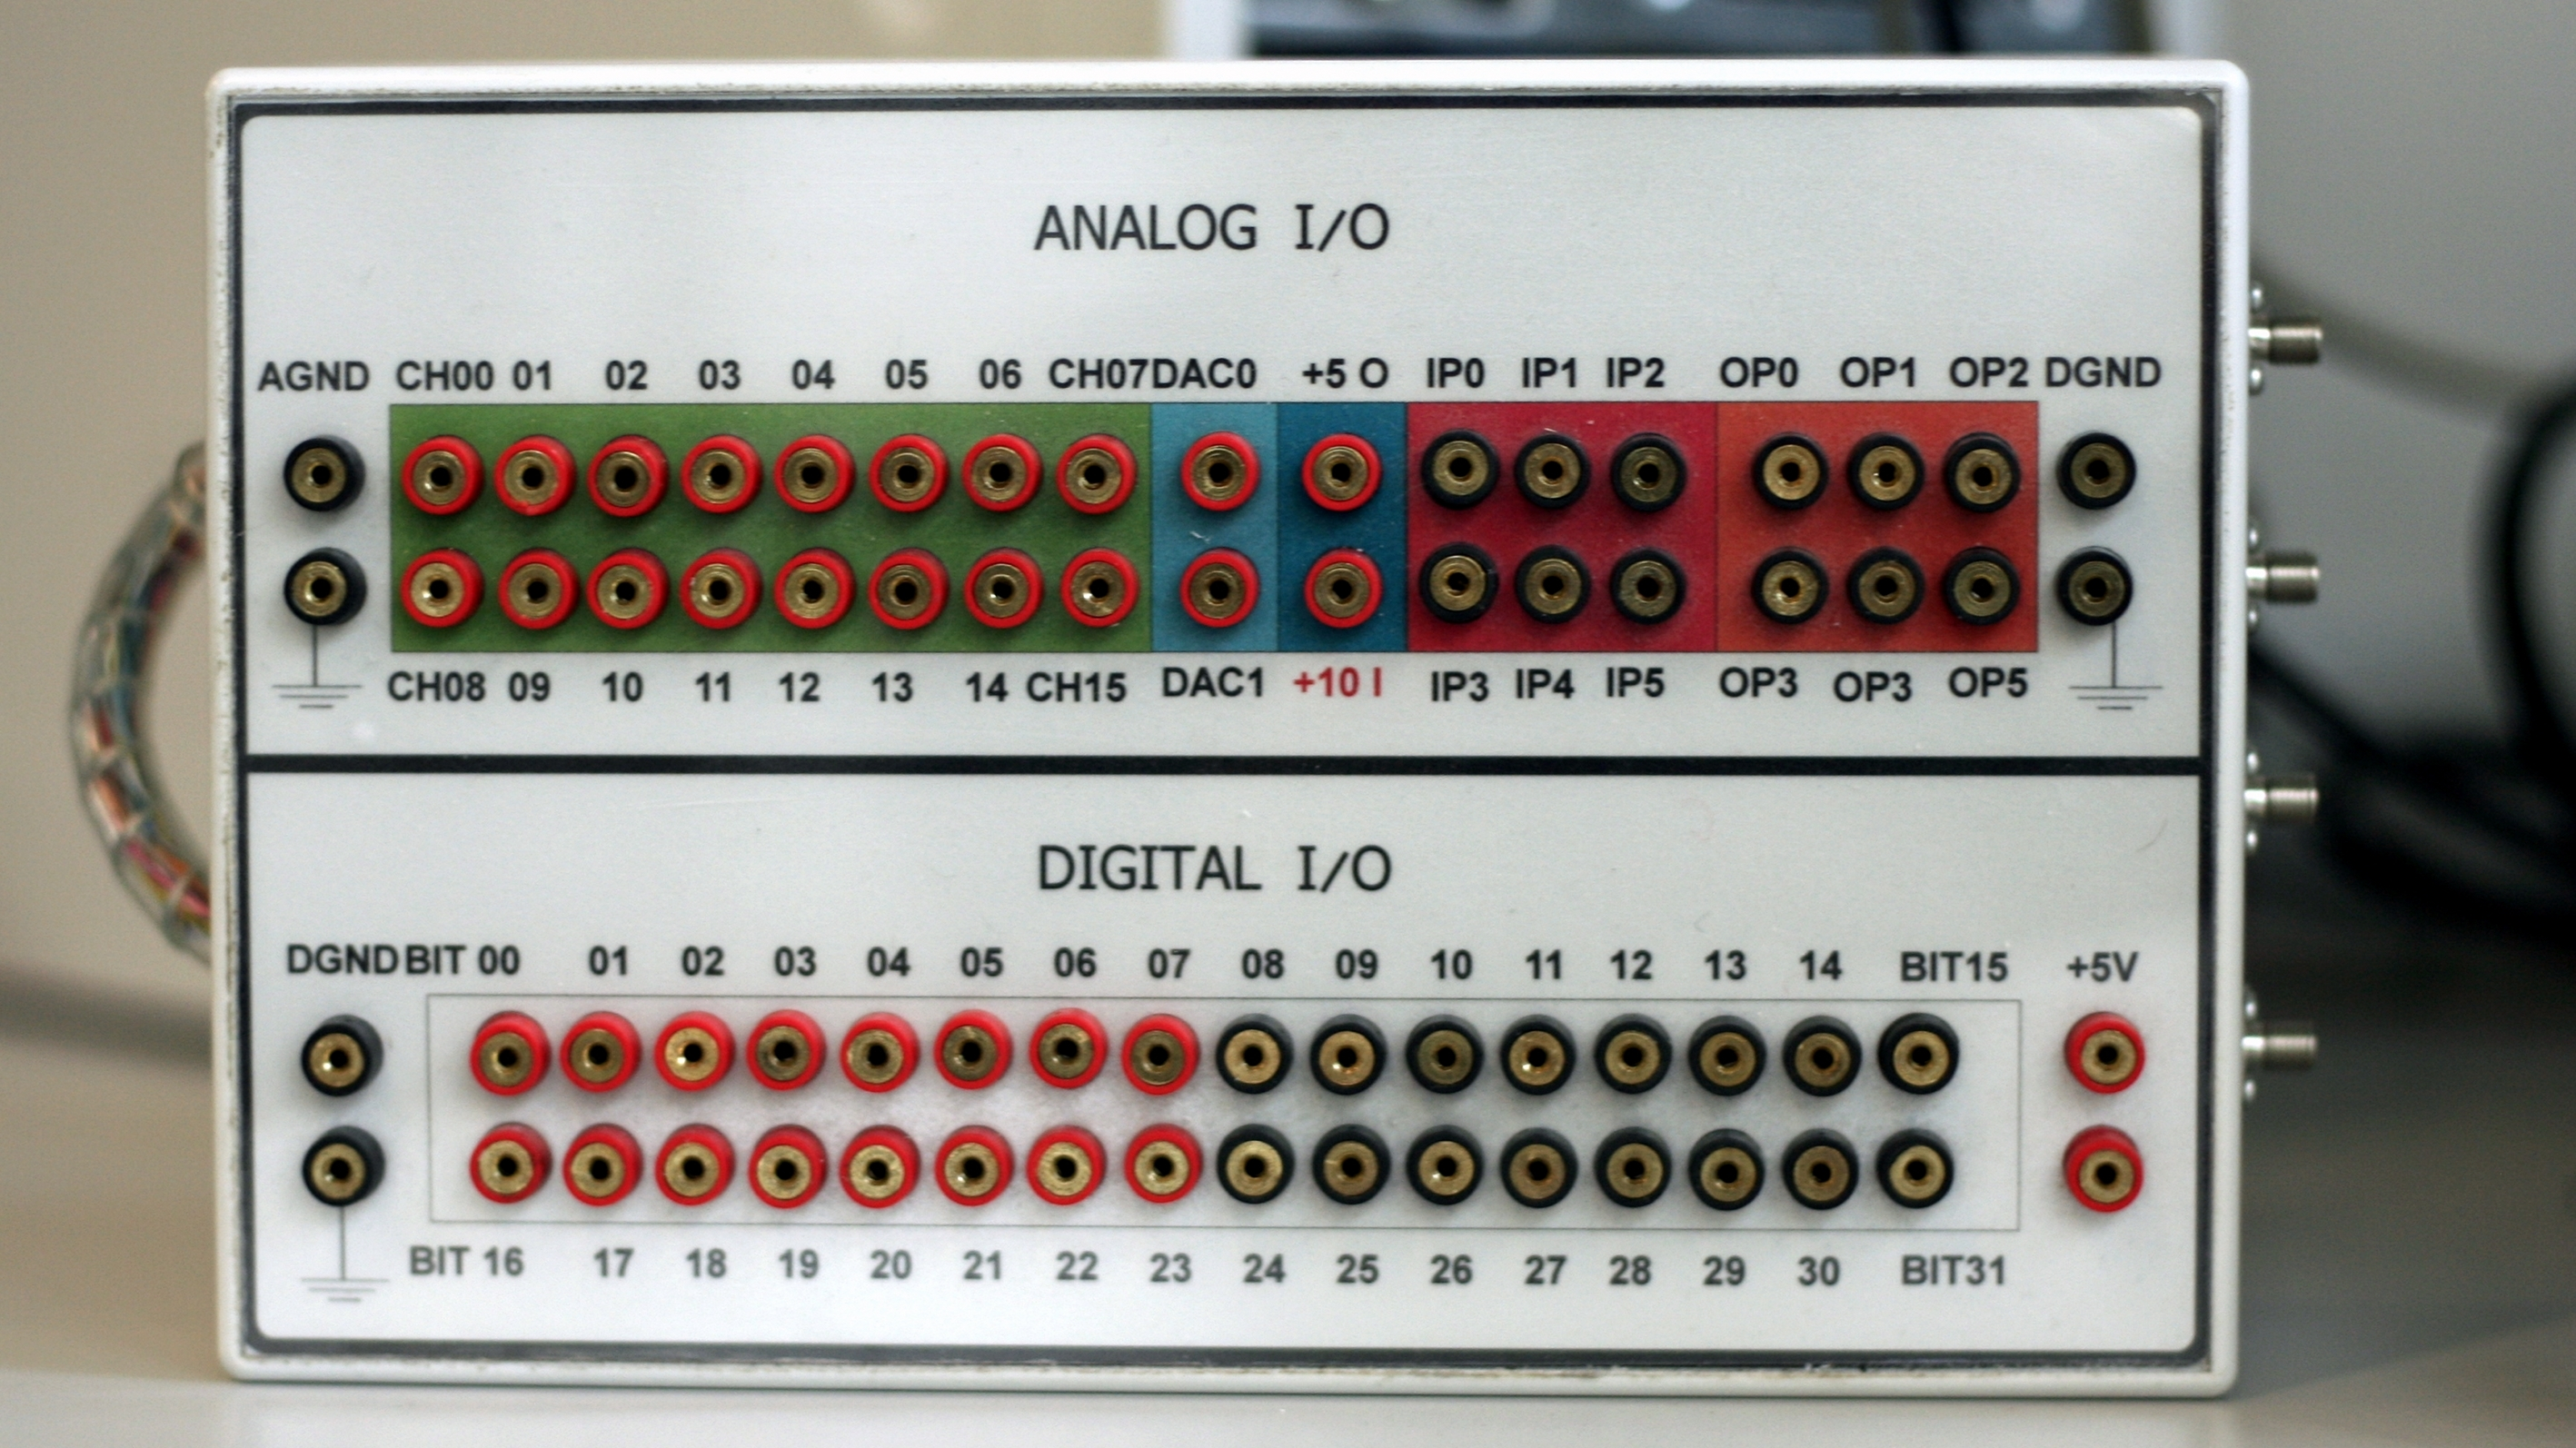
\includegraphics[scale=1, keepaspectratio=true]
		{gis-pfc-ch2-05.jpg}
	\end{center}
	\caption[Plano de la caja de conexiones ya terminada] {Plano de la
	caja de conexiones ya terminada.}
	\label{fig:conbox}
\end{figure}

\chapter{Subsistema de control y presentación}\label{chap:control}

El último de los subsistemas que conforma el sistema de medida digital es
el subsistema de control y presentación. Es el subsistema de más alto nivel
de entre los que integran el sistema por interactuar directamente con el
supervisor. El bloque de control y el bloque de presentación son los que
forman este subsistema y de los que recibe su nombre, la posición relativa
que ocupan éstos con respecto al resto de elementos del sistema de medida
digital puede observarse en la representación parcial que del sistema se
hace en la \vref{fig:subconpre}. Sin embargo, en la práctica estos dos
bloques se mezclan en una misma entidad indivisible, un software que se
ejecuta en el \pc{} anfitrión en el que se encuentra instalada la tarjeta
de adquisición. Por ser el software que gobierna la tarjeta de adquisición
pasa a conocerse en este documento como \emph{software de control}.

\begin{figure}
	\begin{center}
		\includegraphics{gis-pfc-ch3-01.mps}
	\end{center}
	\caption[Subsistema de control y presentación] {Bloques de control
	y presentación dentro del subsistema de control y presentación.}
	\label{fig:subconpre}
\end{figure}

El subsistema de control y presentación constituye la interfaz entre el
supervisor y el sistema de medida, como tal, es una de sus funciones
proporcionar control sobre el sistema al supervisor: ejecutar las órdenes
administradas por el supervisor y gestionar el funcionamiento del resto de
subsistemas. El bloque de control es el encargado de esta actividad y
desempeña las siguientes tareas:

\begin{itemize}
	\item Iniciar y detener la sesión de adquisición.
	\item Interactuar con los drivers de la tarjeta por medio del
		sistema operativo para controlar parámetros de la sesión de
		adquisición como pueden ser, por ejemplo, puertos de
		entrada, modos de adquisición y terminación, o frecuencia
		de muestreo.
	\item Realizar el mantenimiento de los buffers de memoria. Tarea
		que puede dividirse, o consta a su vez, de dos tareas de
		menor complejidad: dar formato a las muestras almacenadas
		en el o los buffers situados en la memoria interna de la
		tarjeta para su comprensión por parte del ordenador
		anfitrión; trasladar las muestras formateadas adecuadamente
		a la memoria del \pc{} para que de ese modo puedan ser
		manipuladas por el usuario administrador.
\end{itemize}

Por su parte, corresponde al bloque de presentación presentar al supervisor
información de utilidad a partir de la señal digital que procede del
subsistema de adquisición. La información debe mostrarse al supervisor para
que pueda interpretarla. En consecuencia, y sometiendo el diseño de la
aplicación de software al criterio del director del PFC, se concluye en
dotar al bloque de presentación con la capacidad de proporcionar la
siguiente información acerca de la señal:

\begin{itemize}
	\item El valor instantáneo cada 250 ms.
	\item El valor medio en el mismo intervalo de tiempo. Este valor
		debe calcularse a partir de las muestras obtenidas en dicho
		periodo a una frecuencia de muestreo que queda a elección
		del supervisor. Debe ser posible seleccionar la frecuencia
		de muestreo desde el propio software de control.
	\item La forma instantánea de la señal, de un fragmento de una
		duración determinada. Debe ser posible también seleccionar
		la duración del fragmento. Simultáneamente debe
		representarse el espectro en frecuencia del fragmento de
		señal que aparece en pantalla.
\end{itemize}

Este capítulo se ha distribuido en dos apartados. En el primero de los
apartados se describe la herramienta empleada en el desarrollo del software
de control. En el segundo se exponen las conclusiones obtenidas al estudiar
el osciloscopio digital como herramienta de referencia en la representación
gráfica de señales. De ese modo se evita explicar el significado del código
correspondiente al software de control línea por línea, puesto que el
lector puede concebir su propia idea del aspecto que adopta el software en
su estadio definitivo de desarrollo. El ejercicio de reflexión pertinente
conduce a una positiva comprensión del proceso que partiendo del diseño
original concluye en el resultado esperado.

% 				( V )
% ______________________________m\"/m______________________________________
%				  '
% El texto comentado aquí abajo debe trasladarse a otra sección del
% capítulo
% _________________________________________________________________________
%
% Se impone una condición de diseño adicional, el software de control debe
% ser poco exigente a fin de que pueda ser ejecutado en un \pc{} que
% disponga de escasos recursos. Para cumplir con dicha condición se propone
% la siguiente solución: limitar la cantidad de datos diferentes
% presentados por pantalla simultáneamente a uno. De ese modo el usuario
% del software debe elegir en cada momento entre el valor instantáneo, el
% valor medio y la forma de la señal y su espectro en frecuencia, y sólo el
% tipo de dato seleccionado se genera reduciendo el coste de procesado.
% Esta solución puede ampliarse incorporando la posibilidad de deshabilitar
% la representación del espectro o de la forma de la señal.
%
% 				 ,._
%				@",_)6
%				 " "

\section{Herramienta de Adquisición de Datos}


\subsection{Introducción}

\psig{matlab} (\emph{MATrix LABoratory}) es la plataforma seleccionada para
el desarrollo del software de control. Es una plataforma de desarrollo bien
conocida en entornos matemáticos y tecnológicos de uso extendido en
universidades y otros centros educativos y de investigación. Encaja en la
descripción de un kit de desarrollo de software (\psig{sdk}) al estar
compuesto por un entorno de desarrollo integrado (\psig{ide}) con editor,
compilador y depurador; y una colección de módulos y extensiones que en
conjunto se comportan como una interfaz de programación de aplicaciones
(\psig{api}).  \matlab{} se caracteriza por emplear un lenguaje propio, el
lenguaje \psig{m}, enfocado a un uso matemático y que se ha diseñado para
simplificar el manejo de datos agrupados en estructuras matemáticas
complejas como son las matrices y los vectores. Los módulos y herramientas
que se incluyen en el \sig{sdk} contribuyen a ampliar su funcionalidad,
convirtiéndolo en un software potente y completo. Estas herramientas
abstraen al desarrollador de implementar por sí mismo en lenguaje \sig{m}
funciones destinadas a realizar operaciones cotidianas como representar
unos datos por pantalla u obtener la \sig{fft} de un vector. Existen
módulos ---o \emph{toolboxes} como se los conoce en inglés--- mantenidos
por la compañía de software, a los que se suman los diseñados por los
propios usuarios, que abundan en la red, disponibles desde la base de datos
dispuesta para ello por la empresa, con lo que las posibilidades son en la
práctica infinitas.  Además \matlab{} cuenta con dos herramientas
fundamentales, muy ligadas al \sig{sdk}, una es \psig{guide}
(\emph{Graphical User Interface Development Environment}), una herramienta
para el desarrollo de interfaces gráficas de usuario (\psig{gui}); y otra
\emph{Simulink}, herramienta que se emplea para realizar todo tipo de
simulaciones.

Las dos razones principales por las que se utiliza \matlab{} son, por un
lado, las facilidades que aporta en la creación de \gui{} y manejo de
señales digitalizadas; y por otro, y aún más importante si cabe, que
incorpora una herramienta denominada \emph{Data Acquisition Toolbox},
nombre que podría traducirse como Herramienta de Adquisición de Datos, en
lo sucesivo \psig{dat}. La \datx{} es una herramienta compuesta por una
biblioteca y un mecanismo para el intercambio de información, que en
conjunto permiten mediante código de alto nivel interactuar directamente
con dispositivos de características similares a las de la tarjeta de
adquisición \kpci{}, y que es convenientemente compatible con ésta tarjeta.
En otras palabras, puede entenderse la \datx{} como una \sig{api} o
interfaz que proporciona al desarrollador las llamadas necesarias para
interactuar directamente con dispositivos de adquisición al tiempo que
abstrae los mecanismos de más bajo nivel que intervienen en el proceso,
descargando al desarrollador de la responsabilidad de implementarlos por él
mismo. Lo que, al fin y al cabo puede resumirse en que en la \datx{} se
implementa el núcleo de lo que se entiende como bloque de control. Al
programarse el software de control empleando los recursos que proporciona
la \datx{}, la herramienta en sí pasa a ser parte fundamental del
subsistema de control y presentación al prestarse como núcleo del bloque de
control. Cobra pues vital importancia en el sistema de medida. En
consecuencia, resulta adecuado un apartado en el que se introduzca la
herramienta al lector. En primer lugar se describen las distintas entidades
que participan en el funcionamiento de la herramienta, justo después se
recoge un subconjunto de las distintas funciones que la \datx{} pone a
disposición del desarrollador ordenadas siguiendo el mismo orden en el que
son requeridas durante la sesión de adquisición de carácter más básico.


\subsection{Componentes de la herramienta}

Los elementos de \matlab{} que juegan un papel suficientemente importante
en el funcionamiento de la \datx{} son los listados en el
\cref{tab:toolcomp}. El diagrama representado en la \vref{fig:toolcomp}
muestra las interdependencias que existen entre los elementos que aparecen
en dicho cuadro.

\begin{table}
	\centering
	\begin{tabulary}{.9\textwidth}{C L}
		\toprule
		Componente & \multicolumn{1}{c}{Propósito} \\
		\midrule
		Ficheros *.m & Se emplean para automatizar la creación de
		objetos dispositivo, adquirir datos, configurar las
		propiedades del dispositivo y la sesión, y evaluar el
		estado de la adquisición y los recursos.\\
		\midrule
		Máquina virtual de adquisición de datos & Almacena objetos
		dispositivo y sus propiedades, controla el almacenamiento
		de los datos adquiridos y controla la sincronización de
		eventos.\\
		\midrule
		Adaptadores & Son la vía de comunicación entre la máquina
		virtual de adquisición de datos y el hardware por la cual
		se transmiten propiedades, datos y eventos.\\
		\bottomrule
	\end{tabulary}
	\caption[Descripción de los componentes de la \datx{}] {Descripción
	de los componentes de la \datx{}.}
	\label{tab:toolcomp}
\end{table}

\begin{figure}
	\begin{center}
		\includegraphics{gis-pfc-ch3-02.mps}
	\end{center}
	\caption[Elementos que intervienen en el proceso de
	adquisición]{Elementos que intervienen en el funcionamiento de la
	\datx{}.}
	\label{fig:toolcomp}
\end{figure}

\subsubsection{Objetos dispositivo}

Los objetos dispositivo permiten el acceso a subsistemas específicos del
hardware. Los objetos dispositivo soportados por la \datx{} son los objetos
de entrada analógica o \emph{analog imput objects} (\psig{ai}), los objetos
de salida analógica o \emph{analog output objects} (\psig{ao}) y los
objetos de entrada/salida digital o \emph{digital I/O objects}
(\psig{dio}).

\begin{figure}
	\begin{center}
		\includegraphics{gis-pfc-ch3-03.mps}
	\end{center}
	\caption[Flujo de información entre el hardware y la
	\sig{dat}]{Grafo que representa la comunicación entre los
	subsistemas del hardware y los objetos dispositivo.}
	\label{fig:subsystemsOO}
\end{figure}


\subsection{La sesión de adquisición de datos}

Una sesión completa de adquisición de datos consiste en cinco pasos:

\begin{enumerate}
	\item Crear el objeto dispositivo.
	\item Añadir canales al objeto dispositivo.
	\item Configurar las propiedades del objeto dispositivo y los
		canales añadidos para controlar el comportamiento de la
		aplicación de adquisición de datos.
	\item Adquirir los datos.
	\item Eliminar el objeto dispositivo.
\end{enumerate}

Cada uno de los pasos se detalla en los puntos subsiguientes.


\subsubsection{Crear el objeto dispositivo}

Para crear un objeto dispositivo, se debe llamar a la función de creación
apropiada o constructor. Como se muestra en el \cref{tab:constructors}, los
constructores reciben un nombre particular en función del tipo de objetos
dispositivo que crean. Para iniciar una sesión de adquisición de datos
analógicos es necesario un comando como el siguiente, \func{analoginput}
\func{(`adaptador', ID)}. Un ejemplo extraído del código fuente de la
aplicación de control muestra cómo hacerlo en el \cref{cod:constructor}.

\begin{table}
	\centering
	\begin{tabular}{l >{\tt}l}
		\toprule
		\multicolumn{1}{c}{Tipo de subsistema} %
		& \multicolumn{1}{c}{\rm Constructor} \\
		\midrule
		Entrada analógica & analoginput(`adaptador', ID); \\
		\midrule
		Salida analógica & analogoutput(`adaptador', ID); \\
		\midrule
		Entrada / Salida digital & digitalio(`adaptador', ID); \\
		\bottomrule
	\end{tabular}
	\caption[Tipos de constructor y objetos dispositivo]{Tipos de
	función de creación de acuerdo con el tipo subsistema al que se
	orienta el objeto dispositivo creado.}
	\label{tab:constructors}
\end{table}

\begin{lstlisting}[style=displayed, caption={[Método a seguir para crear un
	objeto dispositivo] {Método que evalúa la existencia de un objeto
	dispositivo previo a la llamada de la aplicación, en caso positivo
	lo hereda para su uso posterior, de lo contrario crea uno
	nuevo.}}, label={cod:constructor}]
	handles.ai = [];

	if ~isempty(daqfind)
		oldObj = daqfind;

		for i = 1:length(oldObj);
			auxStr = daqhwinfo(oldObj(i));
			auxNum = findstr(' ', ...
				auxStr.DeviceName) - 1;
			if strcmp('KPCI-3108', ...
				auxStr.DeviceName(1:auxNum)) && ...
				strcmpi('analoginput', ...
				auxStr.SubsystemType);
					handles.ai = oldObj(i);
					warning('Device is busy.');
				break
			end
		end

	end

	if isempty(handles.ai)
		try
			handles.ai = analoginput('keithley');
		catch
			errordlg('analoginput function error');
		end
	end
\end{lstlisting}

El argumento \func{id} es un indicador de dispositivo hardware. Se trata de
un argumento opcional para tarjetas de sonido con \func{id} 0. El argumento
\func{adaptador} requiere el nombre del adaptador de dispositivo hardware.
A continuación, en el \cref{tab:adaptors} se muestra una relación con los
adaptadores de dispositivo cuyo uso es más frecuente y el nombre de
adaptador que debe introducirse como argumento de la llamada a
\func{analoginput}. Por conveniencia se ha añadido Keithley a esta lista.

\begin{table}
	\centering
	\begin{tabular}{l >{\tt\qquad}l}
		\toprule
		\multicolumn{1}{c}{Fabricante de Hardware} %
		& \multicolumn{1}{c}{\rm Nombre de adaptador} \\
		\midrule
		Advantech & advantech \\
		\midrule
		Measurement Computing & mcc \\
		\midrule
		National Instruments & nidaq \\
		\midrule
		Parallel port & parallel \\
		\midrule
		Microsoft Windows & winsound \\
		\midrule
		Keithley Instruments, Inc. & keithley \\
		\bottomrule
	\end{tabular}
	\caption[Valores que puede adoptar el argumento
	\func{adaptador}.]{Valores que puede adoptar el argumento
	\func{adaptador} necesario en la llamada a \func{analoginput}.}
	\label{tab:adaptors}
\end{table}


\subsubsection{Añadiendo canales}

Antes de poder utilizarse, deben añadirse canales al objeto dispositivo.
Para ello, debe emplearse la función \func{addchannel}. Puede pensarse en
un objeto dispositivo como un contenedor de grupos de canales y en los
canales añadidos a un objeto dispositivo como un grupo de canales. Si se
desean añadir dos canales al objeto dispositivo \func{objeto} puede
utilizarse la siguiente llamada \func{cans = addchannel(objeto, 1:2);}.


\subsubsection{Configurando propiedades}

Puede controlarse el comportamiento de una sesión de adquisición de datos o
de una aplicación creada con tal propósito configurando las propiedades de
los objetos dispositivo que intervienen en el proceso de adquisición y de
los canales que dicho objeto contiene. Estas son las reglas principales en
la configuración de propiedades desde la \datx{}.

\begin{itemize}
	\item Los nombres de las propiedades pueden escribirse en
		mayúsculas, minúsculas o combinación de ambas.
	\item Los nombres de las propiedades pueden abreviarse como se
		mostrará a continuación. % Hay que confirmar que se
		% explican las reglas de abreviatura
	\item La función \func{set} aplicada a un objeto dispositivo
		---\func{set(objeto)}--- devuelve todas las propiedades
		configurables de ese objeto. Si se llama a \func{set}
		utilizando como argumento un canal ---\func{set(objeto.}
		\func{.Channel(índice)}---, la función devolverá todas las
		propiedades configurables de dicho canal.
	\item La función \func{get} devuelve todas las propiedades de un
		canal u objeto y el valor que toman en el momento en el que
		se llama a la función si se emplea como único argumento
		dicho canal u objeto ---\func{get(objeto)},
		\func{get(objeto.Channel(índice)}---.  \end{itemize}

Se distinguen dos tipos de propiedades distintas asociadas a los canales
contenidos en un objeto dispositivo.

\begin{description}
	\item[Propiedades comunes] Son aquellas propiedades que se aplican
		todos los canales pertenecientes a un mismo objeto
		dispositivo.
	\item[Propiedades de canal] A diferencia de las propiedades
		comunes, las propiedades de canal pueden configurarse
		individualmente por canal.
\end{description}

Dentro de las propiedades comunes de los canales existen las
\emph{propiedades básicas}, que se aplican a todos los subsistemas de un
determinado tipo (\textsc{ai, ao, dio}); y \emph{propiedades específicas de
dispositivo} aplicables únicamente al hardware específico que se está
empleando.

Existen tres formas de configurar u obtener el valor de una propiedad:
utilizando las funciones \func{set} y \func{get}; empleando la notación de
punto; o recurriendo a los nombres indexados.

\begin{itemize}
	\item La sintaxis de las funciones \func{get} y \func{set} es
		similar a la empleada en la herramienta de \matlab{}
		\emph{Handle Graphics}.

		\begin{lstlisting}[gobble=16]
			out = get(objeto, `SampleRate');
			set(objeto, `SampleRate', 11025)
		\end{lstlisting}

	\item La notación de punto se emplea del siguiente modo:

		\begin{lstlisting}[gobble=16]
			out = objeto.SampleRate;
			objeto.SampleRate = 11025;
		\end{lstlisting}

	\item Por último, los nombres indexados permiten asociar un nombre
		descriptivo a cada canal. Por ejemplo para asociar el
		nombre \func{Can1} con el primer canal contenido en
		\func{objeto} debe procederse como se enuncia a
		continuación.

		\begin{lstlisting}[gobble=16]
			set(objeto.Channel(1), `ChannelName', ...
				`Can1');
			out = objeto.Can1.UnitsRange;
			objeto.Can1.UnitsRange = [0, 10];
		\end{lstlisting}

\end{itemize}


\subsubsection{Adquisición de datos}

La adquisición de datos puede dividirse en tres tareas básicas: iniciar el
objeto dispositivo; registrar datos y detener el objeto dispositivo.

La función que se utiliza para iniciar un objeto dispositivo es la función
\func{start}, p.e. para iniciar el objeto dispositivo \func{objeto} habría
que llamar a la función de esta forma \func{start(objeto)}. Tras iniciar un
objeto su propiedad \textsf{Running} pasa de manera automática al valor
\textsf{On}.

No obstante haber iniciado el dispositivo, este no empieza a registrar
datos hasta que no ocurre un trigger o disparo. Hay diversos tipos de
trigger, en el \vref{tab:triggers} se muestran aquellos soportados por
todos los dispositivos. Tras un trigger el dispositivo hardware inicia la
adquisición de datos y la propiedad \textsf{Logging} del objeto dispositivo
asociado conmuta al estado \textsf{On}.

\begin{table}
	\centering
	\begin{tabulary}{.9\linewidth}{>{\sf}c L}
		\toprule
		{\rm Tipo de disparo} & \multicolumn{1}{c}{Descripción} \\
		\midrule
		Inmediato & El disparo ocurre justo después de la llamada a
		\func{start}. Este es el tipo de trigger predeterminado. \\
		\midrule
		Manual & El disparo ocurre después de llamar manualmente a
		la función \func{trigger}. \\
		\midrule
		Software & El disparo sucede cuando se detecta una señal
		que satisface una determinada condición especificada de
		antemano. El objeto dispositivo debe disponer de más de un
		canal que hará las veces de la señal de disparo. Debe
		especificarse, como es obvio, que canal actúa como fuente
		del disparo. \\
		\midrule
		Reloj interno & Por añadidura, la \kpci{} cuenta con la
		posibilidad de recibir el disparo de la fuente de reloj
		interna. \\
		\bottomrule
	\end{tabulary}
	\caption[Tipos de disparo soportados]{Tipos de disparo soportados
	por el hardware compatible con \matlab{} y una breve descripción de
	los mismos.}
	\label{tab:triggers}
\end{table}

Por último, existen tres causas por las que un objeto dispositivo puede
detenerse: \matlab{} detiene un objeto dispositivo iniciado una vez
obtenidos los datos precisados por el usuario; al ocurrir un error de
tiempo de ejecución en relación con la actividad de un objeto dispositivo
éste es detenido también; y tan sólo resta el método manual, que consiste
en llamar a la función \func{stop}, por ejemplo \func{stop(objeto)}.

Como se ha mencionado la máquina virtual de adquisición de datos registra y
controla los datos que extrae de un objeto dispositivo. Un usuario puede
acceder a esos datos de dos formas diferentes:

\begin{itemize}
	\item La primera de ellas se conoce como previsualizar los datos.
		Se emplea con ese propósito la función \func{peekdata}. Si,
		por ejemplo, se quisiese previsualizar 1000 muestras
		obtenidas con el objeto dispositivo \func{objeto}, la
		llamada a \func{peekdata} sería la siguiente: \func{out =
		peekdata(objeto, 1000);}. La función \func{peekdata}
		devuelve el control a \matlab{} de inmediato y no elimina
		los datos previsualizados de la máquina virtual de
		adquisición.
	\item En cualquier momento tras adquirir datos mediante un objeto
		dispositivo estos pueden extraerse de la máquina virtual de
		adquisición mediante la función \func{getdata}. Partiendo
		del ejemplo anterior, si se desea extraer 1000 muestras
		procedentes del objeto dispositivo \func{objeto}, esta es
		la llamada adecuada \func{out = getdata(objeto, 1000);}. Al
		contrario que la función \func{peekdata}, \func{getdata} no
		devuelve el control a \matlab{} hasta haber extraído todas
		las muestras solicitadas. Es evidente que las muestras
		extraídas dejarán de estar disponibles en la máquina
		virtual de adquisición.
\end{itemize}

Es importante señalar que en cualquiera de los procedimientos descritos
intentar acceder a más datos de los obtenidos en un determinado momento
causará un error que detendrá el funcionamiento del objeto dispositivo.


\subsubsection{Eventos y Callbacks}

Puede decirse que un evento sucede en un determinado instante después de
que una cierta condición se cumple. A menos que ocurra un error, en todas
las sesiones de adquisición de datos debe producirse un evento de inicio,
uno de disparo y uno de parada. Puede accederse a la información que
transporta un evento mediante la propiedad \textsf{EventLog}:

\begin{lstlisting}
	Events = ai.EventLog;
	EventTypes = {Events.Types}
	EventTypes =
		`Start'    `Trigger'	`Stop'
\end{lstlisting}

Cuando se produce un evento, puede ejecutarse una función de
\emph{callback}. Es posible seleccionar una función para un callback
especificando como valor de la propiedad asociada a dicho callback el
nombre de la función (si ésta se encuentra en el mismo fichero *.m que
contiene el código que ejecuta la aplicación que realiza la adquisición de
datos), o el nombre del fichero *.m con el código de la función. Así mismo,
pueden pasarse argumentos de entrada a la función de callback asignándolos
a la mencionada propiedad.

Por ejemplo, los siguientes comandos configuran \func{objeto} de forma que
la función \func{datadqcallback} se ejecute desde el fichero cuyo nombre
está compuesto por una raíz idéntica al nombre de la función y con
extensión *.m, cuando se produzca un evento de trigger o de parada durante
la actividad del objeto dispositivo. Además se pasa como argumento de la
función el valor de la propiedad \textsf{Running} de \func{objeto} en el
momento del callback.

\begin{lstlisting}
	set(objeto, `TriggerFcn', ...
		@datadqcallback, objeto.Running)
	set(objeto, `StopFcn', ...
		@datadqcallback, objeto.Running)
\end{lstlisting}

Un segundo ejemplo, este extraído del código fuente de la aplicación de
control muestra como pasar argumentos a la función de callback y cuál es la
sintaxis de la definición de la misma en el \cref{cod:callback}.

\begin{lstlisting}[style=displayed, caption={[Configuración de
	\emph{callback}]{Configuración de \emph{callback} para responder a
	eventos en la sesión de muestreo, la función de \emph{callback}
	recibe un argumento.}}, label={cod:callback}]
	set(handles.ai, 'TriggerType', ...
		'Immediate', 'TimerFcn', '', ...
		'SamplesAcquiredFcn', ...
		{@localDaqCallback, gcbo});

				[...]

	function localDaqCallback(obj, event, hObject)
		handles = guidata(hObject);
		EventType = event.Type;

		switch lower(EventType)
			case 'samplesacquired'

				[...]

			case 'timer'

				[...]

		end
\end{lstlisting}

\subsubsection{Suprimiendo y borrando las trazas de los objetos dispositivo}

La función \func{delete} elimina el objeto dispositivo especificado de la
máquina virtual de adquisición, pero no del espacio de trabajo (espacio
reservado a las variables de trabajo) de \matlab{},
---\func{delete(objeto)}---. Tras una llamada semejante \func{objeto} sigue
apareciendo en el espacio de trabajo de \matlab{}, pero se trata de un
objeto inválido desde el momento en el que deja de encontrarse ligado al
hardware. Deben suprimirse los objetos dispositivo faltos de validez con el
comando \func{clear}, p.e., \func{clear objeto}.

Si se suprime un objeto dispositivo del espacio de trabajo de \matlab{} no
deja de existir en la máquina virtual. Para poder recuperar objetos
borrados accidentalmente puede utilizarse la función \func{daqfind}.

\begin{lstlisting}
	out = daqfind;		ai = out(1);
\end{lstlisting}


\section{Diseño conceptual del software}\label{sec:softdesign}

\textsc{Matlab} y la \datx{} simplifican en gran medida la tarea de
implementar el bloque de control y la interfaz gráfica de usuario, por
tanto, el último reto importante que debe afrontarse en el desarrollo del
software de control es programar el mecanismo mediante el cual ha de
representarse la señal en pantalla. Es sencillo mostrar por pantalla datos
numéricos o representar la \sig{fft} de una señal gracias a las utilidades
de que dispone \matlab{}, representar una señal en <<tiempo real>> es algo
más complejo. Al fijar los objetivos del \sig{pfc} se especifica que debe
poder utilizarse el sistema de medida para visualizar señales como si se
tratase de un osciloscopio digital. La principal complicación que existe al
programar un osciloscopio digital en software radica en definir las metas
de programación y no en escribir el código. Esto sólo puede lograrse tras
estudiar en profundidad el modelo, después de comprender perfectamente su
comportamiento y de ese modo poder traducir sus principales rasgos de
conducta en metas sencillas. En este apartado se exponen brevemente las
conclusiones extraídas tras estudiar el osciloscopio digital como modelo
para el software de control.


\subsection{El osciloscopio digital}\label{subsec:digosc}

El osciloscopio digital es un dispositivo que se emplea para visualizar
señales, es el sucesor de otros instrumentos como el oscilógrafo y el
osciloscopio analógico. Algo importante a tener en cuenta cuando se estudia
el osciloscopio digital es que se ha diseñado para conseguir un resultado
similar al que se espera de un osciloscopio analógico. La diferencia entre
uno y otro reside en la forma en la que se genera un barrido, el
osciloscopio analógico dibuja la señal sobre la marcha mientras que el
osciloscopio digital digitaliza y almacena la señal digital en memoria
antes de representar. Un barrido es básicamente una imagen de la señal que
abarca toda la pantalla del osciloscopio, se llama así porque el haz de
electrones que emite el tubo de rayos catódicos de un osciloscopio
analógico barre literalmente el monitor para formar la imagen (que no es
más que la imprenta dejada en el monitor por la acción del fósforo). Pero
en los osciloscopios digitales no hay barridos como tal, en realidad los
osciloscopios digitales utilizan monitores \sig{led} en los que los
distintos puntos de luz se apagan, o se encienden, o cambian de color,
accionados por una señal de control. Cuando muchos barridos se suceden
rápidamente se crea la sensación de que la representación de la señal se
mueve, aunque no es así, y en los osciloscopios digitales la representación
es estrictamente estática. Pero el resultado final es muy similar, a
efectos prácticos es el mismo, pues el ojo humano no es capaz de percibir
la diferencia y eso en la práctica significa que esa diferencia no existe.

Pero si existe diferencia, y esa diferencia se nota en algunos aspectos
relacionados con el funcionamiento del osciloscopio digital. Usualmente
tanto los osciloscopios digitales como los analógicos hacen barridos
disparados de la señal, esto es, empiezan a representar la señal al
detectar un evento ---un flanco de subida o de bajada o similar--- en una
señal de referencia que puede y acostumbra a ser la propia señal con la que
se trabaja. De esa forma se consigue alinear todas las capturas o ciclos de
la señal en fase unos con otros y con la señal. Si no se dispara resulta
muy difícil observar la señal con el osciloscopio, especialmente si se
trata de una señal aperiódica, porque los distintos ciclos representados se
superponen y es difícil distinguir la señal correctamente. La diferencia
entre los osciloscopios analógicos y digitales se manifiesta especialmente
en que el osciloscopio analógico empieza a representar la señal cuando
detecta el evento y el usuario puede ver como evoluciona, sin embargo, el
osciloscopio digital empieza a \emph{muestrear} cuando observa el evento y
no representa hasta que tiene muestras suficientes como para abarcar toda
la dimensión temporal representada en el monitor, es ahí donde se hace
evidente un retardo. Imagínese la siguiente situación por ejemplo: se
trabaja con una señal que oscila lentamente y se configura la escala
temporal del osciloscopio para poder observar un periodo completo de la
señal en pantalla, como la señal es lenta su periodo es largo, entonces
llega el evento y en el osciloscopio analógico empieza a verse la señal
apareciendo lentamente desde el margen izquierdo de la pantalla, sin
embargo, en el osciloscopio digital no se ve nada y el retardo se hace
visible y molesto. El retardo que se produce en situaciones como la
expuesta, en las que trata de observarse evoluciones lentas de una señal,
dificulta el uso de los osciloscopios, pero especialmente el uso de los
osciloscopios digitales.

Para paliar los efectos del retardo, el osciloscopio digital aprovecha que
puede representar los datos que tiene en memoria de otras formas diferentes
y, cuando la escala temporal de la representación se configura por encima
de un nivel de umbral, simula el comportamiento de los osciloscopios
analógicos. En lugar de hacer barridos de la señal, actualiza la pantalla
en ciclos cortos añadiendo a la representación fragmentos muy pequeños de
señal, cortos en comparación con la dimensión temporal representada en el
eje de abscisas. Los fragmentos tienen una duración igual al periodo con el
que se refresca el monitor, que es un periodo de refresco fácilmente
asumible por el osciloscopio dada la configuración de la escala temporal,
pero que es muy difícil de seguir por parte del ojo humano. Cuando opera de
este modo, el osciloscopio digital simula que la señal va desplazándose de
derecha a izquierda, y el resultado es idéntico al que muestran los
osciloscopios digitales. Las
\vref{fig:sigmodcont,fig:firmodcont,fig:desmodcont} ilustran este
comportamiento.

\begin{figure}
	\begin{center}
		\includegraphics{gis-pfc-ch3-04.mps}
	\end{center}
	\caption[Señal analógica, representación continua]{Señal analógica
	vista desde la sonda del osciloscopio, se han marcado los instantes
	en los que se refresca el monitor del osciloscopio.}
	\label{fig:sigmodcont}
\end{figure}

\begin{figure}
	\begin{center}
		\includegraphics{gis-pfc-ch3-05.mps}
	\end{center}
	\caption[Evolución que sufre la representación]{Evolución de la
	representación cuando aún no abarca la dimensión horizontal del
	monitor.}
	\label{fig:firmodcont}
\end{figure}

\begin{figure}
	\begin{center}
		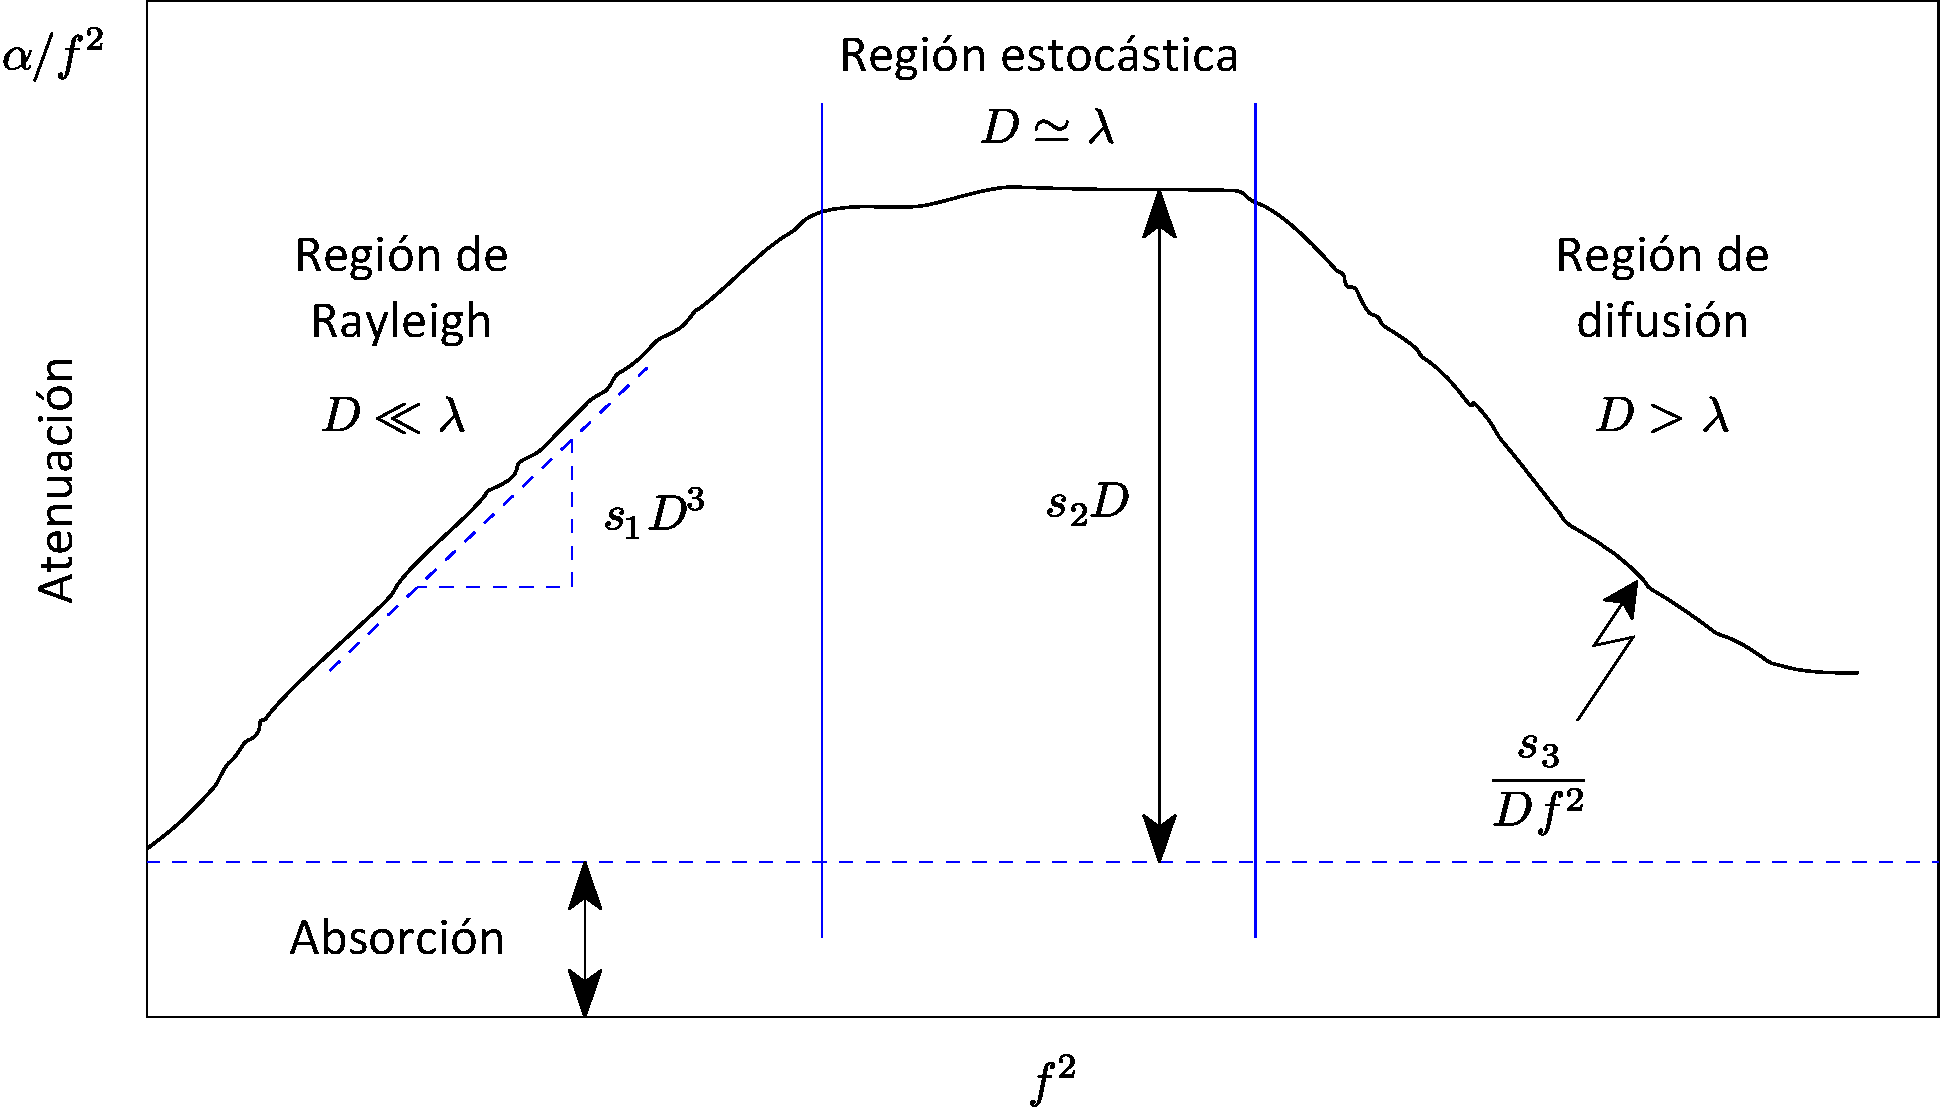
\includegraphics{gis-pfc-ch3-06.mps}
	\end{center}
	\caption[Desplazamiento que experimenta la
	representación]{Desplazamiento que experimenta la representación
	una vez ocupa toda la pantalla del osciloscopio.}
	\label{fig:desmodcont}
\end{figure}

\subsubsection{Barrido disparado}

Implementar un barrido disparado mediante software directamente en la
aplicación de control es complicado teniendo en cuenta la configuración del
sistema de medida. Podría hacerse por hardware, sería necesario generar una
señal de reloj mediante un circuito externo. El circuito requiere de tres
componentes, uno que genera un tren de pulsos rectangulares de frecuencia
100 kHz que se activa y se detiene por flanco de bajada o subida y que
marca el muestreo, otro que genera el flanco que activa el tren de pulsos
cuando la señal de trabajo efectúa una transición de tensión negativa a
tensión positiva y, por último, otro que genera el flanco que detiene el
tren de pulsos. Como señal que detiene el tren de pulsos es necesario un
tren de flancos, pulsos estrechos, cuyo periodo depende de la escala
temporal de la ventana donde se representa la señal. Dependiendo de la
configuración de este parámetro puede cambiarse el valor de tensión que
sale por uno de los puertos de salida analógica de la \kpci{}, y en función
de esta tensión generar una señal en la que el ciclo de trabajo varía y la
duración del estado alto se mantiene. El flanco que detiene el muestreo
puede monitorizarse para averiguar cuando debe la aplicación extraer las
muestras del buffer de memoria asociado a la tarjeta y debe empezar a
procesarlas. La señal de reloj debe pasarse a la tarjeta por el puerto
\textsc{j1}, puerto que puede utilizarse como fuente de reloj hardware
externo, y debe configurarse la tarjeta apropiadamente mediante las
propiedades del objeto dispositivo correspondiente en \matlab{}.

Diseñar el circuito y realizar la configuración correspondiente requiere de
un gran esfuerzo por lo que el problema de implementar barridos por disparo
en el software de control se ha atajado empleando una solución aproximada.
En lugar de empezar a muestrear a partir de un evento, de un pulso o de un
flanco en una señal auxiliar o en la propia señal, se muestrea la señal, y
cuando ha transcurrido el suficiente tiempo como para disponer de bastantes
muestras como para cubrir dos ventanas temporales (en este documento se
llama ventana temporal al tiempo que representa el eje de tiempos en cada
momento), entonces se procesan las muestras y además de eliminar la
componente en continua se detectan los nulos de la señal. Después se alinea
el más próximo de los nulos a la muestra central del intervalo con el cero
del plano cartesiano. De esa forma todas las capturas de la señal aparecen
alineadas. Las \cref{fig:sigmodtri,fig:repmodtri} muestran cual es el
resultado de utilizar este algoritmo.

\begin{figure}
	\begin{center}
		\includegraphics{gis-pfc-ch3-07.mps}
	\end{center}
	\caption[Representación de barridos por disparo]{En esta figura se
	muestran las distintas ventanas que intervienen en la solución
	aproximada utilizada para implementar la representación de barridos
	activados por disparo en el software de control. Puede apreciarse
	la información que se descarta en cada ciclo.}
	\label{fig:sigmodtri}
\end{figure}

\begin{figure}
	\begin{center}
		\includegraphics{gis-pfc-ch3-08.mps}
	\end{center}
	\caption[Representación del fragmento de señal]{Fragmento de señal
	representado centrado en el cero del plano cartesiano.}
	\label{fig:repmodtri}
\end{figure}

El coste que se deriva de utilizar un algoritmo como este para obtener
barridos disparados de la señal es la información que se descarta en cada
ciclo, al desplazar la señal todo lo que queda fuera de la ventana no se
representa, con lo que parte de la información capturada es descartada. En
la \cref{fig:sigmodtri} puede observarse el instante $t_0$, instante en el
que empieza el proceso de adquisición, el instante $t_0 + T$ que representa
el momento en el que este proceso termina. Por tanto, el fragmento de señal
contenido entre estos dos instantes se encuentra digitalizado y almacenado
en memoria en el momento en que empiezan a procesarse las muestras,
inmediatamente después de $t_0 + T$. Sin embargo, después de desplazar la
señal todo aquello que queda fuera de la ventana temporal se descarta y
nunca llega a representarse. Además durante el tiempo en el que el software
procesa y representa la señal digital, desde $t_0 + T$ hasta $t_1$, no se
muestrea, por lo que el fragmento de señal que transcurre en esos instantes
también pasa inadvertido al usuario. Todo ello puede contribuir a que
ciertos eventos ocurridos en la señal se pierdan ocasionalmente, sin
embargo, esta solución ha dado hasta el momento muy buenos resultados, tal
y como se demuestra en el \cref{chap:part1conclusions}.

\chapter{Resultados y conclusiones}\label{chap:part1conclusions}

Para poder valorar la utilidad real de la aplicación frente a los distintos
dispositivos ya disponibles y que realizan una función semejante se ha
decidido comparar los resultados que se obtienen al utilizar la tarjeta y
un osciloscopio, como elemento representativo, en una prueba genérica.

Por separado, se ha evaluado el rendimiento del subsistema de interacción
con el medio físico (el conjunto formado por los circuitos acondicionadores
y los transductores de ultrasonidos).


\section{Objetivos}

El objetivo de la prueba de rendimiento es determinar las prestaciones y
limitaciones del sistema de medida desarrollado. Para ello se han comparado
los resultados obtenidos al visualizar una batería de señales en un
osciloscopio de laboratorio y en el sistema de medida. Los parámetros que
se han evaluado son los siguientes.

\begin{itemize}
    \item Medida en tiempo real de la amplitud de la señal en ambos
	dispositivos.
    \item Medida en tiempo real de la frecuencia de la onda eléctrica.
    \item Fidelidad de la representación.
    \item Capacidad para seguir la forma de la onda en el modo continuo de
	representación.
\end{itemize}

Se ha realizado además una prueba secundaria para poder determinar que las
funciones de la aplicación de control operan satisfactoriamente.


\section{Metodología}\label{sec:working-test}

El procedimiento de medida consta de unos sencillos pasos. Previamente a la
realización de las observaciones se dispone el equipo. El equipo utilizado
está formado por los siguientes elementos:

\begin{itemize}
    \item Generador de señales, utilizado para generar la distintas señales
	utilizadas para las pruebas.
    \item Osciloscopio, en el que se observa la representación que sirve de
	referencia para la comparación.
    \item Un equipo (\pc{}) en el que se encuentran previamente instaladas
	la tarjeta de adquisición y la aplicación de control.
    \item La caja de conexiones desarrollada para la tarjeta de
	adquisición (\vref{fig:conbox}).
    \item Sondas terminadas en ambos extremos con conectores de tipo banana
	compatibles con la caja de conexiones.
    \item Sondas para el osciloscopio y el generador de señales.
\end{itemize}

Los pasos seguidos para evaluar la bondad de la representación en el
sistema de medida se enumeran a continuación.

\begin{enumerate}
    \item Se lanza la aplicación de control.
    \item Se configura el osciloscopio para que proporcione una medida de
	la amplitud de la señal en Vpp y de su frecuencia.
    \item Se selecciona una forma de onda en el generador de señales.
    \item Para la onda seleccionada se elige una amplitud 16 Vpp.
    \item Se selecciona la frecuencia más baja del rango expuesto en el
	\cref{tab:testparameters}.
    \item Se observa la señal representada en el osciloscopio y en el
	sistema de medida, comparando si la segunda es fiel a la primera.
	Se anotan los valores observados de amplitud y frecuencia en ambos
	dispositivos.
    \item Se repiten los pasos desde el paso 5 hasta agotar todas las
	frecuencias. Después se selecciona una frecuencia fija de 1 kHz y
	se repite el procedimiento para distintos valores de amplitud.
    \item Se repite todo el procedimiento desde el tercer paso hasta haber
	completado la prueba para todos los tipos de señal evaluados.
\end{enumerate}

Cabe mencionar que mientras que el osciloscopio proporciona automáticamente
un valor de frecuencia y uno de amplitud para cada señal evaluada, en el
sistema de medida es preciso determinar esos valores a partir de la señal
representada (amplitud) y su espectro en frecuencias (frecuencia central).

El \cref{tab:testparameters} muestra los parámetros de la prueba: los
distintos tipos de señal evaluados; los valores de frecuencia y los valores
de amplitud.

\begin{table}
    \centering
    \begin{tabular}{l d{5.1}d{8.1}d{2.1}}
	\toprule
	& \multicolumn{3}{c}{Parámetros de la señal} \\
	\cmidrule(l){2-4}
	Tipo de señal & \multicolumn{1}{c}{Frecuencia (Hz)} &
	    \multicolumn{1}{c}{Periodo ($\mu\text{s}$)} &
	    \multicolumn{1}{c}{Amplitud (Vpp)} \\
	\midrule
		    & 0,1	& 10000000	& \\
		    & 1		& 1000000	& \\
	Sinusoidal  & 5		& 2000000	& 16 \\
		    & 25	& 40000		& \\
	Rectangular & 1000	& 10000		& 10 \\
		    & 1000	& 10000		& \\
	Triangular  & 10000	& 100		& 1 \\
		    & 20000	& 50		& \\
	Pulsada	    & 30000	& 33,3		& 0,1 \\
		    & 40000	& 25		& \\
		    & 50000	& 20		& \\
	\bottomrule
    \end{tabular}
    \caption[Parámetros de la prueba]{Parámetros de la prueba.}
    \label{tab:testparameters}
\end{table}


\subsection{Procedimiento, prueba secundaria}

El objetivo de la prueba secundaria es el de establecer que las distintas
funciones implementadas en la aplicación de control realizan su cometido
satisfactoriamente. Para la realización de esta prueba se ha empleado el
mismo equipo que en la prueba principal. El procedimiento que se ha seguido
consta de una serie de pasos que se enumeran a continuación.

\begin{enumerate}
    \item Tras disponer el equipo y conectar los dispositivos se ajusta el
	generador de señales para que transmita una onda sinusoidal de 1 Hz
	de frecuencia y una amplitud de 1 Vpp.
    \item Se comprueba que las medidas numéricas se correspondan con lo
	esperado.
    \item Después se ajusta la frecuencia de muestreo y la ganancia del
	amplificador interno de la tarjeta de adquisición y se comparan los
	resultados.
    \item La sonda que transmite la señal al sistema de medida se conecta a
	cada puerto de entrada y se evalúa que estos funcionan
	correctamente. Para ello se selecciona cada vez el canal adecuado
	en la aplicación de control.
    \item Se ajusta el generador de señales para que transmita esta vez una
	señal de 4 kHz y 16 Vpp.
    \item Se evalúan las distintas opciones del modo gráfico de
	funcionamiento: selección de la escala temporal, selección de la
	escala de amplitud, selección del número de puntos para la
	realización de la \sig{fft}, representación de la señal y su
	espectro en frecuencias en la ventana de representación elegida,
	habilitación o inhabilitación de alguna o ambas representaciones.
\end{enumerate}


\section{Resultados}

Dada la multitud de variables que intervienen en la realización de las
pruebas se obtiene una gran cantidad de resultados, en este documento se ha
optado por ofrecer sólo una muestra representativa de los mismos
(\cref{tab:measureresults}).

\begin{table}
    \centering
    \begin{tabular}{ld{2,1}d{2,4}}
	\toprule
	& \multicolumn{2}{c}{Valores en el sistema} \\
	\cmidrule(r){2-3}
	Señal evaluada & \multicolumn{1}{c}{amplitud (Vpp)} &
	    \multicolumn{1}{c}{frecuencia (kHz)} \\
	\midrule
	sinosoidal @ 16 Vpp, 1 Hz & 16 & ~1 Hz \\
	sinosoidal @ 16 Vpp, 5 Hz & 16 & 5 Hz \\
	sinosoidal @ 0,1 Vpp, 10 kHz & 0,1 & 9,9 \\
	sinosoidal @ 16 Vpp, 10 kHz & 16 & 10 \\
	rectangular @ 16 Vpp, 10 kHz & 16 & 9,5 \\
	triangular @ 16 Vpp, 10 kHz & 15,4 & 9,35 \\
	pulsada @ 16 Vpp, 10 kHz & 15,3 & 9,35 \\
	sinosoidal @ 16 Vpp, 20 kHz & 16 & 20 \\
	sinosoidal @ 16 Vpp, 40 kHz & 16 & 40 \\
    \end{tabular}
    \caption{Resultados obtenidos, se ha omitido la columna correspondiente
    al osciloscopio.}
    \label{tab:measureresults}
\end{table}


\subsubsection{Observaciones}

Complementando los resultados expuestos en el \cref{tab:measureresults} se
hacen las siguientes observaciones sobre la fidelidad de la representación.

A frecuencias por debajo de 1 Hz el disparo del sistema empieza a fallar
(del mismo modo que ocurre en los osciloscopios), por lo que se hace
necesario representar la señal en modo continuo. Se ha observado que en
sistemas con un rendimiento gráfico bajo la representación de la señal
vista en el sistema de medida cuando representa en modo continuo no
consigue seguir a la señal, pueden verse escalones correspondientes al
instante en el que el búffer de la aplicación se refresca.

Por otro lado, al ser limitada la frecuencia de muestreo del dispositivo de
adquisición, la representación de la señal empieza a perder forma (aunque
se siguen observando valores correctos de amplitud y frecuencia) a partir
de los 25 kHz aproximadamente.

Por último se ha advertido que la caja de conexiones presenta un fallo.
Cuando se inserta señal a través de un puerto analógico parte de esa señal
se observa se resta en el resto de puertos de la misma fila (existen dos
filas de puertos, una del 0 al 7 y otra del 8 al 15). Ello impide que se
puedan utilizar dos puertos de la tarjeta simultáneamente (se subraya que
es un fallo de la caja de conexiones y no de la aplicación de control).


\subsection{Resultados, prueba secundaria}

Las pruebas realizadas determinan que la aplicación de control no está
afectada por ningún defecto de funcionamiento excepto por los observados en
este apartado.

Las imágenes expuestas a continuación en las
\crefrange{fig:default}{fig:point-number} muestran que los controles que
regulan el comportamiento del modo gráfico de funcionamiento realizan su
función satisfactoriamente. Sin embargo se observa un fallo de
funcionamiento probablemente debido al equipo en el que se han desarrollado
las pruebas: en ocasiones al lanzar la aplicación \matlab{} deja de
responder y el controlador de la tarjeta queda bloqueado, cuando esto
ocurre es necesario reiniciar el equipo para poder volver a utilizar el
sistema.

\begin{figure}
    \begin{center}
	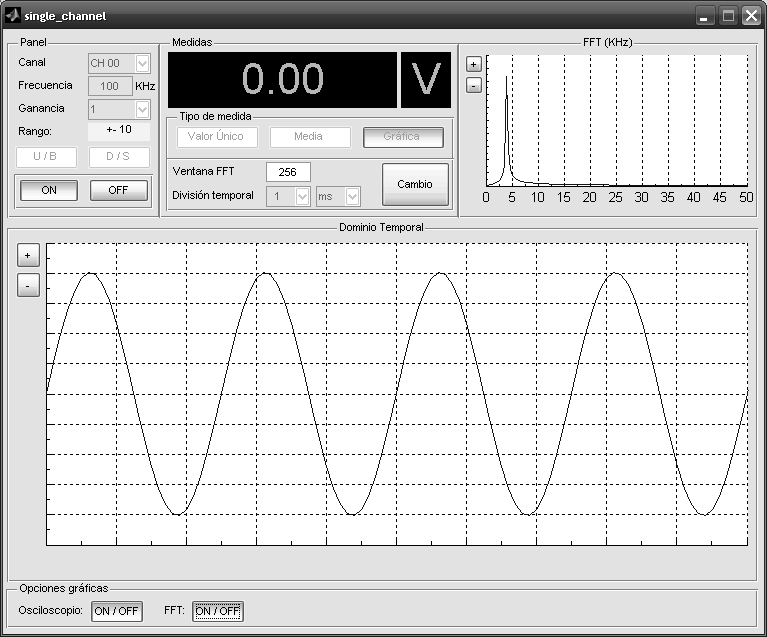
\includegraphics{gis-pfc-ch4-01.png}
    \end{center}
    \caption[Configuración por defecto]{Representación de los datos
    utilizando la configuración por defecto.}
    \label{fig:default}
\end{figure}

\begin{figure}[p]
    \begin{center}
	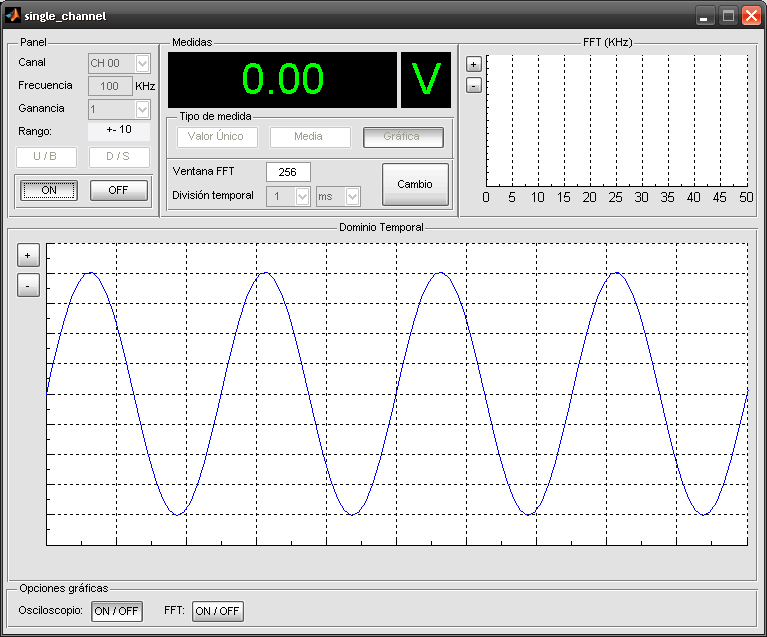
\includegraphics{gis-pfc-ch4-02.png}
    \end{center}
    \caption[Representación del espectro de la señal
    inhabilitada]{Representación del espectro de la señal inhabilitada.}
    \label{fig:specter-disabled}
\end{figure}

\begin{figure}[p]
    \begin{center}
	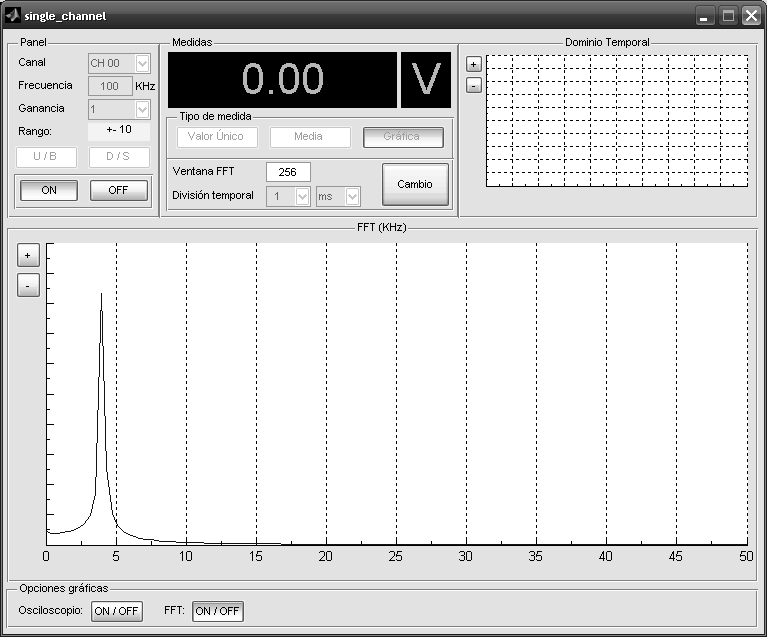
\includegraphics{gis-pfc-ch4-03.png}
    \end{center}
    \caption[Representación de la señal deshabilitada]{Representación de la
    señal deshabilitada.}
    \label{fig:signal-disabled}
\end{figure}

\begin{figure}[p]
    \begin{center}
	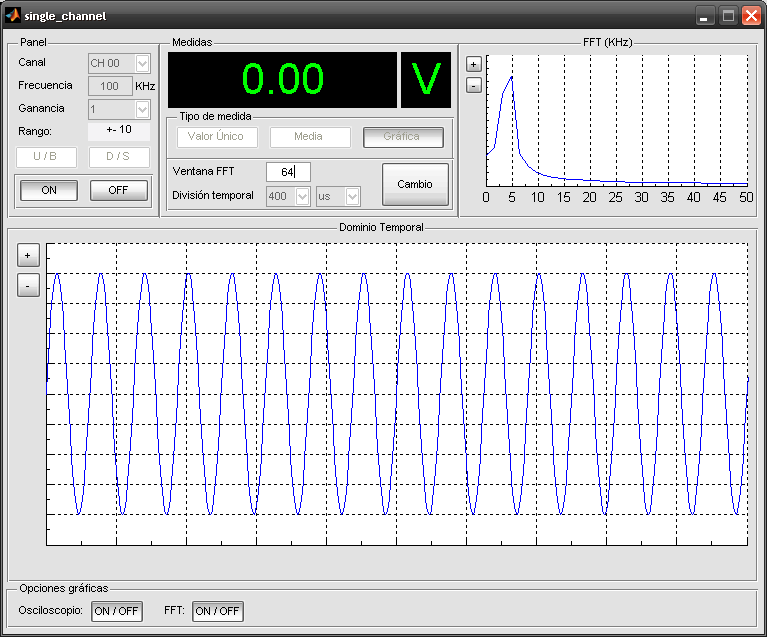
\includegraphics{gis-pfc-ch4-04.png}
    \end{center}
    \caption[Selección de otra escala temporal]{Se representa la señal
    empleando una escala temporal distinta (duración del fragmento
    representado por defecto de 1 ms, duración seleccionada $0.4$ ms.}
    \label{fig:scaled}
\end{figure}

\begin{figure}[p]
    \begin{center}
	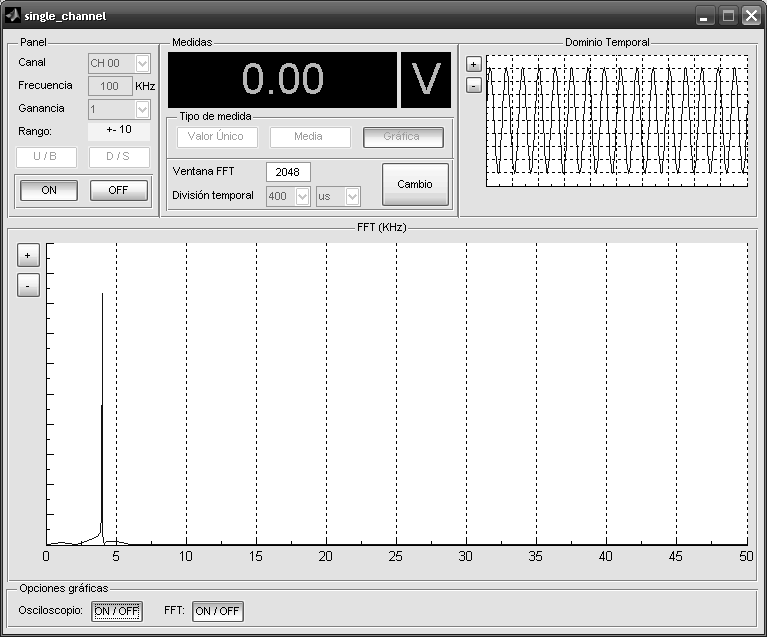
\includegraphics{gis-pfc-ch4-05.png}
    \end{center}
    \caption[Selección de un número de puntos distinto para la realización
    de la \sig{fft}]{Selección de un número de puntos distinto para la
    realización de la \sig{fft}.}
    \label{fig:point-number}
\end{figure}


\section{Conclusiones y futuras líneas de trabajo}

Los resultados observados en apartados anteriores certifican que se ha
logrado desarrollar satisfactoriamente un sistema de medida con las
siguientes prestaciones:

\begin{itemize}
    \item Seguimiento del valor numérico instantáneo de la señal.
    \item Cálculo de la media aritmética cada 250 ms.
    \item Representación gráfica continua o disparada de la señal.
    \item Simultáneamente, representación gráfica del espectro en
	frecuencias de la señal (\sig{fft}).
\end{itemize}

Este sistema de medida presenta, no obstante, las siguientes limitaciones
conocidas:

\begin{itemize}
    \item Inherentes a los componentes del sistema:
	\begin{itemize}
	    \item La frecuencia de las señales que pueden representarse
		está limitada a 25 kHz.
	    \item El modo continuo de representación (adecuado para
		representar señales de frecuencia inferior a 5 Hz) no
		funciona apropiadamente en equipos sin aceleración gráfica.
	    \item La caja de conexiones induce la aparición de señal en
		puertos situados en la misma fila que el puerto utilizado.
	\end{itemize}
    \item Inherentes al código fuente de la aplicación:
	\begin{itemize}
	    \item La aplicación carece de las funciones de autoajuste y
		disparo automático.
	    \item La aplicación no muestra medidas automáticas de los
		parámetros de la señal.
	    \item Los controles para ajustar la escala temporal, el número
		de puntos para el cálculo de la \sig{fft} y la escala de
		amplitud pueden mejorarse.
	    \item La aplicación carece de cursores para evaluar
		gráficamente los parámetros de la señal.
	    \item No es posible seleccionar la frecuencia con la que se
		calcula la media aritmética de los datos obtenidos.
	\end{itemize}
\end{itemize}

En el futuro sería recomendable actualizar el equipo que conforma el
sistema de medida, especialmente la tarjeta de adquisición, para obtener
unas mejores prestaciones. Además es posible mejorar la aplicación
incorporando nuevas funcionalidades a las que ya están disponibles.


\subsection{Subsistema para la interacción con el medio
físico}\label{subsec:transducerconclusions}

El sistema de medida digital obtenido como resultado del proceso de diseño
y desarrollo que ocupa esta primera parte del proyecto se pone a prueba al
realizar una serie de ensayos ultrasónicos preliminares que pretenden
evaluar la capacidad del sistema para encontrar resultados válidos. Estos
ensayos se realizan en el laboratorio a partir de muestras extraídas de
palmeras muertas (listones y tablones de madera de palmera). Los resultados
arrojados por las pruebas demuestran que la onda ultrasónica que emiten el
actuador no es capaz de atravesar los tablones de 20 cm de espesor
utilizados en el experimento. Se llega por tanto a la conclusión de que los
transductores de gama baja utilizados para la confección del subsistema
para la interacción con el medio físico, a pesar de ser apropiados para
aplicaciones como un detector de proximidad, no reúnen las condiciones
necesarias para ser utilizados en un \sig{endus}.

Además, un estudio posterior realizado durante el desarrollo de este
documento ha revelado el importante papel que adquieren los circuitos de
acondicionamiento en los ensayos no destructivos por ultrasonidos. Por todo
ello se recomienda la renovación de los transductores, por unos de mayor
potencia, y una vez renovados éstos, la realización de los circuitos
acondicionadores apropiados para extraer el máximo partido a los nuevos
transductores.

\part[\textsc{endus} en madera de palmera] %
{Ensayos no destructivos en madera de palmera}
\pagestyle{number}						% fancyhdr
\chapter*{Introducción}

\section*{Organización de la segunda parte}

La segunda parte está dividida en dos capítulos: el quinto capítulo, que
trata los fundamentos teóricos de los \sig{endus}; y el sexto, en el que se
exponen los resultados extraídos de los ensayos, las conclusiones a las que
se ha llegado, así como las líneas de trabajo que se preven para futuros
proyectos relacionados con la materia.

\begin{description}
    \item[Quinto capítulo] En el primer capítulo de esta parte se describe,
	de forma superficial, los distintos elementos que intervienen en un
	\sig{endus} desde un punto de vista teórico. De las distintas
	técnicas existentes para combatir el ruido estructural se dan
	detalles sobre las de procesado por partición del espectro que son
	las que se propone utilizar en futuros proyectos.
    \item[Sexto capítulo] El último capítulo recoge los resultados
	extraídos de las pruebas en forma de grafos y tablas comentados.
	Después se dan las conclusiones a las que se ha llegado a partir de
	estos resultados y finalmente se realizan una serie de comentarios
	sobre nuevas líneas de investigación que pueden seguirse de este
	proyecto
\end{description}

\pagestyle{body}						% fancyhdr
\chapter{Teoría de los \textsc{endus}}\label{chap:endus}

Los ultrasonidos son ondas acústicas de naturaleza mecánica o elástica como
los sonidos. A diferencia de las ondas sónicas los ultrasonidos se
encuentran en una banda de frecuencia superior. Dicha banda parte de los 20
kHz y, carente de un límite físico, llega hoy hasta los 1000 MHz debido a
limitaciones tecnológicas. Las frecuencias empleadas en los ensayos no
destructivos se encuentran entre los 20 kHz y los 25 MHz. Cabe remarcar que
las propiedades de las ondas acústicas se mantienen invariantes con la
frecuencia, y por tanto, son comunes dentro del espectro acústico.

Las ondas ultrasónicas son perturbaciones mecánicas que viajan a través de
un medio elástico, por tanto, la condición primordial para que las ondas
ultrasónicas se propaguen a través de un medio es que este contenga
fracciones de materia tales como átomos o moléculas susceptibles de vibrar.
El medio determina también que modos de propagación pueden adoptar las
ondas ultrasónicas que se propagan a su través. Frecuentemente se asocia un
nombre característico a las ondas ultrasónicas en función del modo en el
que se propagan por el medio. A continuación se exponen los modos de
propagación de mayor relevancia.

\begin{itemize}
	\item Las \emph{ondas longitudinales}, también llamadas \emph{ondas
		de presión o compresión}, son aquellas que oscilan en la
		dirección de propagación. Al contrario que el resto de
		modos de propagación que sólo se dan en sólidos, el modo
		longitudinal puede estar presente también en líquidos y
		gases.
	\item En las \emph{ondas transversales o de cizalladura} las
		oscilaciones se producen en la dirección perpendicular a la
		dirección de propagación.
	\item Las \emph{ondas de superficie} se propagan únicamente a
		través de sólidos semi"=infinitos cuya superficie sea plana
		o curva y siempre siguiendo las irregularidades del
		contorno del mismo.
	\item Las \emph{ondas de Lamb o de chapa} son propias de medios
		sólidos en los que el espesor es del mismo orden que la
		longitud de onda, provocan la vibración de todo el
		material.
\end{itemize}

La energía acústica que se propaga por un medio se manifiesta en forma de
presión acústica, esta a su vez define el campo acústico. La presión
acústica se define como:

\begin{equation}
	p = Z\cdot v
	\label{eq:acuospressure}
\end{equation}

Ecuación en la que $v$ representa la velocidad de vibración y $Z$ la
impedancia acústica. La impedancia acústica es una medida de la resistencia
con que se oponen los elementos de masa de un medio a la vibración
provocada por las ondas acústicas, en ningún caso da una relación de la
resistencia con la que el medio se opone a la propagación de la onda
acústica. Es una constante del medio que aumenta con la cohesión de sus
moléculas, y puede expresarse en función de la densidad $\rho_0$ y de la
velocidad de propagación de las ondas ultrasónicas en dicho medio $c$.

\begin{equation}
	Z = \rho_0\cdot c
	\label{eq:Zacoustic}
\end{equation}


\section[Campo acústico generado por un transductor]{Campo acústico
generado por un transductor de ultrasonidos}\label{sec:field}

La excitación eléctrica de un transductor produce una onda de presión que
se propaga en el medio siguiendo las leyes físicas de la propagación de
ondas y, en particular, los principios de superposición de
Huygens\footnote{El tratamiento que se da en esta sección a los
transductores de ultrasonidos es similar al que la teoría de antenas da a
las antenas de apertura conocidas como bocinas. Para un mayor detalle
consultar el texto de Stutzman y Thiele \citep{stutzman1997atd}.}. Se
denomina campo acústico a la distribución temporal y espacial de la presión
acústica a la que se someten las partículas materiales del medio en el que
se propagan las ondas acústicas. Las características del campo acústico
dependen principalmente de aspectos geométricos del transductor.

La región del campo acústico más próxima al transductor se conoce como
campo próximo o cercano. También recibe el nombre de campo de interferencia
debido a que en esa región el campo está constituido por máximos y mínimos
que surgen como resultado de las interferencias que se producen entre las
señales originadas en los distintos puntos del transductor. El máximo
principal del campo acústico delimita la región de campo próximo. La
longitud de esta región puede calcularse a partir del diámetro del
transductor $D$, o en su defecto a partir de la dimensión principal de
este.

\begin{equation}
	L_0 = \frac{D^2}{4\lambda}
	\label{eq:nearfield}
\end{equation}

Más allá del campo cercano encontramos el campo lejano. En el campo lejano
el frente de ondas de la radiación acústica empieza a divergir. Se llama
ángulo de divergencia del haz a la razón con la que el haz se expande y se
emplea el símbolo $\gamma_0$ para representarla. Puede calcularse
$\gamma_0$ a partir de la siguiente expresión.

\begin{equation}
	\sin{\gamma_0} = 1.2\cdot\frac{\lambda}{D}
	\label{eq:Adivergence}
\end{equation}

\begin{figure}
	\begin{center}
		\includegraphics{gis-pfc-ch5-01.pdf}
	\end{center}
	\caption[Campo acústico generado por un transductor
	cilíndrico]{Diagrama simplificado que muestra el campo acústico
	generado por un transductor cilíndrico.}
	\label{fig:transceiver}
\end{figure}

En la \vref{fig:transceiver} el lector puede observar una representación
del campo acústico generado por un transductor de ultrasonidos cilíndrico.
Puede observarse la forma geométrica del campo próximo tal y como se ha
considerado en este documento: un cilindro de radio igual al del
transductor y altura $L_0$. En el interior del cilindro el campo acústico
permanece constante y en el exterior el campo es nulo. A continuación se
ilustra como el frente de ondas diverge en el campo lejano. La figura
empleada para representar el campo lejano es un tronco de cono en cuyo
interior el campo acústico iría incrementando de la superficie al eje.

Para finalizar este punto cabe mencionar que el transductor es responsable
de que una determinada región de los materiales inspeccionados no pueda ser
caracterizada mediante el uso de ultrasonidos. La razón es que tras emitir
un pulso acústico un transductor no cesa inmediatamente de vibrar, si no
que lo sigue haciendo durante cierto tiempo a su frecuencia natural de
oscilación con un factor de amortiguamiento que depende de factores
constructivos. A la región del material que no puede ser inspeccionada se
la conoce como zona muerta o zona ciega. La zona ciega de un material
empieza en la superficie que está en contacto con el transductor y su
profundidad depende de la duración de los pulsos acústicos.


\section[Técnicas empleadas en las inspecciones ultrasónicas]{Técnicas
empleadas en las inspecciones ultrasónicas, en
\protect{\textbf{\textsc{endus}}}}\label{sec:technics}

Atendiendo a la situación del receptor en los ensayos no destructivos
mediante ultrasonidos se distinguen dos técnicas: la técnica de pulso"=eco
y la técnica de transmisión. En la técnica de pulso"=eco el receptor suele
encontrarse cercano al emisor, de hecho es frecuente que un mismo
transductor haga las veces de emisor y receptor. Por el contrario en la
técnica de transmisión el receptor se coloca alineado en el eje del emisor
pero en el extremo opuesto del material inspeccionado.

\begin{figure}
    \begin{center}
	\subfloat[Inspección ultrasónica por transmisión]
	    [Inspección ultrasónica por transmisión.]{
	    \includegraphics{gis-pfc-ch5-02.pdf}}
	    \vspace*{.1\textheight}
	\subfloat[Inspección ultrasónica por pulso"=eco]
	    [Inspección ultrasónica por pulso"=eco.]{
	    \includegraphics{gis-pfc-ch5-03.pdf}}
    \end{center}
    \caption[Técnicas empleadas en \sig{endus}]{Diferencias en cuanto al
    número y posición de los transductores según la técnica empleada en una
    evaluación mediante ultrasonidos.}
    \label{fig:technics}
\end{figure}

Al propagarse un pulso acústico por el medio, parte de éste se refleja al
encontrarse con discontinuidades en la impedancia acústica, otra parte
seguirá avanzando hasta atravesar el material o verse completamente
atenuada. La señal que capta el receptor depende de su ubicación. De este
modo la señal recibida cuando la técnica empleada es la de pulso"=eco es la
suma de los pulsos reflejados o ecos. Si la técnica utilizada es la técnica
de transmisión se percibe el pulso original, modificado por haber
atravesado el medio. La información que contiene la señal recibida es, por
tanto, diferente.

La técnica de pulso"=eco se centra en el estudio de la amplitud, forma y
posición temporal de los ecos. La técnica de transmisión por su parte
observa posibles cambios de velocidad en el pulso acústico y mide la
atenuación que éste experimenta al pasar a través del medio. La información
que proporciona el estudio de los ecos es más rica pero también más
compleja. Por consiguiente la elección de una u otra técnica está
supeditada no sólo a las posibilidades de inspección que ofrece el medio,
si no también al tipo de información que se pretende obtener con el ensayo.


\section{Parámetros de calidad en una inspección}\label{sec:quality}

Los parámetros de calidad proporcionan una medida cualitativa de la bondad
de un ensayo. Los más empleados son resolución, linealidad y relación señal
a ruido.

En ensayos no destructivos la resolución es la distancia mínima (o una
medida en relación con ésta) a la que deben encontrarse dos singularidades
cercanas para que ambas sean detectadas distinguiéndose una de la otra. Se
hace distinción entre resolución axial y resolución lateral. La primera
alude a la distancia que debe haber entre dos singularidades alineadas en
la dirección longitudinal de propagación de las ondas acústicas, la segunda
a la que debe haber entre singularidades que se encuentren dispuestas en
una línea normal a esa dirección.

Atendiendo a la definición de resolución que se ha proporcionado, se
considera que la resolución es mejor si la distancia mínima disminuye y
peor si ésta aumenta. Teniendo esto en cuenta, para mejorar la resolución
axial de un sistema es necesario emplear dispositivos de banda ancha y
emitir pulsos estrechos de alta frecuencia. La frecuencia de los pulsos
acústicos está limitada por el espesor del medio, a medida que aumenta la
frecuencia disminuye la profundidad de penetración del pulso, resulta pues
conveniente adoptar una solución de compromiso.

La resolución lateral depende también de la frecuencia del pulso, es mejor
a medida que aumenta la frecuencia puesto que disminuye la longitud de
onda. Además depende del diámetro de los transductores, es peor cuanto más
anchos son éstos. Y en la región de campo lejano, la resolución lateral
empeora a medida que aumenta la profundidad.

El comportamiento de la resolución lateral con respecto al diámetro del
transductor y la frecuencia del pulso acústico transmitido, descrito en el
párrafo anterior puede deducirse de las ecuaciones
\cref{eq:nearfield,eq:Adivergence}. Puede observarse que, a medida que
aumenta la frecuencia y disminuye la longitud de onda del pulso, aumenta la
longitud de la región de campo cercano. En dicha región el campo acústico
se encuentra contenido en un cilindro de radio el del transductor, como ya
se ha mencionado, y a partir de ahí empieza a divergir según una razón que
disminuye con la longitud de onda. Para una mejor resolución es pertinente
que la región activa del campo ultrasónico sea lo más estrecha posible, de
ese modo se evita en la medida de lo posible que dos anomalías cercanas
queden cubiertas por el haz en un mismo evento de la secuencia de barrido.
Por tanto, se confirman por medio de estas ecuaciones los beneficios en
términos de resolución que resultan del uso de transductores de diámetro
estrecho y de pulsos ultrasónicos de alta frecuencia.

La definición y comportamiento de linealidad y relación señal a ruido son
los habituales en términos de sistemas electrónicos, por eso se entiende
que el lector tiene una noción al respecto y no se dan más aclaraciones en
este apartado.


\section{El problema del ruido en las inspecciones}\label{sec:noise}

La principal limitación en las inspecciones ultrasónicas es el ruido. Los
ensayos de este tipo se ven afectados generalmente por varias fuentes de
ruido. Según su naturaleza estadística el ruido perjudica en mayor o menor
medida los resultados de un ensayo. Cuanto más se asemeje el ruido a la
señal desde el punto de vista estadístico más la perjudicará y más difícil
será contrarrestar su efecto. El \emph{ruido incoherente aleatorio} tiene,
como su propio nombre indica, un origen aleatorio, y en consecuencia no
está relacionado con la señal. Por el contrario, los mecanismos que
originan el \emph{ruido coherente} son con frecuencia los mismos que dan
lugar a la señal de interés, y de ahí que exista una fuerte relación entre
el carácter estadístico de ambas señales.

Entre los exponentes más comunes de ruido incoherente aleatorio encontramos
el \emph{ruido gaussiano} y el \emph{ruido impulsivo}. El primero es
inherente a los equipos electrónicos y su origen es térmico, el segundo
tiene origen en las interferencias electromagnéticas causadas por equipos
eléctricos situados en las proximidades del sistema empleado para el
ensayo. Este tipo de ruido puede ser combatido sin dificultad con técnicas
bien conocidas como son: el promediado temporal de señales, el filtrado
paso-banda, la autocorrelación o las técnicas de compresión de pulsos, en
el caso del ruido gaussiano; y algoritmos de filtrado no lineal, en el caso
del ruido impulsivo.

En ensayos no destructivos mediante ultrasonidos, la señal de interés y el
\emph{ruido estructural o de grano} tienen una misma procedencia. Ambas
señales surgen como consecuencia de interactuar un pulso acústico con los
distintos elementos de que se compone un material. En el caso de la primera
de las señales, el pulso se refleja en las posibles particularidades
presentes en el medio como grietas o hendiduras. En el caso del ruido, las
reflexiones se producen al encontrarse el pulso con las partículas
suspendidas en el medio y de las que éste se compone. Las diferencias entre
ambas señales radican en el tamaño y distribución de los elementos
reflectantes en el medio. Los reflectores que provocan el ruido son de
tamaño inferior a la longitud de onda de la señal propagada, y se
encuentran cercanos entre sí dispuestos de forma aleatoria por el medio.
Esto provoca que el carácter de la señal que aquí se ha bautizado como
ruido estructural sea, a efectos de una inspección ultrasónica, aleatorio e
impredecible. Si bien, la naturaleza de estas señales es similar y en
concreto lo es su naturaleza estadística. Por eso el ruido estructural es
considerado un ruido de tipo coherente y resulta complicado neutralizar su
efecto en los resultados del ensayo. Aún más, este ruido es el principal
factor limitante en ensayos de este tipo, enmascarando detalles en la señal
de interés que aportan información sobre posición, tamaño y forma de las
singularidades que son objeto de estudio. En contraposición a este hecho,
es posible emplear esta señal, que aquí es indeseada y considerada ruido,
en otro tipo de trabajos con el objetivo de caracterizar las propiedades
acústicas de un material.


\section{Fundamentos físicos del ruido estructural}

El ruido estructural es una consecuencia directa de la dispersión. Cuando
un frente de ondas incide sobre una partícula de tamaño comparable a su
longitud de onda, la energía que transporta se dispersa por la acción de
esa partícula. Dicha partícula actúa como un reflector esférico y selectivo
en frecuencia ---afectando más a las altas frecuencias\footnote{Según la
relación $c = \lambda\cdot f$, si se mantiene $c$, a medida que aumenta $f$
disminuye la longitud de onda y, por tanto, el tamaño de la partícula con
respecto a la longitud de onda aumenta.}--- que refleja la señal en todas
direcciones. De este modo, aquellos materiales que contienen un número
considerable de partículas susceptibles de interferir del modo descrito en
la propagación de un determinado frente de ondas, son considerados
materiales dispersivos.

En el caso de un frente de ondas acústicas que incide sobre un determinado
material dispersivo, la energía que tras el proceso de reflexión se propaga
en sentido contrario al de propagación del frente de ondas se conoce como
\emph{back-scattering}. Por su parte, la energía perturbada por la acción
del reflector que continúa propagándose en el mismo sentido suele
denominarse \emph{forward-scattering}. En los \sig{endus} dependiendo de la
técnica empleada es uno u otro tipo de dispersión el que causa un mayor
deterioro de los resultados: si la técnica empleada es de pulso"=eco, el
\emph{back-scattering} será el más perjudicial; si, por el contrario, se
está empleando la técnica de transmisión, será el \emph{forward-scattering}
el más nocivo para el proceso.

Para poder estudiar el efecto del ruido estructural en las inspecciones
ultrasónicas de forma adecuada es necesario caracterizar el proceso de
emisión"=recepción que se da en un ensayo mediante ultrasonidos desde el
punto de vista de la respuesta al impulso o régimen transitorio.


\subsection{Análisis del proceso de emisión-recepción}

Los diferentes elementos que intervienen en el proceso de
emisión"=recepción de que consta una inspección ultrasónica tienen un
comportamiento lineal, esto permite estudiar todo el conjunto como un
sistema lineal, y ello a su vez posibilita el uso de técnicas propias del
análisis de este tipo de sistemas.

Supóngase un transductor de perfil arbitrario, al excitarse con un pulso
eléctrico, $u(t)$, y dadas a sus propiedades electromecánicas, emite un
pulso acústico de velocidad $v(t)$ relacionado con la respuesta impulsiva
de emisión del transductor, $h_{te}(t)$.

\begin{equation}
	v(t) = h_{te}(t)\otimes u(t)
	\label{eq:emiter}
\end{equation}

La respuesta impulsiva electrodinámica en emisión, $h_{te}(t)$ depende del
circuito electrónico empleado para excitar el transductor y de los
parámetros de diseño de este último.

La presión en un punto situado en el eje $y$ y a una distancia $z$ del
transductor es el resultado de la suma coherente de las aportaciones de
cada uno de los puntos que forman la cara del transductor por la que emite
la onda acústica, considerándolos como emisores omnidireccionales y
esféricos. La presión en cada punto del espacio está relacionada con la
velocidad en la cara del pistón por medio de la siguiente expresión:

\begin{equation}
	p(z, t) = \rho\,\frac{\partial}{\partial t}\left\{v(t)\otimes
	h_{m}(z, t)\right\}
	\label{eq:diffracpressure}
\end{equation}

Siendo $\rho$ la densidad del medio por la que se propaga la onda acústica
y $h_{m}(z, t)$ la respuesta al impulso en el medio de propagación
considerando la difracción que se produce en dicho medio.

La propagación de una onda acústica se ve sometida a fenómenos de
difracción propios de la naturaleza ondulatoria de la radiación acústica y
fenómenos de atenuación a consecuencia de la interacción con el medio. De
cara al estudio de la propagación de la onda estos fenómenos pueden
tratarse por separado. Por un lado se considera el efecto de la difracción
sobre la onda en un medio homogéneo y sin pérdidas, y por otro la
atenuación que induce el medio. Esta aproximación mantiene su validez
siempre que el estudio afecte a una región del campo muy próxima al
transductor. Si se considera esta aproximación, y se tiene $h_d(z, t)$, la
respuesta al impulso en un medio homogéneo y sin pérdidas a la difracción,
y $a(z, t)$, la atenuación atribuida al medio; puede descomponerse la
respuesta al impulso en el medio de propagación a la difracción en esos dos
términos:

\begin{equation}
	h_m(z, t) = h_d(z, t)\otimes a(z, t)
	\label{eq:diffraction}
\end{equation}

La atenuación es selectiva en frecuencia y ello se asocia a los siguientes
aspectos derivados de la existencia de una macro y una micro"=estructura en
el material:

\begin{itemize}
	\item La absorción o transformación de la energía acústica que
		transporta la onda en calor.
	\item Y los efectos de dispersión de la energía.
\end{itemize}

La expresión que define la atenuación sufrida por la onda acústica toma la
siguiente forma a partir de $\alpha(\omega)$ o coeficiente de atenuación
característico del medio.

\begin{equation}
	A(z, \omega) = e^{\int^z_0 -\alpha(z, \omega)dz} 
	\label{eq:loss}
\end{equation}

Cuando la onda acústica incide sobre un reflector, las características de
éste determinan la relación entre la onda incidente y la reflejada. Esta
relación viene dada por la función de reflectividad, $h_r(t)$, que depende
de la frecuencia de la onda de presión. Si la reflexión que se produce al
llegar la onda hasta la partícula es especular, $h_r(t)$ coincide con una
delta de Dirac ponderada.

Como consecuencia de la reflexión, una señal distinta de la emitida por el
transductor en origen regresa a éste. Por tanto, se produce en la cara del
transductor que da al material una presión variable con el tiempo $p_R(z,
t)$, constituida por la suma de la presión que se produce en cada punto de
la mencionada superficie.

\begin{equation}
	p_R(z, t) = p(z, t)\otimes h_r(t)\otimes h_m(z, t)
	\label{eq:recpressure}
\end{equation}

Del mismo modo, parte de la señal reflejada avanza en el mismo sentido de
propagación que la onda incidente. Si no es dispersada completamente en el
medio avanza hasta atravesar el material por completo. En ese caso, si es
la técnica de transmisión la empleada, una presión semejante a $p_R(z, t)$
se produce en la cara del transductor que se encuentra al otro extremo del
material. La función de reflectividad no varía, tan sólo cambia la
distancia que debe atravesar el frente de ondas hasta alcanzar el
transductor y, por tanto, es diferente la contribución de la respuesta al
impulso en el medio a la difracción, $h_m(z^\prime, t)$ en el segundo
trayecto.

Finalmente, la presión $p_R$ se traduce en una señal eléctrica en bornes
del transductor. Esta señal está relacionada con la respuesta impulsiva del
transductor en recepción, $h_{tr}(t)$, que depende, al igual que
$h_{te}(t)$ del circuito acondicionador y del proceso de fabricación del
transductor.

\begin{equation}
	y(t) = h_{tr}(t)\otimes p_R(z, t)
	\label{eq:receiver}
\end{equation}

Por consiguiente el proceso de emisión"=recepción en el que se fundamentan
los \sig{endus} puede describirse mediante la respuesta impulsional en
cascada de todos los fenómenos descritos.

\begin{equation}\label{eq:emirec}
	\begin{split}
		y(t) = \rho_0\frac{\partial}{\partial t}\{u(t)& \otimes
		h_{te}(t)\otimes h_d(z, t)\otimes a(z, t)\otimes \\
		&\otimes h_r(t)\otimes h_d(z, t)\otimes a(z, t)\otimes
		h_{tr}(t)\}
	\end{split}
\end{equation}

La \vref{fig:emirecmodel} muestra un diagrama de bloques que representa el
proceso de emisión"=recepción y todos los fenómenos que en el intervienen
según el modelo empleado en este documento. La función de transferencia del
sistema puede obtenerse de modo sencillo aplicando el teorema de la
convolución.

\begin{figure}
	\begin{center}
		\includegraphics[scale=1, keepaspectratio=true]%
		{gis-pfc-ch5-04.pdf}
	\end{center}
	\caption[Diagrama que representa el proceso de
	emisión"=recepción]{Diagrama de bloques que representa el proceso
	de emisión"=recepción y todos los elementos que en el intervienen
	(considerando el modelo propuesto).}
	\label{fig:emirecmodel}
\end{figure}

\begin{equation}
	\begin{split}
		Y(\omega) = j\omega\rho_0& \cdot U(\omega)\cdot
		H_{te}(\omega)\cdot H^2_d(z, \omega)\cdot
		A^2(z, \omega)\cdot \\
		&\cdot H_r(\omega)\cdot H_{tr}(\omega)
	\end{split}
	\label{eq:transference}
\end{equation}

Aprovechando la linealidad del sistema se agrupan los términos de la
función de transferencia en \eqref{eq:groupedtransference}, para que el
resultado quede en función de la respuesta electromecánica del transductor,
$X(\omega)$, y de la respuesta espacial al impulso, $H(z, \omega)$.

\begin{equation}
	Y(\omega) = X(\omega)\cdot H(z, \omega)\cdot A^2(z, \omega)
	\label{eq:groupedtransference}
\end{equation}

\begin{equation}
	X(\omega) = j\omega\rho_0\cdot U(\omega)\cdot H_{te}(\omega)\cdot
	H_{tr}(\omega)
	\label{eq:transducer}
\end{equation}

Siendo esta última, la respuesta espacial al impulso, función de la
posición del reflector y de su forma, o lo que es lo mismo, de las
funciones de reflectividad y difracción.

\begin{equation}
	H(z, \omega) = H^2_d(z, \omega)\cdot H_r(\omega)
	\label{eq:spacialresponse}
\end{equation}

Al agrupar de este modo la función de transferencia se establece de forma
explícita la separación entre los procesos de difracción y atenuación.
Además es posible establecer nuevas separaciones: dejando por un lado los
efectos debidos a los transductores y electrónica de acondicionamiento,
$X(\omega)$; por otro la influencia del medio en la onda que se propaga, es
decir, la atenuación, $A(z, \omega)$; y, finalmente, por otro los efectos
de la propagación y la interacción con el reflector, $H(z, \omega)$.


\subsection{Atenuación en medios dispersivos}

La atenuación es el fenómeno en el que se manifiesta la influencia del
medio en la propagación de una onda. Suponiendo un medio en el que la
atenuación depende únicamente de la frecuencia de la onda acústica, puede
calcularse la atenuación sufrida por dicha onda tras haberse propagado una
distancia $z$ a lo largo del medio, como:

\begin{equation}
	A(z, \omega) = e^{-\alpha(\omega)\cdot z}
	\label{eq:independentloss}
\end{equation}

Donde, como se anticipó en \eqref{eq:loss}, $\alpha(\omega)$ es el
coeficiente de atenuación. Cuando el material por el que se propaga la onda
es no homogéneo, la atenuación se debe a dos fenómenos:

\begin{description}
	\item[Absorción] Fenómeno que también aparece en medios homogéneos
		y por el cual la energía que transporta la onda se
		transforma en otro tipo de energía, por lo general en
		calor.
	\item[Dispersión] En este estudio se entiende dispersión como la
		distorsión que ejerce sobre el frente de ondas el grano
		suspendido en el medio. La acción del borde del grano, así
		como los saltos de índice de refracción que provoca la
		presencia de ese grano en el medio, contribuyen a la
		aparición de este fenómeno.
\end{description}

En el coeficiente de atenuación global vienen reflejadas las acciones que
sobre la señal ejercen ambos fenómenos. Siendo $\alpha_s(\omega)$ la
contribución de la dispersión y $\alpha_a(\omega)$ la contribución de la
absorción.

\begin{equation}
	\alpha(\omega) = \alpha_a(\omega) + \alpha_s(\omega)
	\label{eq:losscoefficient}
\end{equation}

El coeficiente de absorción depende del cuadrado de la frecuencia a la que
oscila el frente de ondas, $\alpha_a(\omega) = a_1\omega^2$. Siendo $a_1$
la constante de absorción del material. Por su parte, $\alpha_s(\omega)$
depende del tamaño, forma, orientación y distribución de los granos en el
medio, aunque también de la frecuencia como se muestra a continuación.


\subsection[Coeficiente de dispersión en medios dispersivos]{Estimación del
coeficiente de dispersión para un material dispersivo de naturaleza
granulosa}

El coeficiente de dispersión de un material no homogéneo de naturaleza
granulosa puede estimarse de forma teórica asumiendo que los granos en el
medio forman una matriz tridimensional de pequeños reflectores o granos
esféricos, tal y como se muestra en la \vref{fig:matrix}. Asumiendo este
modelo, puede obtenerse la respuesta global del medio obteniendo la
respuesta de un reflector e integrando a todo el volumen el resultado
obtenido para un solo grano.

\begin{figure}
	\begin{center}
		\includegraphics[scale=1, keepaspectratio=true]%
		{gis-pfc-ch5-05.pdf}
	\end{center}
	\caption[Modelo de pequeños receptores] {Modelo de pequeños
	receptores para la estimación del coeficiente de dispersión.}
	\label{fig:matrix}
\end{figure}

La \vref{eq:disperser} es una aproximación de la respuesta espacial al
impulso de un solo dispersor cuando sobre el incide un frente de ondas
ultrasónicas longitudinales plano. En esta ecuación se han empleado: $k$,
constante que depende de la geometría del reflector; la frecuencia angular
a la que oscila el frente de ondas, $\omega$; $c_l$, o velocidad a la que
se propaga el frente de ondas; $V$ volumen del dispersor; y $z$ distancia
entre éste y el transductor.

\begin{equation}
	H_s(z, \omega) = k\,\frac{V\omega^2}{zc^2_l}\,e^{-j2\omega z/c}
	\label{eq:disperser}
\end{equation}

De $H_s(z, \omega)$ se deduce que la onda reflejada es dependiente de la
frecuencia angular de oscilación. De hecho, se manifiestan las propiedades
de filtro paso bajo que muestra la partícula. Si el reflector es de tamaño
muy superior a la longitud de onda de la radiación acústica, la dependencia
de $H_s(z, \omega)$ con $\omega$ es en la práctica despreciable, y sólo
dependería de la geometría del reflector.

Si el conjunto de dispersores suspendidos en el medio es homogéneo, y todos
ellos están equiespaciados y presentan isotropía, es posible suponer que el
frente de ondas se encuentra de forma sucesiva y periódica con planos de
reflectores. Si se supone además que la contribución de la dispersión
múltiple es despreciable frente a la contribución de las reflexiones
primarias, el frente de ondas que se propaga tras el primer plano de
partículas es la suma vectorial de la onda no dispersada y de una pequeña
fracción de la onda que tras interactuar con dichas partículas sigue
propagándose en la misma dirección en la que se propaga el frente de ondas.
Si se tiene en cuenta el comportamiento de un plano de reflectores,
semejante a un filtro paso bajo, el resultado de la dispersión es \emph{un
frente de ondas que con respecto al original tiene atenuadas las altas
frecuencias}. Por tanto, puede manifestarse un equivalente, \emph{un
material dispersivo se comporta como un filtro paso bajo cuya
característica de atenuación depende de la profundidad que haya alcanzado
la onda en su propagación}.

Puede escribirse una expresión de la atenuación causada por la dispersión
si se considera ésta en función de la energía neta que aporta al frente de
ondas cada uno de los planos reflectores. Esta expresión queda en función
del diámetro del grano $D$, y de $s_1$, una constante de dispersión que
depende del material.

\begin{equation}
	A_s(z, \omega) = e^{-s_1D^3\omega^4z}
	\label{eq:dispersionloss}
\end{equation}

Mediante esta expresión y la \cref{eq:independentloss}, aplicando después
la \cref{eq:losscoefficient}, es posible calcular el coeficiente de
atenuación debido a la dispersión, $\alpha_s$, en la región de Rayleigh, en
la que $D\ll\lambda$. Empleando deducciones semejantes puede obtenerse el
coeficiente de atenuación en distintas situaciones de tamaño de grano y
longitud de onda.

{\setlength{\extrarowheight}{0.5ex}
\begin{equation}
	\alpha_s(\omega) = \left\{
	\begin{array}{c@{\qquad\text{---}\qquad}c@{\quad}c}
		s_1D^3\omega^4 & D\ll\lambda %
		& \text{(Región de Rayleigh)} \\
		s_2D\omega & D\simeq\lambda %
		& \text{(Región estocástica)} \\
		s_3/D & D>\lambda & \text{(Región de difusión)}
	\end{array}
	\right.
	\label{eq:dispersionlossreg}
\end{equation}}

\begin{figure}
	\begin{center}
		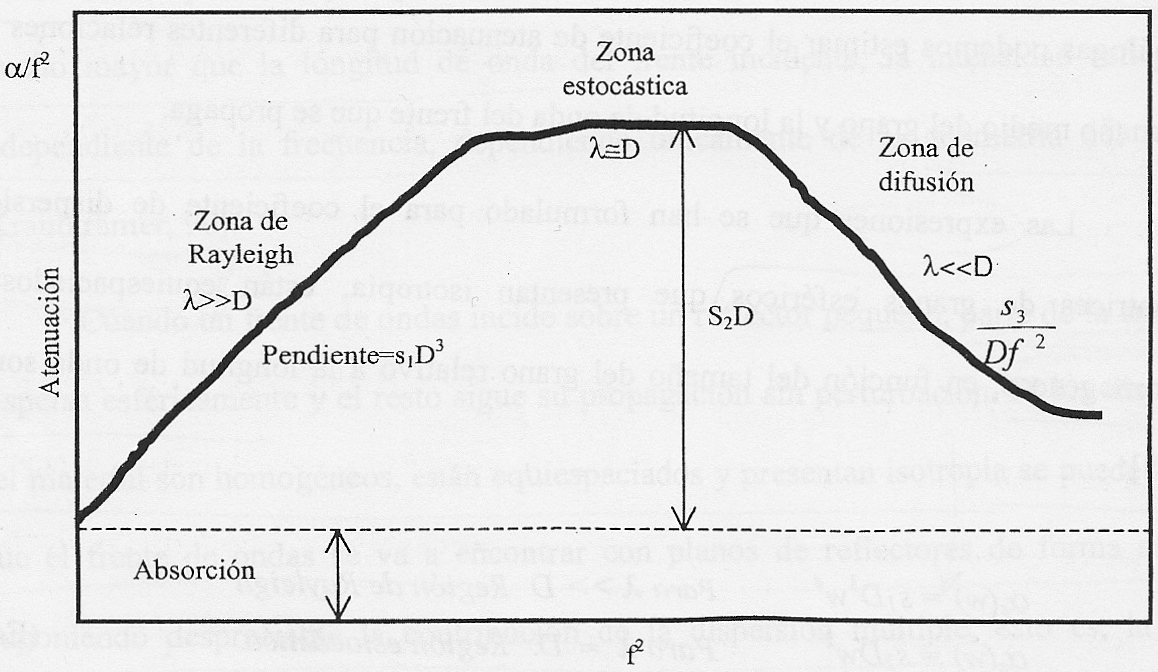
\includegraphics{gis-pfc-ch5-06.jpg}
	\end{center}
	\caption[Comportamiento del coeficiente de
	atenuación]{Representación del coeficiente de atenuación que
	muestra su comportamiento en las distintas regiones del material
	(figura extraída de \citealp{garcia2000mrsr}).}
	\label{fig:losscoefficient}
\end{figure}

Para finalizar este apartado, en la \vref{fig:losscoefficient} se muestra
una representación del coeficiente de atenuación, en concreto del cociente
$\alpha/f^2$, con respecto al cuadrado de la frecuencia. En la gráfica es
posible apreciar el comportamiento del coeficiente de dispersión en cada
una de las regiones descritas, y como el término que introduce la absorción
es de valor constante con la frecuencia. La región de difusión muestra una
atenuación abrupta que responde a una exponencial decreciente descrita por
la expresión $s_3/(Df^2)$.


\subsection[Limitaciones impuestas por la dispersión]{Limitaciones
impuestas por la dispersión en los ensayos ultrasónicos}

La dispersión, que contribuye de dos modos distintos a perjudicar el
proceso de inspección ultrasónica, por un lado atenuando la señal acústica,
por otro lado causando el ruido de grano, es el principal factor limitante
en los ensayos no destructivos. Es habitual que la dispersión limite la
profundidad de una inspección a la región de Rayleigh.

Cualquier material posee granos de diferentes tamaños y, por tanto, un
frente de ondas acústicas que atraviesa un material se ve afectado por la
dispersión como si se encontrase en las tres regiones de dispersión
descritas. No obstante, es el grano de mayor tamaño el que en la práctica
determina el comportamiento del material en términos de dispersión.

La dispersión, debido a que es la causante del ruido estructural, no puede
contrarrestarse aumentando la potencia de la onda ultrasónica en emisión.
La solución primera para evitar la dispersión pasa por disminuir la
frecuencia de la onda, pero esto desemboca también en una pérdida de
resolución. La mejor alternativa consiste en emplear técnicas de
procesamiento de señal que reduzcan la energía del ruido estructural en
recepción.


\section[Algoritmos para la reducción del ruido estructural]{Algoritmos
utilizados para la reducción del ruido estructural}

Dejando a un lado las técnicas empleadas en la eliminación de ruido
incoherente aleatorio, ineficaces por completo contra el ruido estructural,
existe un conjunto de métodos orientados a combatir este tipo de ruido.

Las técnicas empleadas con mayor frecuencia con el objeto de conseguir
mayor \sig{snr} en entornos en los que la presencia de ruido estructural es
notable son aquellas que aprovechan la diversidad de información hallada al
trabajar con señales incorreladas entre sí. Estas técnicas tratan de
obtener una señal con una mayor \sig{snr} a partir de la composición de
varias señales generadas mediante un mismo mecanismo pero de forma que la
medida de correlación entre cada una de ellas sea pobre. Los métodos
empleados más a menudo con tal propósito son:

\begin{itemize}
	\item Las técnicas que explotan la diversidad espacial, en las que
		básicamente se repite el mismo experimento variando cada
		vez la orientación de los transductores implicados en el
		mismo.
	\item Y las técnicas de diversidad frecuencial, manteniendo la
		posición de los transductores se repite el experimento
		utilizando señales situadas en una banda espectral
		diferente unas de otras.
\end{itemize}

Este tipo de técnicas consiguen mejorar de forma considerable la \sig{snr}
en inspecciones ultrasónicas, no obstante presentan una serie de
inconvenientes que las hacen inapropiadas en determinadas situaciones. Por
un lado, las técnicas de diversidad espacial se ven obstaculizadas con
frecuencia por las dimensiones y forma de las piezas evaluadas, siendo en
ocasiones imposible emplearlas. En cuanto a las técnicas de diversidad en
frecuencia, los transductores empleados en inspecciones ultrasónicas actúan
por lo común en una banda no lo bastante ancha como para poder dividirla en
un gran número de subbandas y así poder emitir suficientes señales
acústicas repartidas por el espectro de frecuencias. Para poder emplear una
técnica así serían necesarios varios transductores situados en la misma
posición que emitiesen simultáneamente en bandas de frecuencia distintas,
además la señal acústica emitida por cada transductor debería tener un
ancho de banda controlado.

La dificultad que conlleva implementar las técnicas anteriormente descritas
ha contribuido a la proliferación de técnicas que a partir de una única
traza sacan partido de las diferencias estadísticas que existen entre la
señal que procede de un defecto y el ruido estructural. Dentro de esta
categoría el algoritmo que ha alcanzado un éxito mayor y en consecuencia se
ha convertido en el paradigma de las técnicas de reducción de ruido
estructural se conoce como técnica de partición espectral o del inglés
\emph{Split Spectrum Processing} (\psig{ssp}) y fue en inicio propuesto por
Vernon Newhouse en 1982. El algoritmo está basado en la explotación de la
seudo"=diversidad frecuencial que existe entre las diferentes trazas de
banda estrecha que se obtienen al descomponer con un banco de filtros paso
banda la señal resultante tras un ensayo. No obstante los excelentes
resultados encontrados utilizando esta técnica, la gran sensibilidad que
muestra el algoritmo a la sintonía de los principales parámetros que
definen su comportamiento lo convierten en escasamente robusto. A
consecuencia de esto han aparecido numerosas publicaciones que se
circunscriben a proporcionar configuraciones del algoritmo que proporcionen
resultados óptimos, alternativamente aparecen también variaciones del
\sig{ssp} que persiguen mejorarlo. A pesar de su éxito, el \sig{ssp} no es
el único método empleado con el objetivo de sustraer el ruido de grano de
la señal de interés de un \sig{endus}. Otros trabajos incluyen, la
estimación de máxima verosimilitud, técnicas de filtrado paso"=banda que
eliminan la mitad superior del espectro de la señal, técnicas
tiempo"=frecuencia como son la transformada de Wigner"=Ville o las Wavelet,
técnicas que sacan partido de la información que aporta el retardo de
grupo, técnicas no lineales y, finalmente, técnicas de ruido residual.

A pesar del gran número de técnicas dedicadas a eliminar el ruido
estructural, son pocos los trabajos orientados a establecer una relación
entre ellas, a compararlas, a clasificarlas según su comportamiento en
distintos tipos de materiales o a justificar por qué el uso de una u otra
técnica.


\section{Técnicas de procesado por partición del espectro}

Bajo el término <<técnicas de procesado por partición del espectro>>, en
inglés \emph{Split Spectrum Processing Techniques}, o simplemente
\psig{ssp}, se reúnen una serie de algoritmos cuya aplicación es la
reducción del efecto del ruido estructural o de grano en los resultados de
un \sig{endus}. El principio en el que se fundamentan estas técnicas es
similar al que rige las técnicas de diversidad convencionales. A partir de
varias señales incorreladas entre sí se construye una señal cuya \sig{snr}
es considerablemente mejor que la \sig{snr} de cualquiera de las señales
primitivas por separado. Las técnicas de \sig{ssp}, a diferencia de las
técnicas basadas en la diversidad, consiguen sólo una seudo"=diversidad en
frecuencia a partir de una única traza de la señal que se obtiene tras un
\sig{endus}. Con frecuencia se obtienen buenos resultados empleando estas
técnicas lo que, sumado a la sencillez con la que puede implementarse un
experimento fundamentado en las mismas, recordando que no es requerida una
redundancia real basada en la utilización de varias señales, las ha
convertido en las técnicas más populares en el ámbito de los \sig{endus}. A
consecuencia de la reputación con la que se han visto revestidas
recientemente numerosas investigaciones se han llevado a cabo en las
décadas de los ochenta y los noventa, así como a principios de siglo, con
el fin de mejorar en la medida de lo posible los buenos resultados que ya
de por sí proporcionan las técnicas de \sig{ssp}.

El procedimiento (más detallado en el \cref{tab:sspfeatures}) que por lo
general sigue todo el conjunto de técnicas de \sig{ssp} consiste en aplicar
una transformación sobre la traza que comprende dos pasos:

\begin{itemize}
	\item El primero, dividir la traza en un número determinado de
		señales de banda estrecha, para lo que se emplea un banco
		de filtros.
	\item En segundo lugar se reconstruye la traza, o más bien una
		versión de ésta con una \sig{snr} mejorada, mediante un
		algoritmo de reconstrucción no lineal.
\end{itemize}

Las diferencias entre el carácter estadístico del ruido y de la señal
procedente del defecto hacen que el procedimiento anterior conduzca al
resultado deseado. Para concretar, la distribución de la energía del ruido
no es equitativa en frecuencia, de ahí que sea posible encontrar señales
incorreladas en ruido mediante la división espectral que realiza el banco
de filtros. Por otro lado, la linealidad que presenta la componente de la
señal ---o alteración de la misma según sea el caso--- originada en la
reflexión que se produce al encontrarse la onda acústica con el defecto
conlleva que la muestra que identifica la presencia del defecto se
encuentre en la misma posición en todas las trazas de banda estrecha. Los
métodos de \sig{ssp} aprovechan de manera implícita esta última
característica de la traza para magnificar la componente de la señal que
indica la presencia del defecto por lo que son catalogados en la
bibliografía como métodos que explotan la fase del defecto.


\begin{table}
	\centering
	\begin{tabulary}{.95\textwidth}{>{\((}c<{)\)}Lr@{\hspace{6pt}}L}
		\toprule
		\multicolumn{2}{c}{Parámetros} %
		& \multicolumn{2}{c}{Algoritmo} \\
		\cmidrule(r){1-2}\cmidrule(l){3-4}
		y & Señal a procesar & 1. & Generar del banco de filtros \\
		f_\text{min} %
		& Frecuencia inferior de corte del banco de filtros & 2. %
		& Calcular la \sig{fft} de $y$ \\
		f_\text{max} %
		& Frecuencia superior de corte del banco de filtros & 3. %
		& Procesar el resultado obtenido en (2) con el banco de %
		filtros \\
		\Delta f & Separación entre filtros & 4. %
		& Calcular la \sig{ifft} de las trazas de banda estrecha \\
		pb & Ancho de banda de los filtros & 5. %
		& Normalizar la amplitud de las trazas de banda estrecha \\
		h_f & Tipo de filtro empleado & 6. %
		& Construir una única traza a partir de las trazas de %
		banda estrecha normalizadas \\
		\bottomrule
	\end{tabulary}
	\caption[Particularidades propias de los algoritmos de
	\sig{ssp}]{Particularidades que en general se aplican a todos los
	algoritmos de \sig{ssp}.}
	\label{tab:sspfeatures}
\end{table}

\begin{figure}
	\begin{center}
		\includegraphics{gis-pfc-ch5-07.pdf}
	\end{center}
	\caption[Parámetros de configuración del banco de filtros]%
	{Representación esquemática en la que pueden observarse los
	parámetros empleados en la configuración del banco de filtros
	comparados con el espectro de la señal de audio.}
	\label{fig:filter}
\end{figure}

La eficacia de las técnicas de \sig{ssp} no está garantizada, depende en
gran parte de dos de los parámetros listados en el \cref{tab:sspfeatures}.
Por un lado está la configuración del banco de filtros, a destacar dos
aspectos: el tipo de filtro empleado y la zona del aspecto en la que se
aplica el método. Según afirma M.\,A. Izquierdo
\citep[en][]{garcia2000mrsr}, trabajos realizados a principios de los
noventa como los de P.\,Karpur apuntan a la existencia de una relación
entre el factor de forma de los filtros que se utilizan para realizar la
partición de espectro y la bondad de los resultados aportados por la
técnica de \sig{ssp}. Señala M.\,A. Izquierdo que, a pesar de que la
influencia que ejerce este parámetro en la calidad del ensayo haya mostrado
ser notable, estudios posteriores no han tenido en cuenta las conclusiones
alcanzadas por Karpur. La región del espectro que queda bajo el banco de
filtros puede configurarse ajustando las frecuencias de corte superior e
inferior del banco ---quedando indirectamente condicionados el ancho de
banda de los filtros y la separación entre los mismos---. Es importante
evitar que la banda de paso del banco coincida con alguna porción de la
señal en la que la información espectral que indica la presencia del
defecto quede enmascarada por el ruido de grano. Cuando así ocurre la
efectividad del método se reduce en gran medida.

El parámetro que resta por considerar no es otro que el algoritmo de
reconstrucción que permite recuperar la traza definitiva. Las técnicas de
\sig{ssp} se basan en la estabilidad de la fase, de ahí su precaria
robustez. El algoritmo de reconstrucción empleado es un factor determinante
del que depende en gran parte la robustez de la técnica. Por tanto, aplicar
un algoritmo de reconstrucción adecuado a las muestras es crucial para
obtener buenos resultados. Los algoritmos más empleados son el de mínimo
del ensamble y el del umbral de polaridad (\emph{Polarity Thresholding}) o
combinación de ambos, a continuación se citan otros.

Los trabajos mencionados en este apartado siguen todos una misma línea de
investigación, descubrir qué configuración del banco de filtros y qué
método de reconstrucción optimizan los resultados de aplicar las técnicas
de \sig{ssp} en un \sig{endus}. Se ha dicho que el término \sig{ssp} agrupa
a un conjunto de técnicas, lo que las diferencia precisamente es, o bien el
algoritmo de reconstrucción que emplean, o bien la forma en la que se
configura el banco de filtros, en ocasiones ambos. En cuanto a la
configuración del banco de filtros, algunos trabajos, en especial algunos
de Karpur, aportan avances significativos. El autor encuentra para el
algoritmo de mínimos, de forma analítica y apoyándose en un modelo
estacionario del ruido de grano, los parámetros que optimizan el
rendimiento de la técnica de \sig{ssp}. Los valores hallados son los
siguientes:

\begin{equation}
	\begin{split}
		N & = B\cdot T_y + 1 \\	
		b & = \Delta f = \frac{1}{T_y}
	\end{split}
\end{equation}

Donde $N$ representa el número óptimo de filtros, $B$ el ancho de banda del
transductor en el segmento de recepción, $T_y$ la duración de la señal
recibida, $b$ el ancho de banda de cada filtro, y $\Delta f$ la separación
entre filtros. Por otro lado Karpur afirma en otro de sus estudios, esta
vez apoyándose en la expresión para la atenuación en la región de Rayleigh,
que el banco de filtros debe aplicarse en las frecuencias más bajas del
espectro de la señal, ya que es en esa zona en la que se concentra la mayor
parte de la energía correspondiente a la radiación que tiene origen en el
defecto. Otros estudios utilizan la información relativa a la distribución
espectral de la \sig{snr}, obtenida mediante algoritmos como el del
histograma espectral o a partir de estadísticos del retardo de grupo como
p.e. la entropía móvil, para determinar cuál es la región del espectro de
la señal en la que es óptimo aplicar el filtrado.

En cuanto a los algoritmos de reconstrucción J.\,Saniie llega a la
conclusión, en su trabajo de 1991 en el que estudia los filtros de orden
aplicados como algoritmos de composición, de que los mejores resultados se
obtienen cuando la señal proviniente del defecto y el ruido estructural
están estadísticamente separados en un determinado cuantil. Dependiendo de
las distribuciones de probabilidad del ruido y del defecto, resulta
apropiado emplear algoritmos de mínimos, mediana o máximos del ensamble,
aunque por lo general el algoritmo de mínimos es el que mejores resultados
proporciona.

Por su parte M.\,G.\,Gustafsson propone una variante en el conjunto de las
técnicas de \sig{ssp} en la que, basándose en la teoría bayesiana de
detección y a partir de la información de la señal y el ruido coherente,
pueden encontrarse todos los parámetros necesarios para aplicar la técnica
de \sig{ssp}. El nombre que recibe usualmente esta variante es técnica de
\sig{ssp} con detección óptima.

\chapter{Caracterización de la madera de palmera por ultrasonidos}

El interés de la madera como material de construcción, o materia prima para
la fabricación de herramientas, instrumentos musicales, mobiliario o
carpintería naval ---por citar algunos ejemplos de la multitud de usos que
recibe la madera en la actualidad--- ha originado desde principios de siglo
un interés por el estudio de sus propiedades físicas. Recientemente los
ensayos no destructivos por ultrasonidos han tenido un papel importante en
el estudio de las características estructurales de la madera, especialmente
en la detección de discontinuidades como grietas, presencia de
acebolladuras o nudos. El interés por las propiedades estructurales de la
madera se justifica asimismo puesto que en muchas de sus aplicaciones de su
integridad depende la seguridad de sus usuarios, viendo como ejemplo más
claro de ello el uso de madera en la construcción.

Además, existe un interés patente por otras propiedades de la madera, como
sus propiedades mecánicas, al conocer las propiedades mecánicas de
distintos tipos de madera en distintas circunstancias es posible determinar
el mejor uso para cada tipo; o acústicas, la madera es útil en la creación
de cavidades resonantes o como aislante acústico pues muestra una alta
capacidad para atenuar el ruido. Los \sig{endus} han demostrado ser un
método efectivo para determinar las propiedades mecánicas y acústicas de la
madera.

Las palmeras, aunque también útiles para la construcción por sus
propiedades (al ser una madera blanda y ligera, la madera palmera se
utiliza sobre todo en la construcción de tejados y tejadillos), han pasado
a ser un importante elemento decorativo en los núcleos urbanos, e incluso
en ciertas localizaciones constituyen un elemento importante del patrimonio
cultural y medioambiental.

Como parte de la decoración urbana la palmera está sometida a la acción de
un medio hostil, en el que se dan grandes temperaturas y en el que sufre la
acción de agentes externos que en otros entornos no existen o muestran
menor actividad. Como género de plantas apreciado, existe un interés por
saber como afecta a la palmera su entorno, conocimiento que puede
alcanzarse contrastando las propiedades físicas de la madera de palmera
cuando está sujeta a la acción de distintos medios. Así mismo, la madera de
palmera defectuosa también puede ser causa de accidentes ---por ejemplo,
los jardineros debe subirse a las copas de las palmeras para su
mantenimiento, las palmeras que presentan deficiencias estructurales
constituyen un riesgo para su integridad física--- por lo que el
conocimiento de las características estructurales de un ejemplar,
especialmente de los ejemplares in vivo, adquiere vital importancia. Las
aplicaciones basadas en ultrasonidos parecen especialmente adecuadas al
tratar de deducir las propiedades físicas de palmeras vivas, pues cuentan
con la ventaja de no dañar el ejemplar.


\section{Objetivos del experimento}

La madera de palmera es desde el punto de vista de su estudio como medio de
propagación acústico dentro del conjunto de las distintas maderas cuanto
menos un medio peculiar podría decirse incluso, sin temor a equivocarse,
que es atípico. Ello se debe a las características propias del género; la
palmera, a pesar de ser una planta de tipo arbustivo crece ---la mayor
parte de las veces motivada por la acción del ser humano--- en forma
arborescente.

Ello se debe a las características propias del género, la palmera, a pesar
de su crecimiento en forma arborescente ---la mayor parte de las veces
motivado por la acción del ser humano--- es una planta de tipo arbustivo.
Es por ello que su tallo a pesar de ser leñoso muestra una composición
distinta a la madera de los árboles, no presenta madera secundaria pues sus
fibras no conservan procambium\footnote{Las fibras o haces vasculares de
las palmeras se denominan colaterales cerrados debido a esta propiedad. En
realidad, el tallo de una palmera es leñoso debido a que contiene
esclerénquima fibroso xilemático, un tejido celular elástico que le sirve
de sostén.} (tejido celular presente en los árboles responsable de su
crecimiento) con lo que carece de verdadero tronco.

De cara a su estudio, el tallo de una palmera presenta una estela (sección
transversal) en la que los haces vasculares formados en su mayor parte por
fibras xilemáticas y vasos liberianos (aquellos que transportan nutrientes
desde la parte autótrofa de la planta a sus partes basales subterráneas) no
se agrupan en ninguna estructura reconocible, si no que están dispersos
formando espacios entre sí rellenos con material blando y húmedo, y aire.
La gran proporción de humedad, el espacio vacío, y la distribución
heterogénea de las fibras dificulta enormemente la propagación de ondas de
media y alta frecuencia a través de un tallo de palmera, algo que no ocurre
en otros tipos de madera.

Actualmente existen muy pocas referencias bibliográficas que documenten que
tipo de información, parámetros o propiedades físicas pueden extraerse de
un ensayo por ultrasonidos en madera de palmera. En general, es muy difícil
encontrar información que relacione los parámetros físicos deducibles
mediante técnicas no destructivas basadas en ultrasonidos y las
características microestructurales inducidas por condiciones adversas en
madera de palmera. Menos aún si se trata de ensayos realizados con
transductores de impacto, pruebas realizadas con esta tecnología son muy
escasas.

Al disponer en el laboratorio de unos transductores de impacto,
recientemente obtenidos, se plantea como parte del proyecto fin de carrera
la realización de un estudio preliminar cuyos resultados puedan justificar
el interés en abordar un proyecto mucho más ambicioso en este campo. Cabe
remarcar aquí que como estudio preliminar este apartado del proyecto no
pretende aportar más que una serie de resultados que deberán valorarse
única y exclusivamente con el propósito aquí especificado.


\subsection{Elección de bajas frecuencias}

Es bien sabido (y se expone con detalle en el \vref{chap:endus} de esta
memoria) que las ondas ultrasónicas presentan un comportamiento variable
con respecto a la frecuencia. En este subapartado se justifica la elección
de las bajas frecuencias para el desarrollo de esta aplicación poniendo de
manifiesto cuales son las ventajas y desventajas que presentan en este tipo
de ensayos.


\subsubsection{Ventajas}

Como se observó en el capítulo anterior, uno de los principales
inconvenientes en los \sig{endus} es la aparición de ruido de grano. En
resumidas cuentas el ruido de grano es una señal originada en base al mismo
fenómeno que genera el eco que determina la presencia de defectos en el
material de estudio, la dispersión. Por ello es difícil diferenciar y
extraer el ruido de la señal recibida en un ensayo, lo que perjudica la
relación señal a ruido (por duplicado, ya que la dispersión forma parte de
la atenuación que afecta a la señal que se propaga) y dificulta la
obtención de resultados válidos. Las bajas frecuencias, mayores longitudes
de onda, no interactúan directamente con las partículas más pequeñas de un
medio por lo que presentan mayor inmunidad a este fenómeno y se ven
afectadas en menor medida por el ruido estructural.

Al verse menos afectadas por el efecto de la dispersión las ondas de baja
frecuencia se propagan satisfactoriamente a una mayor distancia permitiendo
el análisis de muestras a una mayor profundidad. Esta propiedad de las
ondas de baja frecuencia resulta útil cuando se desea explorar muestras de
un espesor notable o voluminosas como en este caso el tallo de un ejemplar
vivo de palmera. Además, en el caso de la madera de palmera, por su
composición, es preciso realizar los ensayos con ondas de baja frecuencia
ya que al beneficiarse de una mayor inmunidad frente a la dispersión son
las únicas capaces de propagarse a través de un medio como éste, realmente
hostil, hecho que por sí mismo justifica ampliamente su uso.


\subsubsection{Inconvenientes}

La principal desventaja de las bajas frecuencias frente a las medias y
altas frecuencias radica en que a medida que disminuye la frecuencia de la
onda empleada disminuye la bondad del ensayo, al menos en términos de
resolución. Esto puede no ser, sin embargo, demasiado importante
dependiendo de la aplicación, como es en el caso de este proyecto. Véase un
ejemplo explicativo: si lo que se desea es únicamente detectar un defecto y
no determinar su posición y forma exactas resulta más importante que la
onda ultrasónica alcance el sensor que que los resultados gocen de una
buena resolución.

Otro gran problema de las bajas frecuencias es que son más susceptibles de
viajar por la superficie de un material en lugar de atravesarlo.
Dependiendo del tipo de muestra y de sensor ésto puede resultar
inconveniente. En muestras en las que una de las dimensiones transversales
es muy pequeña la onda de superficie alcanza el sensor prácticamente al
mismo tiempo que la onda de propagación longitudinal, por lo que ambas
contribuciones se suman en el receptor actuando la onda superficial como
onda interferente. Sin embargo, en las muestras in vivo la distancia
recorrida por la onda superficial es prácticamente nula, tanto por el
diámetro de la muestra como por el relieve de su superficie, lo que
garantiza la viabilidad de los \sig{endus} en este sentido.


\section{Equipo utilizado}

Para la ejecución de las pruebas de campo destinadas a recoger las muestras
para la elaboración del estudio del material madera de palmera se ha
dispuesto de un conjunto de dispositivos y herramientas de diversa índole.
La \cref{fig:equipment} muestra parte del equipo utilizado. A continuación
se proporcionan unas breves notas sobre los elementos y configuraciones más
destacados.

\begin{figure}
    \begin{center}
	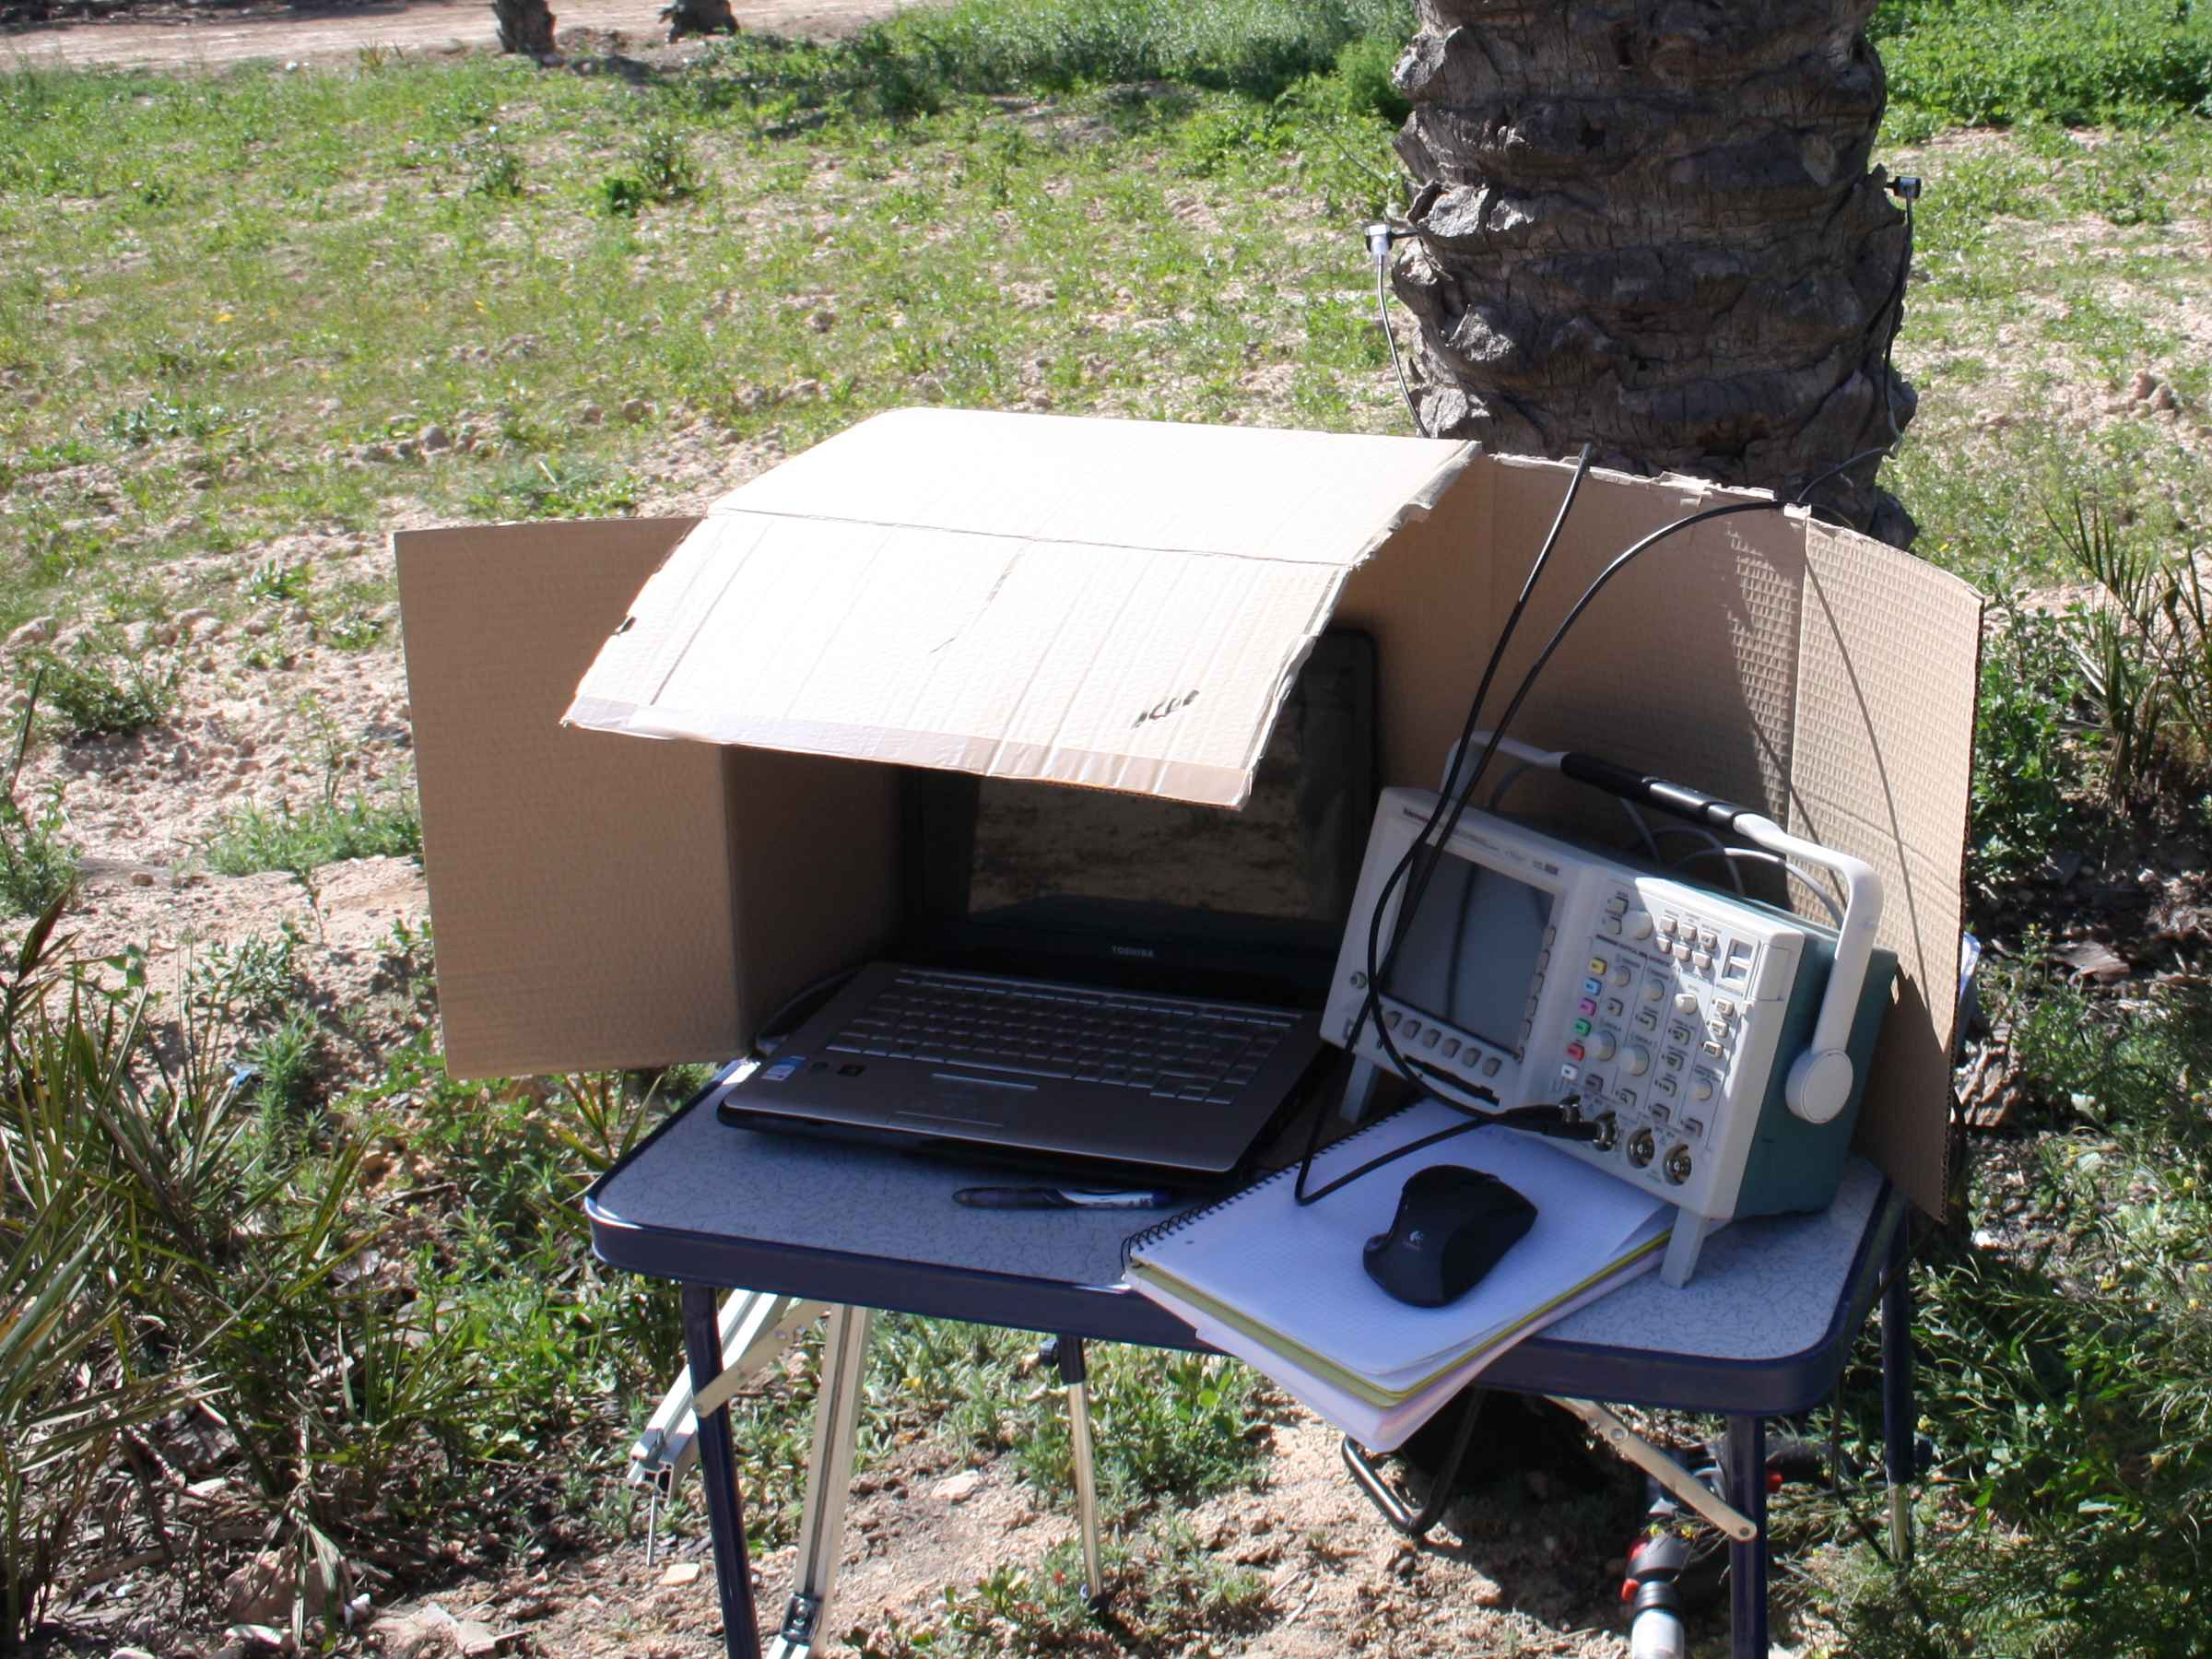
\includegraphics{gis-pfc-ch6-01.jpg}
    \end{center}
    \caption[Equipo utilizado durante los ensayos]{Equipo utilizado durante
    los ensayos realizados.}
    \label{fig:equipment}
\end{figure}


\subsection{Transductores de impacto}

Los transductores de impacto o sondas piezoeléctricas de impacto son
transductores específicos para aplicaciones que implican la realización de
ensayos no destructivos en ejemplares de árboles in vivo. En este caso
resultan útiles también para evaluar las propiedades de las palmeras puesto
que éstas crecen de forma arborescente. Están formados por un punzón que se
inserta levemente en el tallo del ejemplar sometido a estudio sin que ello
le cause ningún daño, quedando la sonda bien sujeta. El punzón canaliza
eficazmente la onda acústica transmitida al tronco del árbol, es capaz
igualmente de capturar la máxima energía que proviene del impulso
ultrasónico una vez éste se ha propagado por el medio. Los transductores de
impacto cuentan también con una cabeza metálica que recubre el propio
transductor, esta cabeza metálica está diseñada para poder amartillarse y
es capaz simultáneamente de resistir el impacto, protegiendo la parte
activa de la sonda, y de transmitir toda la fuerza del golpe al árbol por
medio de la onda acústica. Finalmente las sondas de impacto disponen de un
cable coaxial por medio del cual transmiten la señal eléctrica que generan
al sistema de medida; dicho cable está terminado en un conector de rosca
compatible con osciloscopios.

\begin{figure}
    \begin{center}
	\subfloat[Transductor utilizado como actuador][]{
	    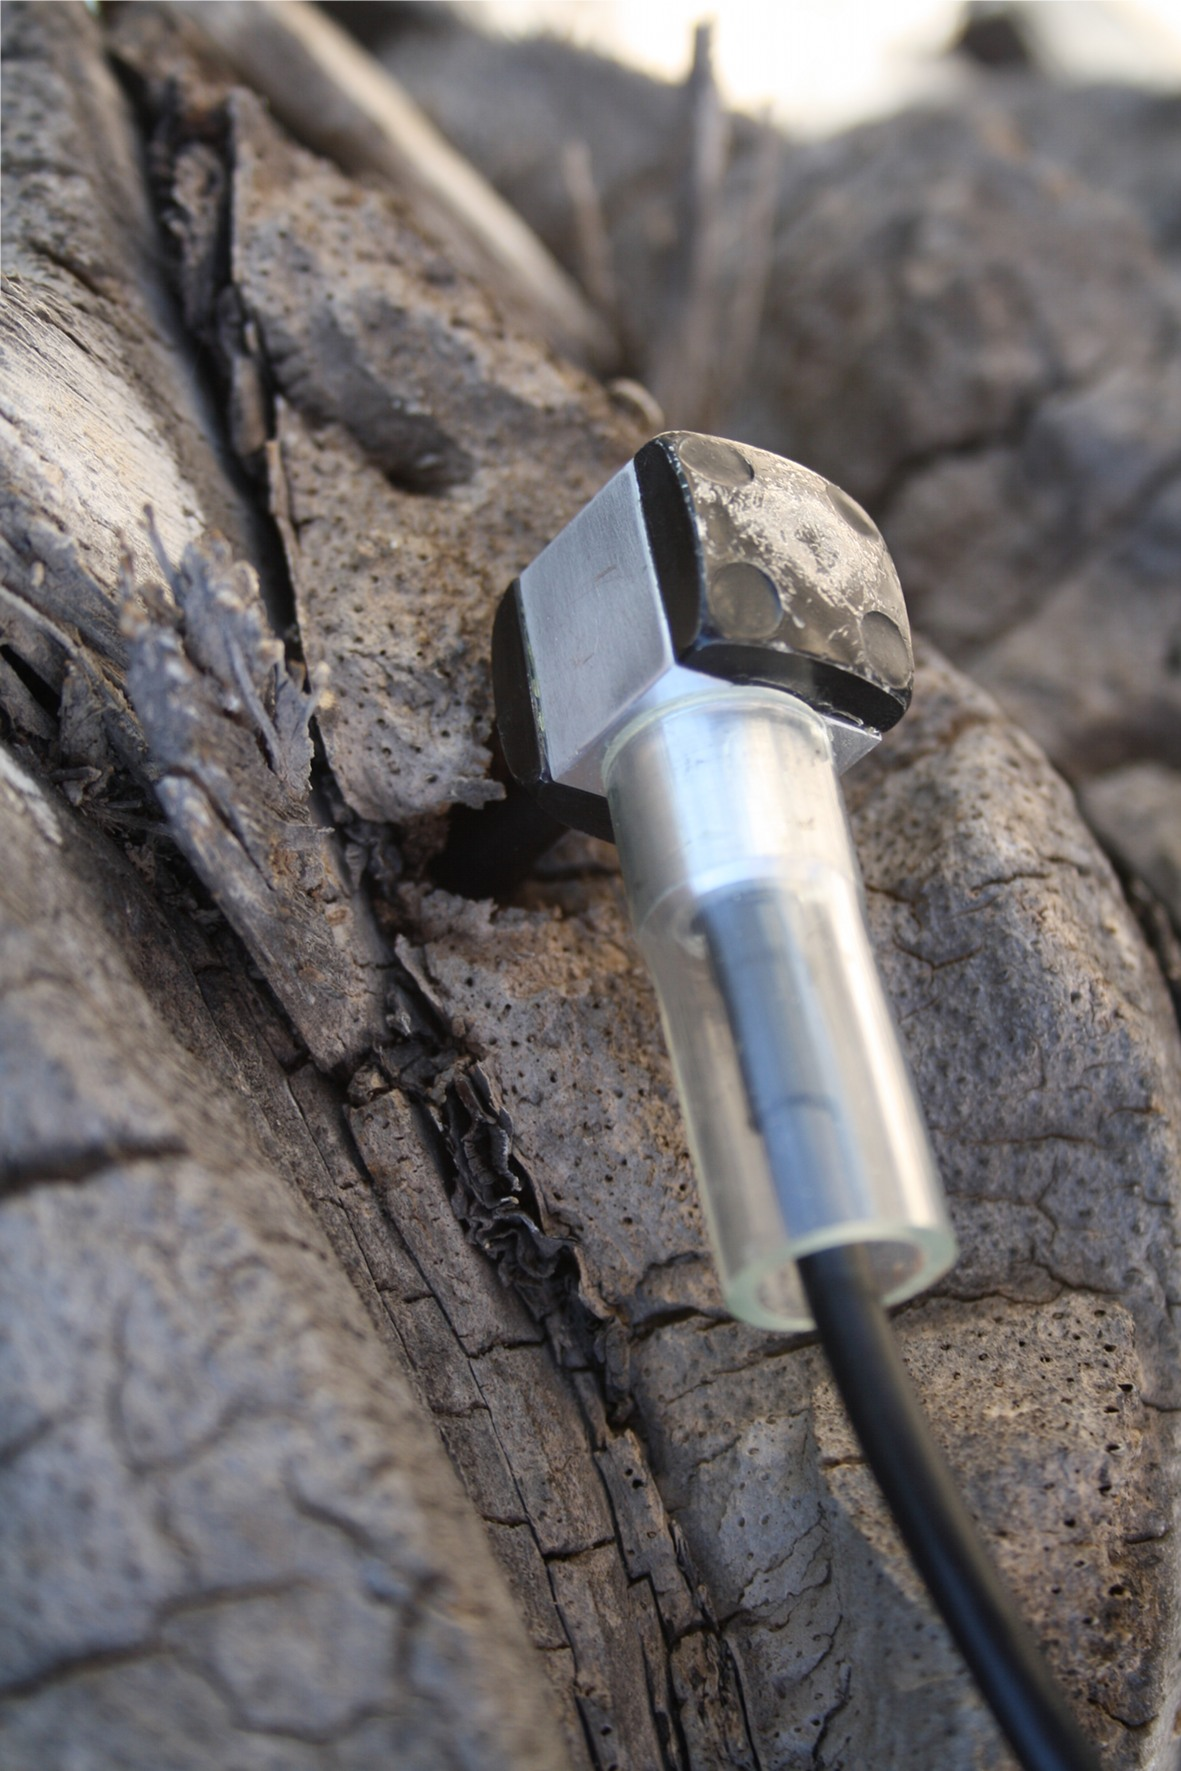
\includegraphics{gis-pfc-ch6-02.jpg}}
	\qquad
	\subfloat[Transductor utilizado como sensor][]{
	    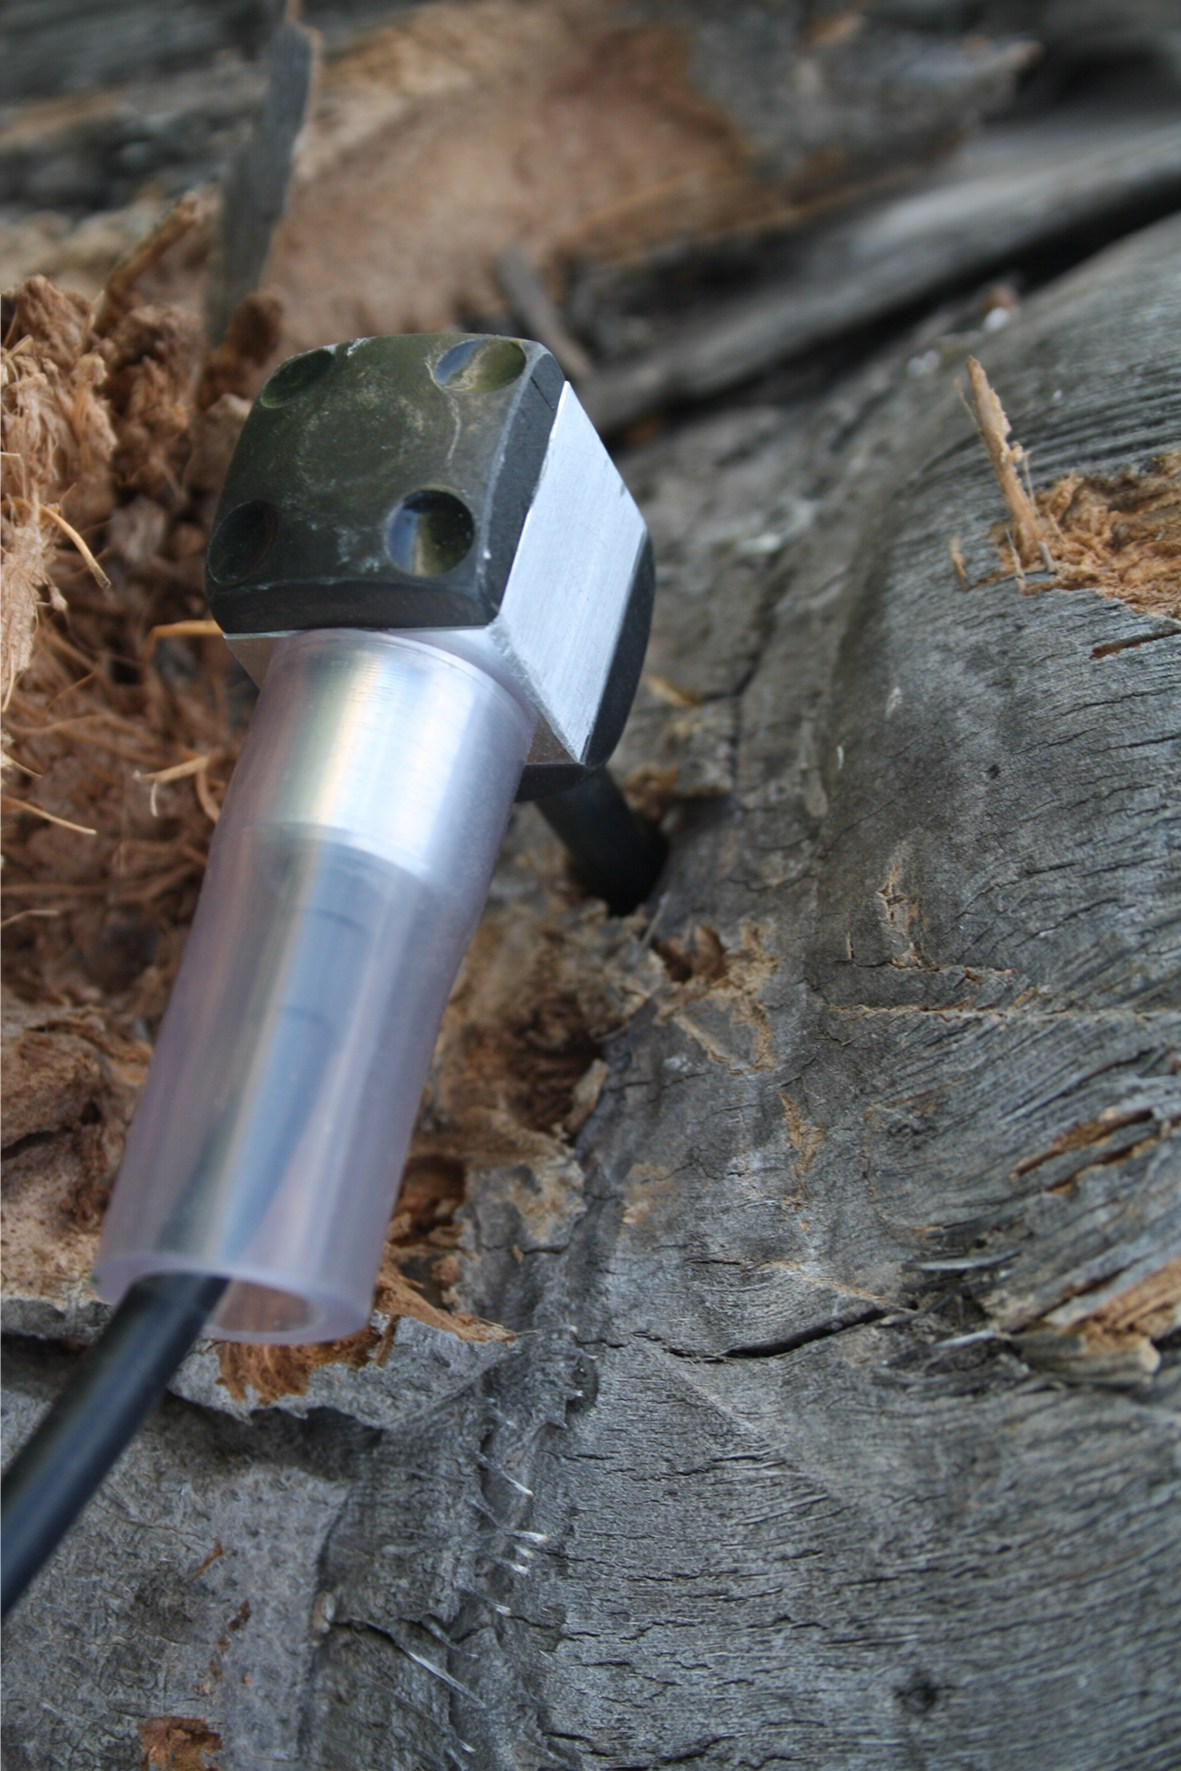
\includegraphics{gis-pfc-ch6-03.jpg}}
    \end{center}
    \caption[Transductores de impacto utilizados durante los
    ensayos]{Imágenes de los transductores tomadas durante la realización
    de los ensayos. Se aprecia la diferencia entre el transductor utilizado
    como actuador y el que se utiliza como sensor al observar las marcas
    que deja el martillo en la cabeza metálica del primero.}
    \label{fig:transducers}
\end{figure}

Este tipo de transductor puede utilizarse indistintamente como actuador o
como sensor ya que es la estructura metálica externa del transductor la
que, al recibir el golpe del martillo, genera y transmite la onda acústica.
Por su parte, el componente activo de la sonda realiza la transformación de
onda de presión a onda eléctrica y únicamente en este sentido\footnote{Es
fácil observar que el sentido de la conversión es único, puesto que la
sonda coaxial que conecta el sensor con el osciloscopio únicamente
transmite información en forma de señal eléctrica y únicamente en el
sentido que va del transductor al osciloscopio. Además es bien sabido que
los osciloscopios no generan señal alguna por sus canales de medida.}. Si
el transductor actúa como sensor envía una señal eléctrica correspondiente
con la onda acústica recibida, por el contrario, si sirve como actuador
transmite la correspondiente a la onda transmitida; de ese modo es fácil
registrar ambas señales.

En concreto los transductores utilizados en este proyecto fin de carrera
han sido fabricados por el fabricante húngaro de equipos para la
realización de pruebas no invasivas
\href{http://www.fakopp.com/site/piezo}{fakopp}. Se trata de transductores que,
pese a estar diseñados para resistir el impacto de un martillo, ofrecen una
buena relación señal a ruido. Funcionan a una frecuencia de resonancia
propia de 45 kHz (es menester recordar que la banda de actuación de los
ultrasonidos parte de los 20 kHz y llega a los 1000 MHz, por lo que una
frecuencia de 45 kHz es en este contexto una frecuencia relativamente
baja) adecuada para el tipo de ensayos que se desea realizar en este
apartado del proyecto.


\subsection{Resto de equipo utilizado}

A parte de los transductores, el equipo utilizado para la realización de
ensayos no destructivos en palmeras in vivo no difiere mucho del que
comúnmente se utiliza para ejecutar pruebas similares.

Para la adquisición de datos se ha utilizado un osciloscopio de laboratorio
conectado por medio de un enlace de red, en una comunicación par a par, a
un \sig{pc}. El propósito del \sig{pc} es el de almacenar las muestras que
se obtienen con el osciloscopio. Al emplear pulsos acústicos es preciso
configurar el disparo del osciloscopio apropiadamente (en base a la señal
transmitida), de lo contrario los pulsos transmitido y recibido salen
rápidamente de pantalla y apenas se perciben.

Para preparar el árbol para las pruebas se ha precisado de un taladro y una
azadilla. Las palmeras disponen de una corteza muy resistente y difícil de
penetrar formada por los restos de antiguas ramas que quedan después de que
éstas se poden. Al estar formada por madera <<muerta>>, la corteza de la
palmera puede alterar los resultados de las pruebas por lo que antes de
fijar los transductores es necesario limpiar una pequeña zona de la planta
y proporcionar acceso al verdadero tallo.

Los dispositivos electrónicos utilizados, así como el taladro mecánico,
precisan de suministro eléctrico para funcionar. Al realizarse las pruebas
en terreno abierto no existe otra alternativa que la de alimentar estos
instrumentos por medio de una batería. Sin embargo, las baterías generan
una tensión continua que no es compatible con los requisitos de aparatos
diseñados para proveerse de la red eléctrica, por lo tanto ha sido
necesario también el uso de un transformador de continua a alterna junto
con la batería. Además para gozar de cierta movilidad durante las pruebas
se ha hecho uso de una alargadera común.

El procedimiento para determinar la velocidad de propagación de la onda
ultrasónica comprende averiguar el tiempo de vuelo de la onda y medir el
espesor de la muestra, dividiendo estas dos magnitudes se obtiene la
velocidad de propagación. Medir el espesor del tallo de una palmera se hace
difícil con una cinta métrica, por no decir que las medidas tomadas son
poco precisas. Por este motivo para la realización de ensayos en los que se
desea registrar también el espesor del espécimen evaluado se fabrica un
calibre apropiado. El calibre de factura propia, mostrado en la
\cref{fig:calibre}, permite determinar de un modo significativamente más
sencillo y exacto el grosor del tallo.

\begin{figure}
    \begin{center}
	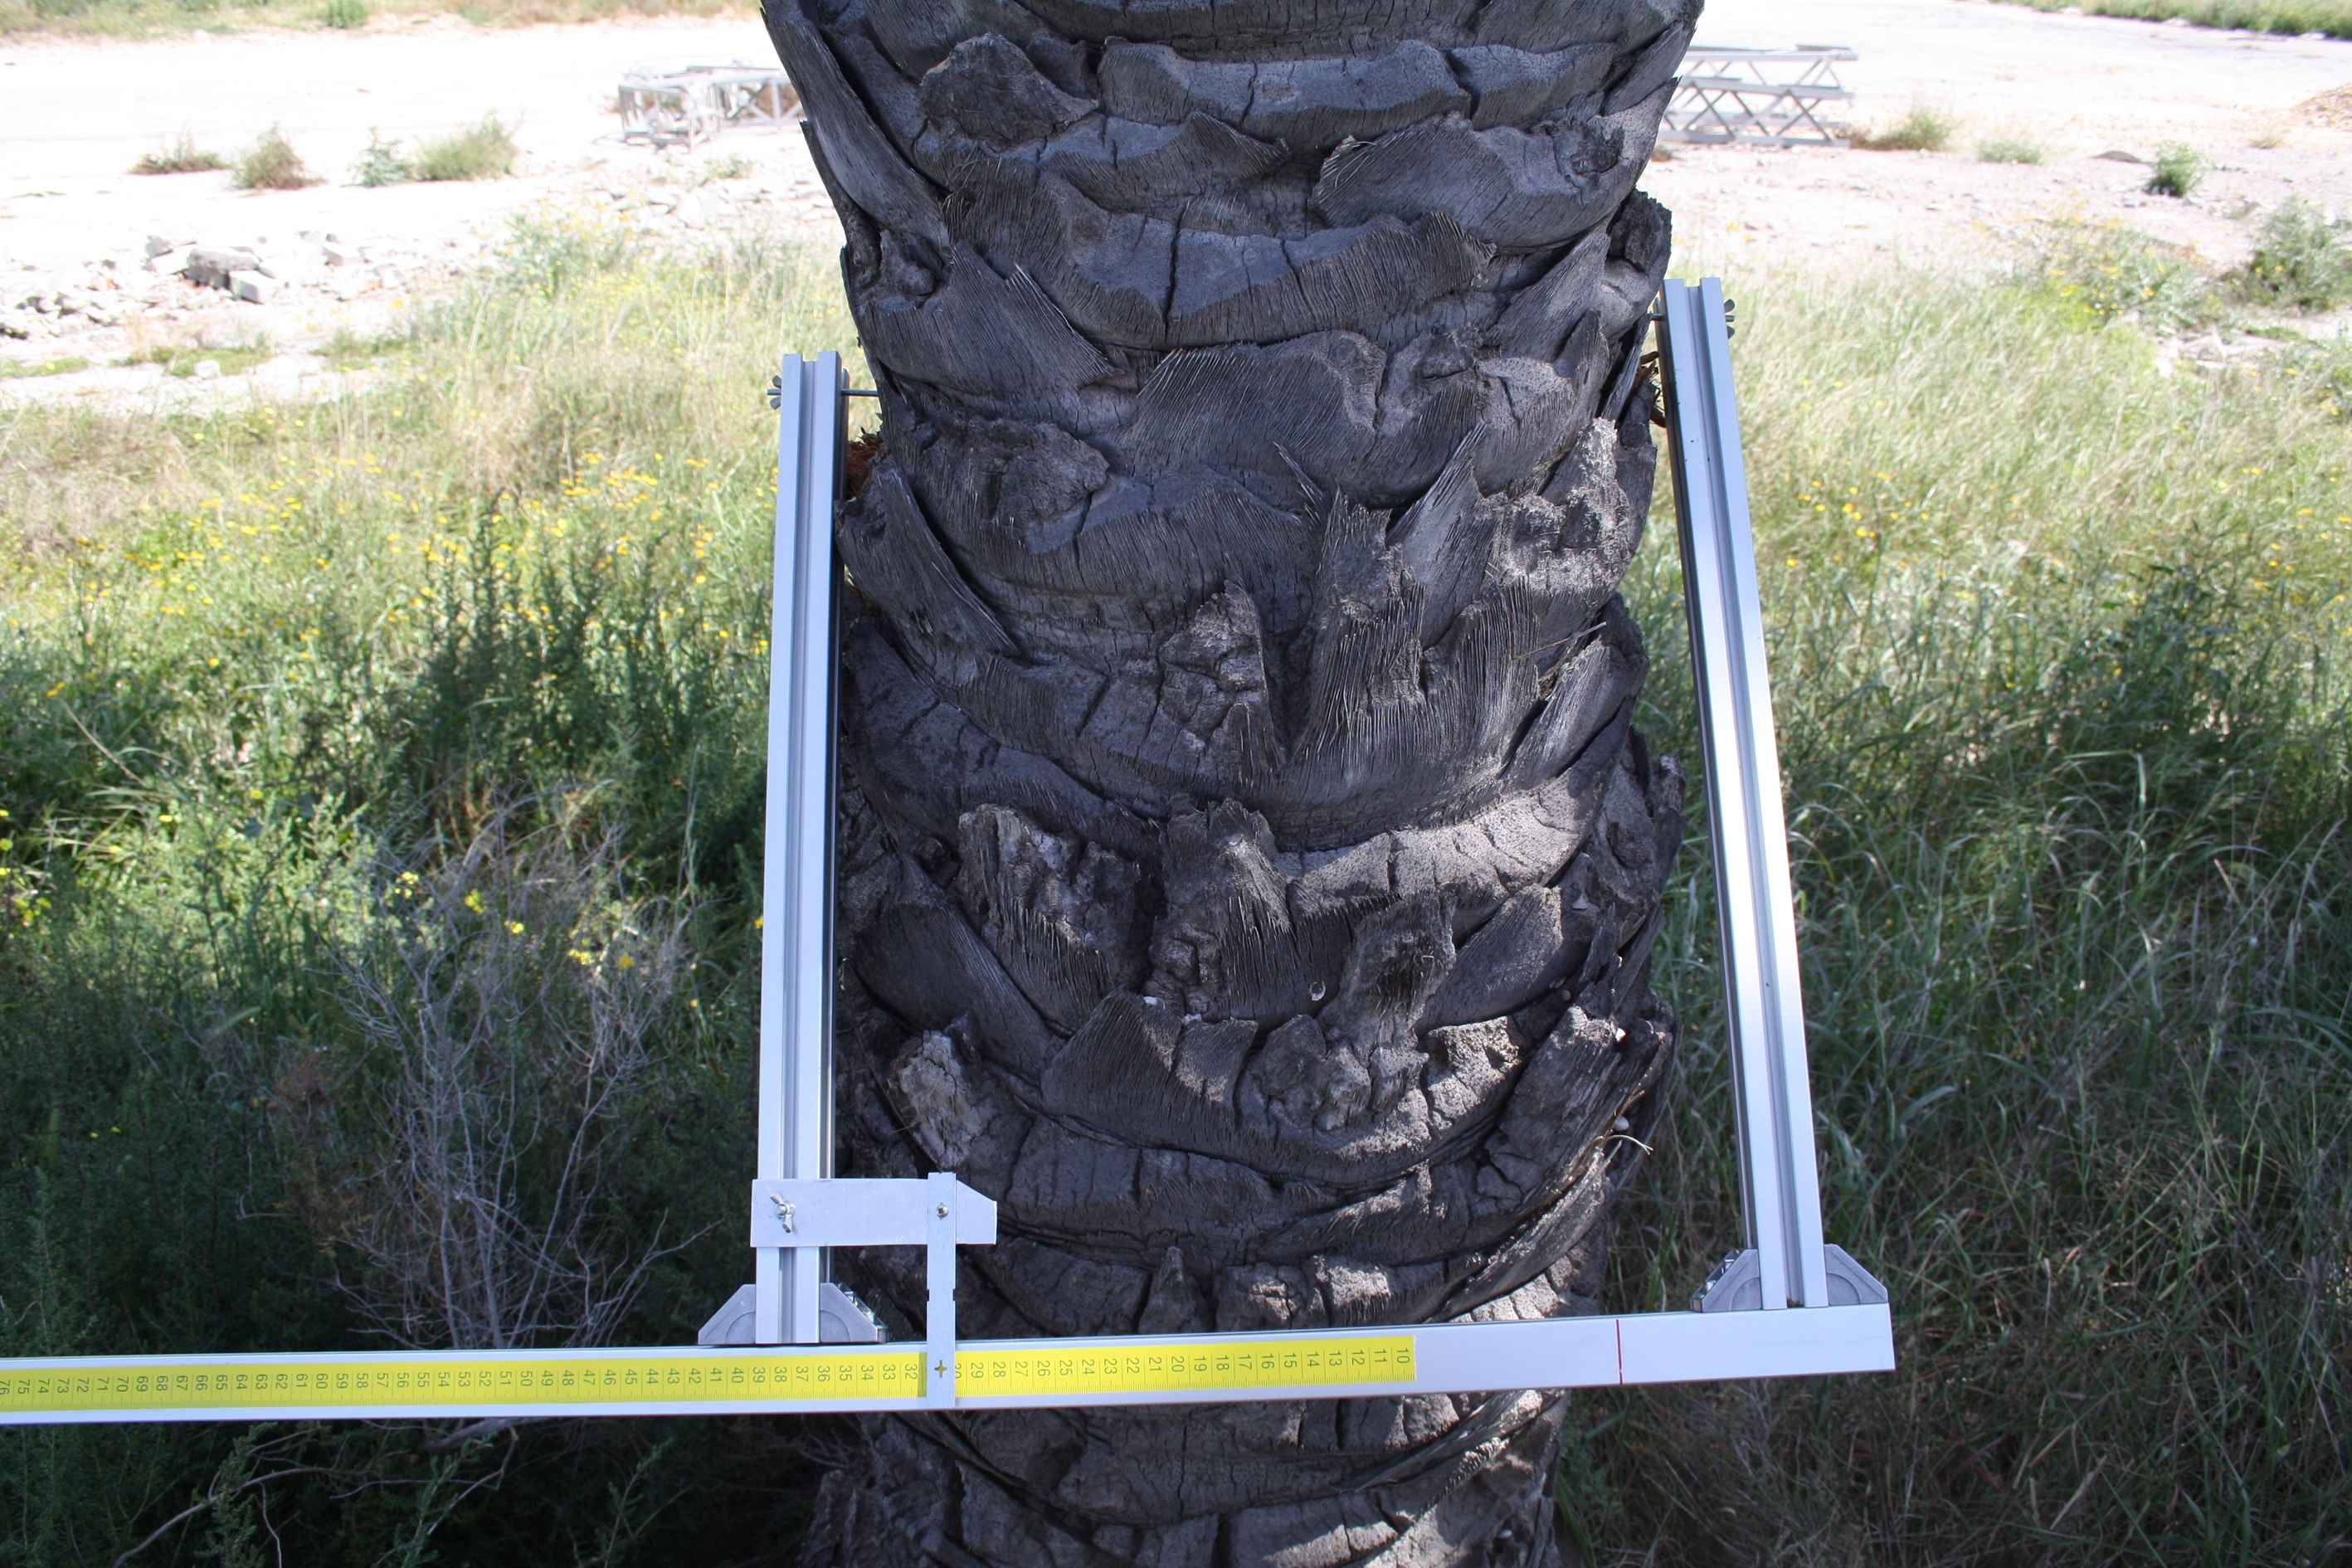
\includegraphics{gis-pfc-ch6-04.jpg}
    \end{center}
    \caption[Calibre en los ensayos]{Calibre construido a propósito de los
    ensayos realizados. Permite evaluar fácilmente y con mayor precisión el
    espesor de la muestra.}
    \label{fig:calibre}
\end{figure}

Para terminar se exponen aquí el resto de elementos incluidos en el equipo
utilizado, se trata principalmente de instrumentos utilizados para
registrar las dimensiones u otras características de las muestras: una
cinta métrica, una referencia y una cámara de fotos (para obtener un valor
aproximado de la altura total de la palmera comparando en las fotografías
realizadas la altura de las marcas situadas a distintos niveles en la
referencia, que es conocida, con la del ejemplar), un martillo para
percutir el sensor y en último lugar, pero no por ello menos importante,
bolígrafo y papel para realizar anotaciones.


\section{Metodología seguida durante las pruebas}\label{sec:methodology}

Las pruebas realizadas persiguen demostrar que existe una relación entre
los distintos parámetros de la señal recibida y las características del
medio en que se propaga. Si así fuese quedaría justificado un estudio más
ambicioso cuyo objetivo sería el de determinar de forma inequívoca dicha
relación. Los parámetros que se pretende evaluar para intentar dictaminar
que dicha relación en efecto existe son los listados a continuación:

\begin{itemize}
    \item Amplitud de la señal, para determinar en que medida se ha visto
	atenuada la onda sónica al propagarse.
    \item Aparición de dispersión, se evalúa si hay signos visibles del
	efecto de la dispersión en la onda recibida.
    \item Velocidad de propagación, el cociente del diámetro del ejemplar y
	el tiempo de vuelo ayudan a determinar la velocidad de propagación
	de la onda.
    \item Desplazamiento en frecuencia, se observa la posición del máximo
	del espectro frecuencial de la onda ultrasónica.
    \item Curva de atenuación, o forma de la señal, se evalúa si la caída
	de la señal es más o menos suave o abrupta.
    \item Aparición de secundarios, debidos a efectos varios como la
	propagación de onda superficial.
\end{itemize}

Estos parámetros se evalúan en los resultados recogidos al realizar
diferentes ensayos en muestras de distintos tipos, como son: palmeras
sanas, se toman muestras de palmeras ubicadas en distintas localizaciones,
realizando ensayos en ejemplares pertenecientes a múltiples variedades y
que presentan asimismo características variadas como grosor o tipo de
corteza; además se evalúa palmeras muertas o ejemplares que aparentan un
mal estado de salud, eucaliptos, pinos y, finalmente, postes de telefonía.
De ese modo es posible realizar una comparación posterior para tratar de
identificar una relación entre los parámetros estimados y las condiciones o
tipo de la muestra.

El lector ha de notar que no es posible extraer resultados válidos de
muestras de palmera en laboratorio. Ello es debido a que el tallo de la
palmera pierde sus propiedades originales cuando el ejemplar muere.
Mientras vive una palmera intercambia nutrientes y agua entre su copa y sus
partes basales a través de vasos que integran su tallo, principalmente
utilizando un mecanismo basado en la capilaridad. Al morir el individuo
este proceso se detiene y el tallo va perdiendo su composición húmeda
regularmente hasta que finalmente se seca por completo. Debido a esta otra
singularidad que presentan las palmeras, los resultados obtenidos en
muestras extraídas de los restos de un ejemplar no son confiables y no
aportan información válida para la finalidad de este estudio. Es por ello
por lo que los ensayos que aquí se han realizado en ejemplares, palmeras,
in vivo.

La relación entre las propiedades de la madera de palmera y los parámetros
de la señal evaluados es, como se ha afirmado anteriormente, desconocida;
pero no sólo eso, el modo en que las condiciones externas influyen en el
medio es también desconocido. Por último cabe destacar aquí, en parte para
el posterior entendimiento de las conclusiones y resultados expuestos en
este documento que: debido al motivo que se ha manifestado, carece de
sentido comparar los datos obtenidos de las ondas recibidas al realizar
ensayos en las distintas muestras siempre que no se haga en el contexto
---esto es, mirando también las características--- de la onda que parte del
emisor durante la realización de cada prueba.


\subsection{Procedimiento de medida}

Durante la realización de las pruebas se ha seguido un procedimiento
concreto con el objetivo de tomar las medidas de una forma ordenada. El
conjunto de pasos de que consta dicho procedimiento se expone aquí de
forma resumida.

\begin{enumerate}
    \item En primer lugar se ha de trasladar el equipo a las proximidades
	del ejemplar en el van a realizarse las medidas.
    \item Después se asienta una mesa (u otro soporte) y se dispone el
	equipo para la toma de muestras.
    \item Se conecta el transformador a la batería, la alargadera al
	transformador y el resto de equipos a las tomas de la alargadera.
    \item Se realiza la limpieza de la zona de inserción de las sondas con
	ayuda del taladro y la azadilla.
    \item Se mide el espesor del ejemplar y la altura del tallo a la que se
	van a realizar los ensayos y se anotan en la libreta.
    \item Se toma una fotografía del ejemplar situando la referencia en las
	proximidades.
    \item Se encienden los equipos electrónicos y se insertan los punzones
	de las sondas en el tallo del ejemplar.
    \item Por último se toman las medidas. Para ello, mientras una persona
	golpea el actuador la otra verifica que los ajustes del
	osciloscopio son correctos y realiza la transferencia de datos
	desde el osciloscopio hasta el \sig{pc}. Se recogen de entre cinco
	a siete muestras por ejemplar.
\end{enumerate}

La escala de amplitudes del osciloscopio se ajusta del siguiente modo.
Durante la realización de los ensayos a la primera palmera se fija la
escala de amplitudes de modo que la señal recibida ocupe toda la pantalla,
pudiendo observar así los rasgos de la señal en mayor detalle. Sin embargo,
para poder comparar en igualdad de condiciones onda transmitida y onda
reflejada se mantiene la misma escala para la onda transmitida lo que
ocasiona que parte de la onda transmitida quede fuera del monitor del
osciloscopio. Al recoger los datos, todo aquello que queda fuera de la
ventana del osciloscopio se descarta, ello origina que señales de mayor
amplitud aparezcan truncadas en las figuras expuestas en el apartado de
resultados de este capítulo. A efectos de comparar varias señales
únicamente se ha de observar que cuando una señal aparece truncada es
porque es de una magnitud mayor que una que no lo está. Este mismo concepto
se ha de aplicar también al comparar medidas de varias muestras, ya que
para poder comparar los resultados de forma ecuánime se ha mantenido la
escala de amplitudes del osciloscopio durante la ejecución de todos los
ensayos.

Se muestra a continuación la \cref{fig:tests}, aparecen en ella dos
fotografías tomadas durante la ejecución de los ensayos. Estas fotografías
complementan la descripción que se ha hecho de los pasos que comprende el
procedimiento de toma de medida, de modo que el lector pueda comprender
mejor como se han realizado los ensayos. La primera de las figuras muestra
una palmera que, a juzgar por el tamaño que ocupa en la figura en
comparación con las dimensiones de la referencia se calcula que debe medir
unos $5.5$ metros altura aproximadamente. La segunda muestra a su vez una
palmera de medidas similares y parte del equipo utilizado dispuesto para la
toma de muestras.

\begin{figure}
    \begin{center}
	\subfloat[Palmera de unos $5.5$ metros de alto a juzgar por su
	    tamaño en la fotografía en comparación con el de la
	    referencia.][]{
	    \begin{minipage}[c]{.425\textwidth}\label{fig:testheight}
		\centering
		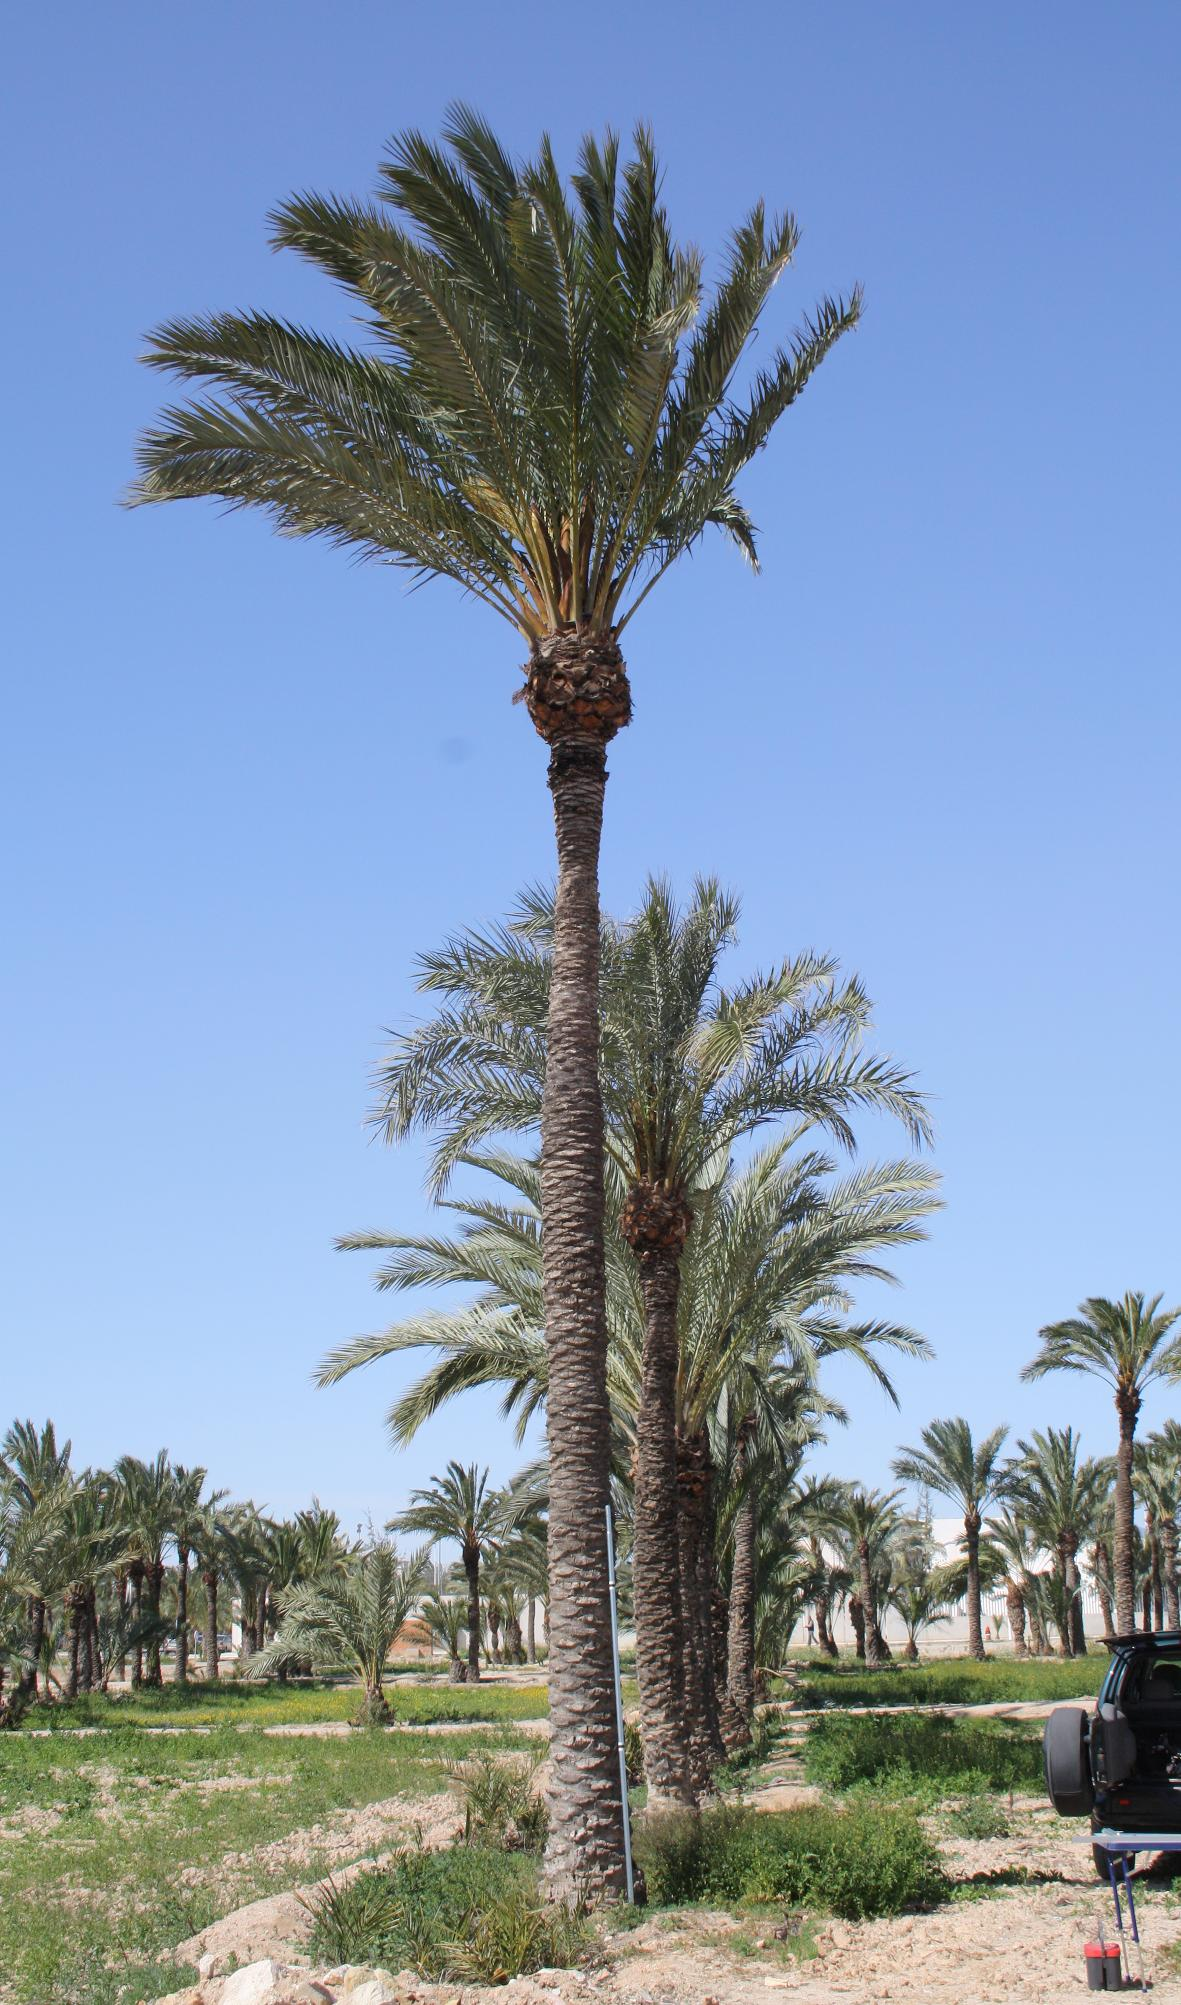
\includegraphics{gis-pfc-ch6-05.jpg}
	    \end{minipage}}
	\subfloat[Fotografía en la que se observa parte del equipo de
	    medida utilizado.][]{
	    \begin{minipage}[c]{.425\textwidth}\label{fig:testequipment}
		\centering
		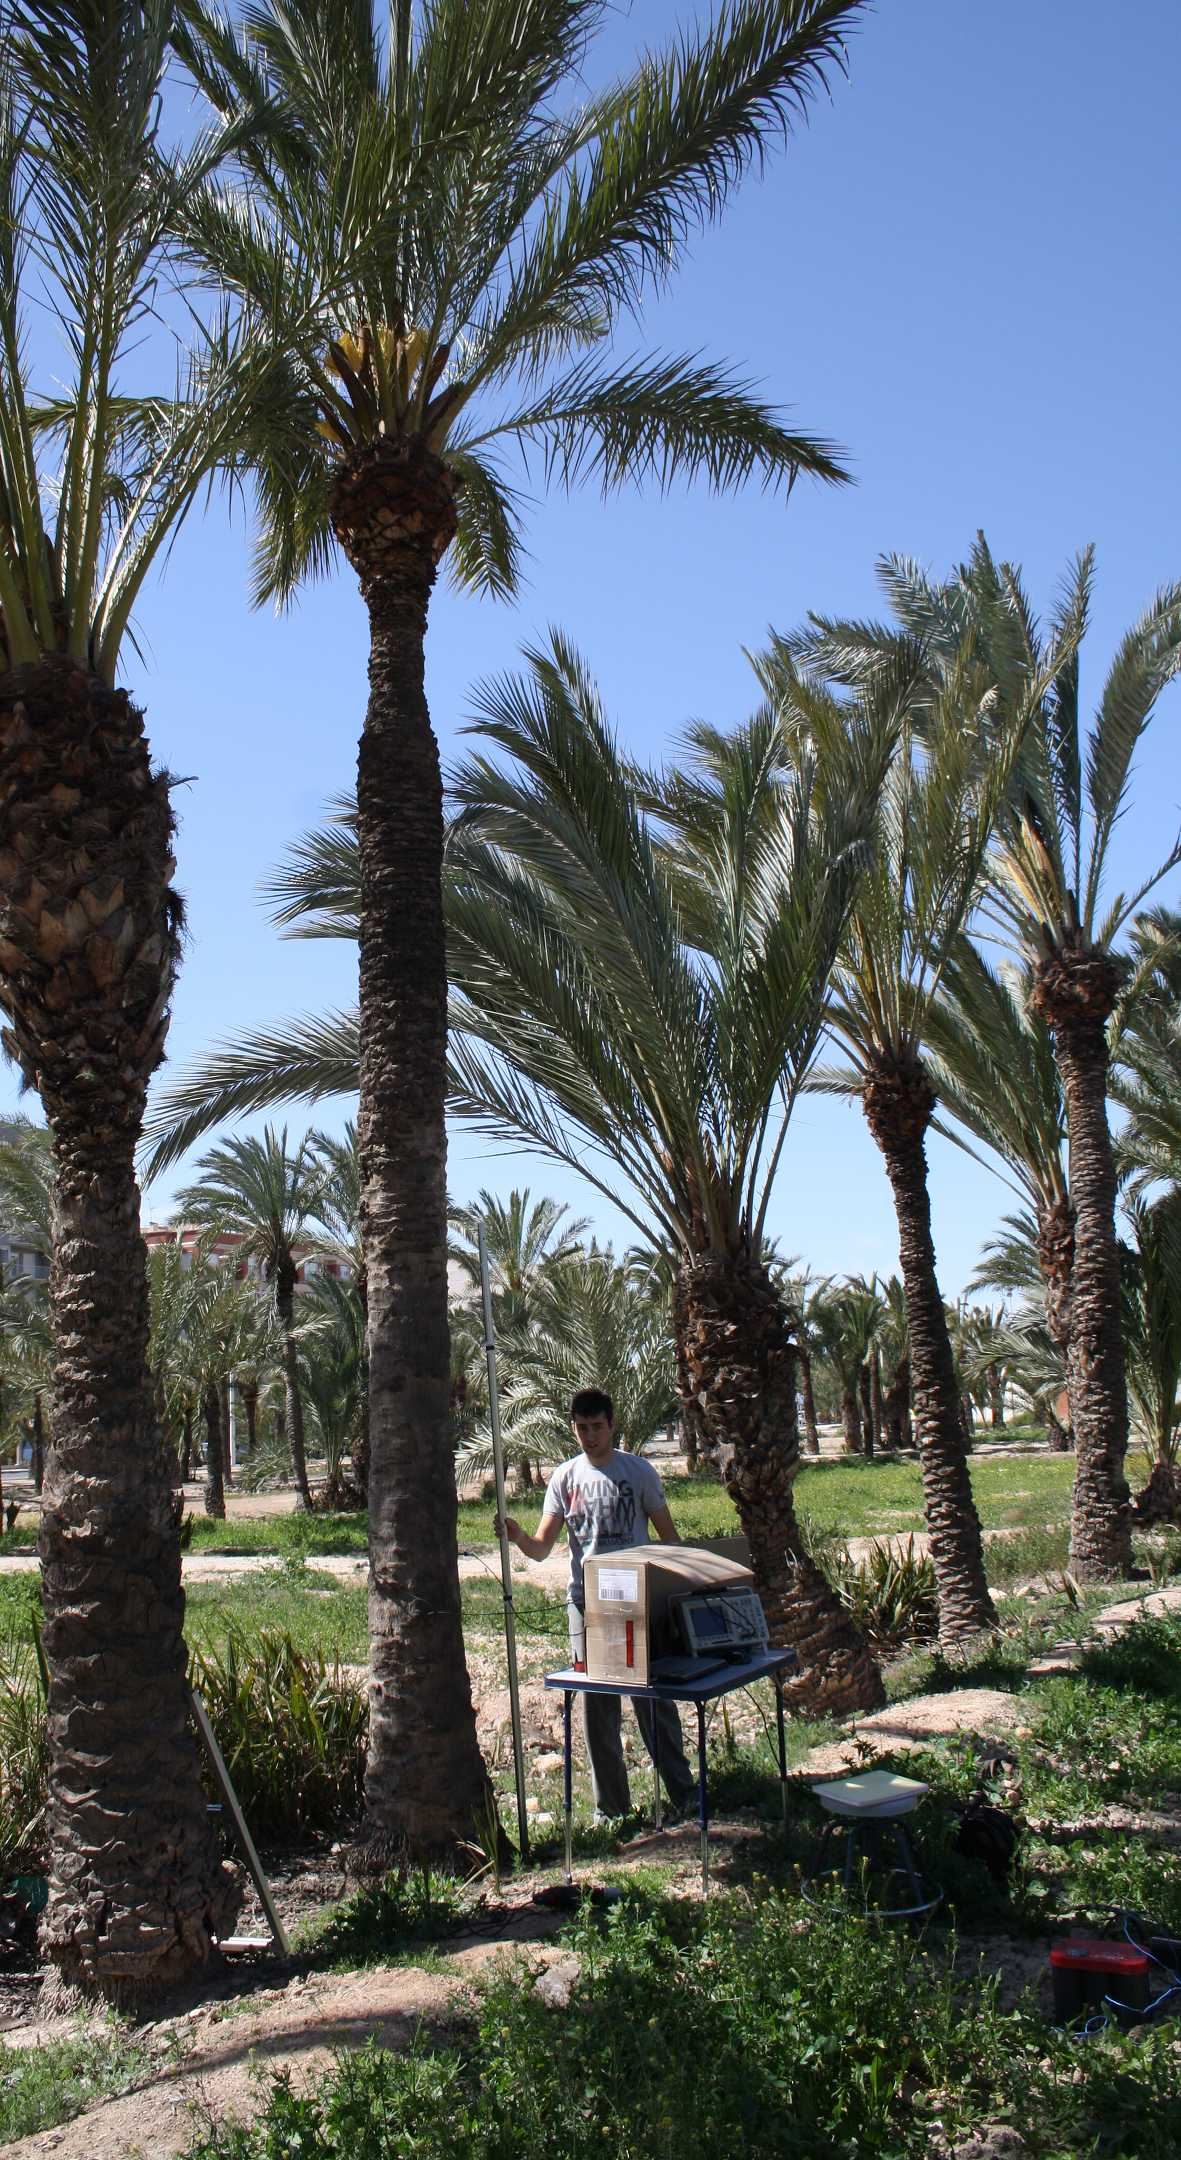
\includegraphics{gis-pfc-ch6-06.jpg}
	    \end{minipage}}
    \end{center}
    \caption[Fotografías tomadas durante la realización de los
    ensayos]{Fotografías tomadas durante la realización de los ensayos.}
    \label{fig:tests}
\end{figure}


\subsubsection{Inconvenientes surgidos durante la toma de medidas}

El procedimiento de medida ha resultado tedioso y complejo no sólo por el
hecho de que el procedimiento que ha de ejecutarse para tomar las muestras
es largo, complejo y fatigoso; si no también debido a los siguientes
motivos.

En primer lugar, al realizarse medidas de campo, es preciso trasladarse a
la ubicación en la que se encuentra localizada la muestra para poder
realizar las medidas. Las muestras potenciales, por su naturaleza, se
encuentran en terreno de difícil acceso como zanjas o huertos, a los que es
preciso trasladar el voluminoso equipo para poder realizar las medidas. En
cada ocasión se ha de desplazar el equipo hasta las proximidades de la
muestra y después dicho equipo debe disponerse de modo que el ensayo pueda
ser realizado. Tarea que no siempre es fácil, debido ---como se ha dicho---
a la naturaleza del terreno que frecuentemente resulta irregular y
accidentado, con lo cual la simple acción de asentar una mesa se convierte
en complicada.

Por otro lado, gran parte del equipo utilizado requiere de alimentación
eléctrica para funcionar, al operar en lugares apartados se ha precisado de
una batería para alimentar los distintos dispositivos utilizados. La
capacidad de la batería es limitada lo que limita la duración de una sesión
de toma de muestras. Además, al agotarse es preciso detener las pruebas
durante el periodo de recarga de la batería, que dura aproximadamente un
día, antes de poder reemprender los ensayos.

A todo ello debe añadirse que tanto el director como el proyectista en este
proyecto fin de carrera desconocían previamente a los ensayos el manejo de
los transductores de impacto que se han empleado para la realización de las
pruebas, lo cual ha dificultado, más aún si cabe, la ejecución de los
ensayos.


\section{Resultados obtenidos}

Tras finalizar el proceso de medida se dispone de 420 muestras, entre ondas
ultrasónicas transmitidas y recibidas, que ha habido que procesar para
poder observar como se comportan los parámetros de la señal sometidos a
observación (véase la \vref{sec:methodology}) en las distintas condiciones
en las que se han realizado los ensayos. Para ello se han desarrollado
rutinas en \matlab{} que permiten realizar las siguientes operaciones:
% (210 correspondientes a ondas acústicas transmitidas y otras 210
% correspondientes a las respectivas ondas recibidas)

\begin{itemize}
    \item Importar las señales transmitida y recibida, y la duración
	temporal de las mismas a partir de los archivos de muestras.
    \item Calcular la media aritmética de todas las muestras (distinguiendo
	entre onda transmitida y recibida) tomadas de un mismo ejemplar.
    \item Realizar el cálculo de la \sig{fft} de cada muestra individual y
	de la media obtenida en el paso anterior.
    \item A partir de las señales en el dominio temporal y las señales en
	el dominio espectral representar gráficos acompañados de curvas
	auxiliares en los que pueda compararse la señal transmitida (o su
	espectro) con la señal recibida (o su espectro).
    \item Cálculo automático de tiempos de vuelo y desplazamiento del
	máximo en frecuencias.
\end{itemize}

Las figuras a continuación y el \cref{tab:results} muestran los valores
observados en las muestras más representativas del conjunto, aquellas que
muestran más claramente los fenómenos que se ponen de relieve más adelante,
en los siguientes párrafos.

\begin{table}
    \centering
    \begin{tabular}{ld{1,3}d{2,2}d{4,2}d{2,1}d{2,2}}
	\toprule
	\multicolumn{1}{c}{Muestra} &
	\multicolumn{1}{c}{Altura (m)} &
	\multicolumn{1}{c}{Espesor (cm)} &
	\multicolumn{1}{c}{$V_p$ ($\text{ms}^{-1}$)} &
	\multicolumn{1}{c}{$\Delta f$ (kHz)} \\
	\midrule
	Palmera sana (i) & 1,13 & 45 & 515,58 & 24,9 \\
	Palmera sana (ii) & 1,1 & 36 & 739,73 & 20,3 \\
	Palmera sana (iiia) & 1,04 & 41,8 & 508,67 & 18,1 \\
	Palmera sana (iiib) & 1,43 & 33 & 986,84 & 28,7 \\
	Palmera muerta & 1,2 & 30,5 & 851,16 & 1,91 \\
	Eucalipto & 1,165 & 31 & 1374,1 & 32,25 \\
	Pino & 1,165 & 37,75 & 1337,9 & 3,83 \\
	Poste telefónico & 1,15 & 21,7 & 1379,9 & 5,75 \\
	\bottomrule
    \end{tabular}
    \caption[Tabla comparativa de resultados]{Tabla comparativa donde
    aparecen los resultados obtenidos a partir de las muestras más
    significativas (la segunda columna contiene la altura a la que se han
    tomado las muestras).}
    \label{tab:results}
\end{table}

Por lo general, exceptuando alguna muestra concreta, se observa lo
siguiente: a medida que una madera es más maciza y presenta menor grado de
humedad, se observa que las ondas sónicas se propagan más rápidamente por
ella (compárese en el \cref{tab:results} la velocidad de propagación,
$V_p$, para las distintas muestras) y se ven menos afectadas por la
atenuación; asimismo en maderas <<secas>> y compactas los ultrasonidos
sufren una menor dispersión y sufren menor desplazamiento espectral (véase
el desplazamiento del máximo del espectro en frecuencias, $\Delta f$, en el
mismo cuadro).

La \cref{fig:velfreq} muestra para cada ejemplar la relación entre la
velocidad de propagación de la onda y el desplazamiento del máximo
frecuencial, en dicha gráfica puede observarse lo siguiente: las marcas
correspondientes a palmeras sanas (se refiere a medidas tomadas a una
altura similar ---\atr{Pal1}, \atr{Pal2} y \atr{Pal3a}---) se encuentran
agrupados en la misma zona de la gráfica lo que significa que la onda
ultrasónica se propaga a velocidades similares y muestra desplazamientos
del máximo frecuencial parejos, en general, la velocidad de propagación en
palmeras es pequeña y el desplazamiento que sufre el máximo frecuencial
elevado; por su parte las ondas ultrasónicas se propagan rápidamente por
pinos (\atr{Pin}) y postes (\atr{Pos}) telefónicos, además al propagarse
por estos medios no sufre tanto $\Delta f$; se observa también como las
medidas tomadas en la palmera muerta (\atr{Palm}) y a una altura superior
en una palmera sana (\atr{Pal3b}) difieren claramente de las obtenidas en
palmeras sanas a la altura convencional; por último, la onda ultrasónica se
propaga rápidamente en eucaliptos (\atr{Euc}) pero también muestra un
elevado desplazamiento en frecuencias.

\begin{figure}
    \begin{center}
	\includegraphics{gis-pfc-ch6-17.pdf}
    \end{center}
    \caption[Comparación de la $V_p$ y el $\Delta f$ para las distintas
    muestras.]{Comparación de la velocidad de propagación y el
    desplazamiento del máximo frecuencia para las distintas muestras.}
    \label{fig:velfreq}
\end{figure}

Véase como este fenómeno se pone de manifiesto al comparar, por ejemplo,
las \cref{fig:eucalipto,fig:palmera1} que representan la onda recibida en
un eucalipto y la onda recibida en una palmera sana respectivamente. Las
\cref{fig:eucalipto-transmitida,fig:palmera1-transmitida} representan por
su parte sus respectivos pares transmitidos. Se observa que, aunque la
duración de la onda transmitida en el eucalipto es mayor que la de la
transmitida a la palmera, la duración de la onda recibida en la palmera
supera a la de la recibida en el eucalipto. Eso significa que la señal se
ensancha o se dispersa más al propagarse por madera de palmera, cuyo
contenido en agua es elevado, que al propagarse por madera de eucalipto,
más compacta. Además se puede ver como la señal recibida en el eucalipto
sale de los límites del osciloscopio y satura, mientras que la recibida en
la palmera se ve comparablemente atenuada.

\begin{figure}[p]
    \begin{center}
	\includegraphics{gis-pfc-ch6-07.pdf}
    \end{center}
    \caption[Eucalipto (onda recibida)]{Eucalipto, onda recibida (el tiempo
    se mide en segundos y la amplitud en voltios).}
    \label{fig:eucalipto}
\end{figure}

\begin{figure}[p]
    \begin{center}
	\includegraphics{gis-pfc-ch6-10.pdf}
    \end{center}
    \caption[Primera palmera sana (onda recibida)]{Primera palmera sana,
    onda recibida (el tiempo se mide en segundos y la amplitud en
    voltios).}
    \label{fig:palmera1}
\end{figure}

\begin{figure}[p]
    \begin{center}
	\includegraphics{gis-pfc-ch6-08.pdf}
    \end{center}
    \caption[Eucalipto (onda transmitida)]{Eucalipto, onda transmitida.}
    \label{fig:eucalipto-transmitida}
\end{figure}

\begin{figure}[p]
    \begin{center}
	\includegraphics{gis-pfc-ch6-11.pdf}
    \end{center}
    \caption[Primera palmera sana (onda transmitida)]{Primera palmera sana,
    onda transmitida.}
    \label{fig:palmera1-transmitida}
\end{figure}

En maderas más blandas la señal recibida se compone de una sola
contribución o eco o en ocasiones de varios, sólo que solapados, en parte
debido a la acción de la dispersión que al ensanchar los ecos causa el
solapamiento. Por el contrario en maderas más sólidas se aprecia la
frecuente aparición de ecos secundarios que aparecen mejor definidos en la
señal recibida. Obsérvese este fenómeno al comparar los resultados
expuestos en las \cref{fig:pino-recibida,fig:palmera2-recibida} que
corresponden a los resultados al evaluar un pino y otra de las palmeras
sanas respectivamente.

\begin{figure}[p]
    \begin{center}
	\includegraphics{gis-pfc-ch6-15.pdf}
    \end{center}
    \caption[Pino (onda recibida)]{Pino, onda recibida.}
    \label{fig:pino-recibida}
\end{figure}

\begin{figure}[p]
    \begin{center}
	\includegraphics{gis-pfc-ch6-12.pdf}
    \end{center}
    \caption[Segunda palmera sana (onda recibida)]{Segunda palmera sana,
    onda recibida. Se observa una discontinuidad en la forma de la señal
    que puede ser debida a la presencia de un eco secundario que solapa con
    la contribución principal.}
    \label{fig:palmera2-recibida}
\end{figure}

En cuanto al desplazamiento en frecuencia, se aprecia que a medida que una
madera es más compacta el desplazamiento del máximo del espectro en
frecuencias decrece. Esto puede verse si se compara por ejemplo el
desplazamiento observado en el espectro de las señales correspondientes a
una palmera y a un poste telefónico,  --figuras--. Obviamente queda patente
al contemplar los resultados que el desplazamiento es mayor al desplazarse
la onda por la palmera.

Por último, para finalizar este apartado, se muestran las muestras tomadas
de los siguientes ejemplares: \cref{fig:palmeramuerta-recibida},
correspondiente a una muestra tomada de una palmera muerta; las
\cref{fig:palmera3a-recibida,fig:palmera3b-recibida} representan los datos
obtenidos al evaluar una palmera a diferentes alturas, primero más abajo y
luego más arriba; la última figura del grupo, la \cref{fig:poste-recibida},
representa por su parte el aspecto de la señal recibida al efectuar el
ensayo en un poste telefónico. Puede observarse como la curva
correspondiente a la palmera muerta es más compacta que la del resto de
palmeras, se puede ver como conserva su forma y al mismo tiempo no presenta
la aparición de ecos secundarios. Al observar los resultados obtenidos a
distintas alturas en una misma palmera se infiere que la madera de un
ejemplar vivo es más seca y compacta a medida que se asciende por el tallo,
pero para confirmarlo deberían realizarse más medidas en distintos
ejemplares. Las muestras tomadas de un poste telefónico revelan una señal
recibida caótica, plagada de ecos secundarios, pero a pesar de ello no
demasiado dispersa.

\begin{figure}[p]
    \begin{center}
	\includegraphics{gis-pfc-ch6-09.pdf}
    \end{center}
    \caption[Palmera muerta (onda recibida)]{Palmera muerta, onda
    recibida.}
    \label{fig:palmeramuerta-recibida}
\end{figure}

\begin{figure}[p]
    \begin{center}
	\includegraphics{gis-pfc-ch6-13.pdf}
    \end{center}
    \caption[Tercera palmera sana (onda recibida)]{Tercera palmera sana,
    medida a menor altura, onda recibida.}
    \label{fig:palmera3a-recibida}
\end{figure}

\begin{figure}[p]
    \begin{center}
	\includegraphics{gis-pfc-ch6-14.pdf}
    \end{center}
    \caption[Tercera palmera sana (onda recibida)]{Tercera palmera sana,
    medida a mayor altura, onda recibida.}
    \label{fig:palmera3b-recibida}
\end{figure}

\begin{figure}[p]
    \begin{center}
	\includegraphics{gis-pfc-ch6-16.pdf}
    \end{center}
    \caption[Poste telefónico (onda recibida)]{Poste telefónico, onda
    recibida.}
    \label{fig:poste-recibida}
\end{figure}


\section{Conclusiones y futuras líneas de trabajo}

A juzgar por los resultados obtenidos en este estudio preliminar se infiere
que existe en efecto una relación entre los parámetros de la señal obtenida
en un ensayo por ultrasonidos y las características, ya sean físicas o
estructurales, de un ejemplar de palmera in vivo. Sin embargo, la ausencia
de un profundo estudio teórico previo a la realización de las pruebas
impide extraer conclusiones significativas de los resultados obtenidos. Es
por ello que se recomienda la ejecución en un futuro próximo de un proyecto
más ambicioso en este campo que permita determinar sin ambigüedad que
relación existe, creyendo suficientemente justificado este proyecto en
vistas a los resultados que se han expuesto en esta memoria.


\part*{Apéndices}

\appendix
\addtocounter{totalpages}{\value{page} + 1}		       % totalpages
\pagenumbering{bychapter}					% chappg
\chapter{Gu�a de usuario de la aplicaci�n de control}\label{chap:appendixA}

Es sabido que el prop�sito de una memoria de proyecto fin de carrera es exponer los procedimientos mediante los cuales se aborda un determinado tema de investigaci�n, dar a conocer los frutos obtenidos en la ejecuci�n de los mismos y alcanzar una serie de conclusiones a partir de esos resultados. Por tanto, la inclusi�n del manual de usuario del software de representaci�n de se�ales y espectros en frecuencia se aleja de las pretensiones convencionales de una memoria de \textsc{pfc}. No obstante, la aplicaci�n inform�tica se ha desarrollado durante el curso del proyecto y forma parte del mismo. Adem�s, cabe la posibilidad de que suscite inter�s en un p�blico que encuentre de poca utilidad el resto del texto. Teniendo �sto en consideraci�n, se ha cre�do conveniente la adici�n del manual al documento pero en forma de ap�ndice al final de �ste.\par
Este manual est� destinado a todo aquel usuario interesado en la representaci�n de se�ales el�ctricas en el contexto que se ha expuesto anteriormente en el libro. En concreto, puede ser de especial inter�s para aquellos usuarios que deseen representar el espectro en frecuencia de una se�al el�ctrica en tiempo real, de forma que al mismo tiempo pueda visualizarse la se�al correspondiente a dicho espectro.\par
Los objetivos que pretende esta gu�a son: en primer lugar, ofrecer una visi�n general de la aplicaci�n que hace hincapi� en el aspecto de la interfaz y en las posibilidades del software; en segundo lugar se dan unas pautas para facilitar el proceso de adaptaci�n del usuario a la interfaz que muestra la aplicaci�n; pero, puesto que el uso de la aplicaci�n es sencillo, el verdadero prop�sito de esta gu�a es servir de manual de consulta que permita recordar en caso de olvido cual es con detalle la funcionalidad de los elementos que componen la interfaz de usuario.


\section{Un vistazo general de la interfaz de usuario}

En la \vref{fig:interface} puede observarse el aspecto general (justo despu�s de ejecutarse y antes de ser utilizada) que muestra la aplicaci�n de control. Como puede verse, se ha dividido la interfaz gr�fica en distintos paneles en los que se re�nen los elementos de que consta esta interfaz. En el primer panel se observan los elementos que permiten controlar los par�metros de configuraci�n de la tarjeta de adquisici�n. Un segundo panel contiene un monitor en el que se representan los resultados del proceso de adquisici�n en los modos num�ricos o no visuales de funcionamiento de la aplicaci�n. Adem�s, un subpanel alberga los controles que permiten, por un lado, gobernar el modo de funcionamiento y, por otro, el comportamiento de la funci�n de representaci�n.

\begin{figure}
	\begin{center}
		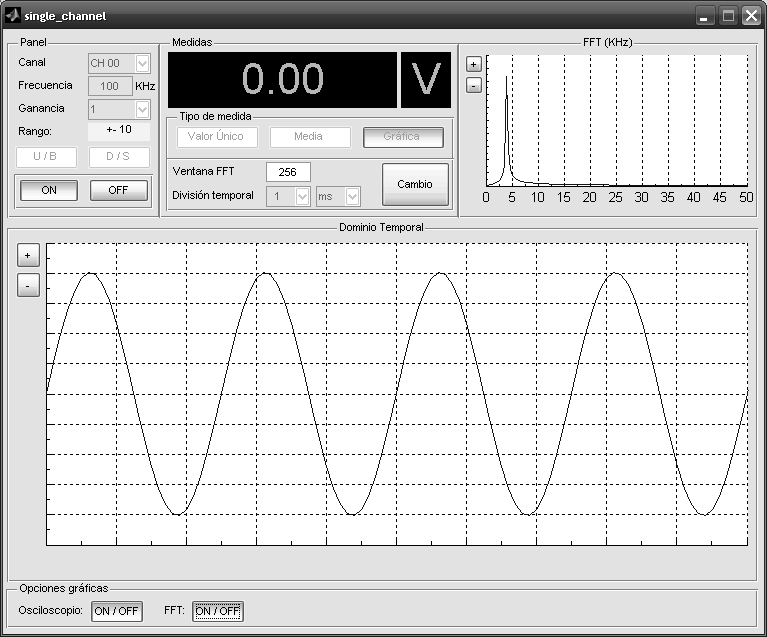
\includegraphics{gis-pfc-appa-01.png}
	\end{center}
	\caption[Aspecto de la interfaz con controles y gr�ficos separados por paneles]{Aspecto de la interfaz con controles y gr�ficos separados por paneles.}
	\label{fig:interface}
\end{figure}

A continuaci�n pueden observarse dos paneles que contienen los espacios de coordenadas destinados a alojar las representaciones de se�al y espectro y varios grupos de controles, uno por cada espacio de coordenadas, cada uno de los cuales controla propiedades del espacio de coordenadas al que est� sujeto. Por �ltimo, un quinto panel dispone de los mandos necesarios para habilitar o deshabilitar la representaci�n de se�al, espectro o ambos.


\section{Especificaciones t�cnicas y limitaciones}

A continuaci�n se enumeran brevemente los requisitos necesarios para poder emplear la aplicaci�n de control.

\begin{itemize}
	\item En primer lugar es necesario un \textsc{pc} funcionando sobre el sistema operativo Microsoft Windows.
	\item En dicho \textsc{pc} debe encontrarse correctamente instalada una tarjeta \kpci{} o similar. Son compatibles con la aplicaci�n las tarjetas fabricadas por \emph{Keithley} que dispongan al menos de un puerto de adquisici�n anal�gica, cuyas caracter�sticas sean similares a la \kpci{} y cuya interacci�n con la \datx{} de \matlab{} sea similar a la interacci�n que se da entre este software y la \kpci{}. Para que una tarjeta de adquisici�n de datos se encuentre correctamente instalada en un \textsc{pc}, en primer lugar debe encontrarse correctamente conectada a la placa base del \textsc{pc} y, en segundo lugar, deben haberse instalado con �xito los drivers de la misma.
	\item Para poder emplear el software resulta imprescindible que en el \textsc{pc} correspondiente se halle instalada una copia de la suite matem�tica \matlab{} cuya versi�n sea compatible con la aplicaci�n.
	\item Es necesario tener acceso desde \matlab{} a los ficheros correspondientes a la aplicaci�n de control que, como es obvio, tendr�n que haberse instalado previamente en el \textsc{pc}.
	\item Es necesaria una interfaz externa compatible con los conectores mini-\sig{d} de la \kpci{}. Puede emplearse por ejemplo la caja de conexiones descrita en el \vref{subsec:conbox}, en ese caso ser� necesaria al menos una sonda en la que, por lo menos, una de las terminaciones sea compatible con la caja de conexiones.
\end{itemize}

Como indica su t�tulo, este apartado se ha pensado adem�s para indicar las limitaciones que muestra la aplicaci�n de control. Desde el punto de vista de su origen estas limitaciones pueden dividirse en limitaciones derivadas del uso de la \kpci{} y en limitaciones introducidas por la propio software. Para una mayor informaci�n sobre las primeras pueden consultarse las \vrefrange{sec:technical}{subsec:throughput} en el segundo cap�tulo. A destacar el comportamiento del rendimiento de la tarjeta que se ver� reducido seg�n se vayan a�adiendo canales al objeto dispositivo.\par
En cuanto a las limitaciones que introduce el software son las siguientes. Para empezar es destacable el hecho de que �nicamente es posible controlar un canal de muestreo desde la aplicaci�n de control. El canal controlado puede estar asociado a cualquier puerto f�sico de la tarjeta pero s�lo se da acceso a un �nico canal por sesi�n. A esta limitaci�n se debe a�adir que desde el software es imposible crear o eliminar canales u objetos dispositivo de forma manual.\par
Por otro lado se da la incapacidad de modificar desde la utilidad propiedades de la configuraci�n de la tarjeta que no vengan representadas por controles en la interfaz de usuario. Algunos de estos controles se deshabilitan durante la actividad de muestreo, se ha hecho as� para impedir que se altere el valor de par�metros tales como la frecuencia de muestreo en tiempo real. En ocasiones es \matlab{} desde un nivel superior en la jerarqu�a del software el que impide que una de estas propiedades cambie al vuelo, en el resto de casos se ha hecho para evitar problemas de rendimiento experimentados durante pruebas de software.\par


\section{Instrucciones de uso}

El manejo del software de representaci�n de se�ales es relativamente sencillo. Para arrancar el software debe ejecutarse en primer lugar \matlab{}\footnote{Si se necesita m�s informaci�n con respecto al uso de \matlab{}, puede consultarse el manual de instrucciones proporcionado por el desarrollador del software.}. Despu�s debe hacerse una llamada a la aplicaci�n de control, existen tres modos de hacer esto mismo, todos ellos explicados con detalle en el manual de usuario de \matlab{}. En lo fundamental el procedimiento es id�ntico a la llamada a una funci�n implementada en un fichero de c�digo de \matlab{}. De los modos mencionados son interesantes desde la perspectiva que adopta este manual dos de ellos.\par

\begin{itemize}
	\item El primero, quiz�s m�s intuitivo, es el modo gr�fico, que m�s bien es un compendio de las distintas formas de ejecutar un fichero *.m que permite \matlab{}, s�lo que aplicado al c�digo de una aplicaci�n con interfaz de usuario. Para dar un ejemplo, desde el navegador de carpetas de \matlab{} puede hacerse click con el bot�n derecho del rat�n en el fichero *.m asociado al software (fichero \texttt{single\_channel.m}) y seguidamente seleccionar en el desplegable que aparece la opci�n <<ejecutar archivo>>.
	\item Otra forma es la llamada desde la l�nea de comandos. Cercior�ndose de que el directorio actual contiene los ficheros \texttt{single\_channel.m} correspondiente al c�digo y \texttt{single\_channel.fig} correspondiente a la distribuci�n de la interfaz puede escribirse en la l�nea de comandos la orden:

		\begin{lstlisting}[gobble=16]
			[handles = ]single_channel[(opciones)]
		\end{lstlisting}

	Siendo la parte entre corchetes del comando opcional.\par Lo interesante de este m�todo es que permite el acceso a las propiedades internas y objetos de los que hace uso la aplicaci�n de control. De este modo es posible a partir del objeto \texttt{handles} tener acceso, por ejemplo, al objeto dispositivo que controla la tarjeta de adquisici�n de se�ales. Adem�s a trav�s de la llamada por l�nea de comandos es posible pasar argumentos para posibles opciones relacionadas con las interfaces de usuario.
\end{itemize}

De no existir ning�n objeto dispositivo asociado a la \kpci{}, la funci�n de creaci�n presente en la aplicaci�n crea, al iniciarse �sta, un objeto dispositivo asociado a la \kpci{} o cualquier otra tarjeta fabricada por \emph{Keithley} soportada por el software e instalada en el \textsc{pc}. En caso contrario el software hereda uno de los posibles objetos dispositivos existentes a�adiendo un nuevo canal y emite un mensaje de advertencia.\par
Al cerrar la aplicaci�n se detiene el proceso de muestreo y, si el n�mero de canales pertenecientes al objeto dispositivo empleado no ha disminuido, se elimina el canal cuyo orden corresponde al n�mero de canales existentes al lanzar la aplicaci�n m�s uno. Es importante remarcar que en ning�n caso se elimina el objeto dispositivo del que se ha hecho uso, ni siquiera cuando es la aplicaci�n la que lo ha generado. Queda pues en manos del usuario la tarea de destruir cualquier canal creado por la aplicaci�n de control y el objeto dispositivo correspondiente en caso de ser necesario. La forma m�s sencilla de hacerlo es la que se cita a continuaci�n, que tambi�n eliminar� cualquier variable que quedase en el espacio de trabajo de \matlab{} ---para evitarlo debe llamarse a \texttt{clear} utilizando como argumentos, separados por espacios entre ellos y del comando, los nombres de los objetos dispositivos eliminados de la memoria de \matlab{} que queden en el espacio de trabajo---.

\begin{lstlisting}
	delete(daqfind);
	clear;
\end{lstlisting}


\subsection{Descripci�n detallada de la interfaz de usuario}

Aqu�, en este apartado, se muestran los controles y sus funciones para que el usuario pueda comprender su funcionamiento. Para facilitar la b�squeda se ha procedido a agrupar las definiciones empleando como criterio la pertenencia a mismo panel, es decir, todos los controles que aparecen reunidos en un mismo panel en la interfaz de usuario se explican en un mismo cuadro.

\begin{table}
	\centering
	\begin{minipage}{.85\textwidth}
		\begin{description}
			\item[Canal] Determina el puerto f�sico asociado al canal en uso. Se trata de un control desplegable que se expande mostrando todos los puertos seleccionables.
			\item[Frecuencia] Permite ajustar la frecuencia de muestreo. La nueva frecuencia de muestreo se limita de forma autom�tica de modo que se encuentre entre 1 kHz y la m�xima frecuencia de muestreo permitida por la tarjeta.
			\item[Ganancia] Ajusta el rango de amplificaci�n del amplificador de instrumentaci�n integrado en la tarjeta. Esto a su vez condiciona la amplitud de pico m�xima de la se�al que entra a la \kpci{}. �ste es tambi�n un control desplegable y muestra el conjunto de ganancias posibles.
			\item[Rango] Indicador que presenta el rango en el que debe mantenerse la amplitud de la se�al que entra a la tarjeta para que el conversor anal�gico digital no sature dada una configuraci�n de ganancia y m�todo de adquisici�n. Puede consultarse el \vref{tab:acqmodes} al respecto.
			\item[Control u/b] Controla el modo de adquisici�n en el proceso de muestreo. El modo de adquisici�n es en la \datx{} una propiedad del objeto dispositivo y no del canal.
			\item[Control d/s] Permite configurar el modo de terminaci�n correspondiente al canal que se controla. De configurarse como diferencial el listado de canales que muestra el desplegable \textsf{canal} se modifica para concordar con esta configuraci�n.
		\end{description}
	\end{minipage}
	\caption[Descripci�n del primer panel de controles]{Descripci�n del primer panel de controles.}
	\label{tab:first-panel}
\end{table}

El primer panel descrito en el \vref{tab:first-panel} alberga un panel secundario o subpanel en el que se encuentran ubicados dos controles m�s. Estos controles son el control \emph{on} y el control \emph{off} que respectivamente sirven para iniciar o detener el proceso de muestreo.\par
El siguiente panel a la derecha con el nombre de \emph{medidas} muestra un indicador num�rico verde en fondo negro que, una vez activado el proceso de muestreo, si la aplicaci�n se encuentra funcionando en los modos \emph{valor �nico} o \emph{media}, presenta el valor que toma la se�al en cada evento. Adicionalmente puede verse un panel m�s peque�o, \emph{tipo de medidas}, dentro de este panel. Los elementos que incorpora el subpanel tipo de medidas vienen explicados en el \vref{tab:second-panel}.

\begin{table}
	\centering
	\begin{minipage}{.85\textwidth}
		\begin{description}
			\item[Tipo de medidas] Representado por tres botones: \emph{valor �nico}, \emph{media}, y \emph{gr�fica}; de los cuales s�lo uno puede quedar pulsado al mismo tiempo. Gobierna el modo de funcionamiento del software de control. Los modos de funcionamiento de la aplicaci�n de control se encuentran explicados al detalle en el \vref{subsec:working-modes}.
			\item[Ventana fft] Determina la longitud en n�mero de muestras de la ventana empleada para el c�lculo de la \textsc{fft}. Este control se presenta en la forma de cuadro de texto editable. El valor introducido en el texto es redondeado a la siguiente potencia de dos.
			\item[Divisi�n temporal] Este mando est� formado por dos controles desplegables. El primero de los cuales permite seleccionar un n�mero de una secuencia que va de 1 a 400. El segundo por su parte sirve para seleccionar una escala de unidades: milisegundos o microsegundos. El prop�sito del conjunto es controlar la longitud temporal que representa el eje de coordenadas del espacio de coordenadas en el que se representa la se�al. Esto que a priori parece no repercutir demasiado en el funcionamiento del software, adquiere una gran importancia dado que el software de control se ha dise�ado para asemejarse en su modo de funcionamiento gr�fico a un osciloscopio digital. Para m�s informaci�n sobre el funcionamiento de los osciloscopios digitales cons�ltese el \vref{subsec:repmodes}.
			\item[Cambio] Inicialmente la \textsc{fft} de la se�al se representa en el espacio de coordenadas m�s peque�o, arriba a la derecha en la interfaz de usuario, y la se�al se representa en el espacio de coordenadas mayor. Mediante este mando es posible reubicar las representaciones de se�al y transformada de Fourier.
		\end{description}
	\end{minipage}
	\caption[Descripci�n del segundo panel de controles]{Descripci�n del segundo panel de controles incluido en el panel \emph{medidas}.}
	\label{tab:second-panel}
\end{table}

Para terminar existe un panel adicional que incorpora los controles \emph{osciloscopio} y \emph{fft}. Sendos mandos permiten en el modo de funcionamiento gr�fico habilitar o inhabilitar la representaci�n de la se�al y/o el c�lculo y representaci�n de la \textsc{fft} de la se�al respectivamente. Asimismo, cada uno de los paneles en los que se sit�an los espacios de coordenadas est� dotado de dos controles con una etiqueta que representa los signos matem�ticos de la suma y la resta. Estos botones controlan la escala axial en relaci�n con el eje de ordenadas en el espacio de coordenadas al que acompa�an.


\subsection{Modos de funcionamiento}\label{subsec:working-modes}

Los modos de funcionamiento que soporta el software de control de la \kpci{} son tres. En el �ltimo de ellos, el modo gr�fico, la aplicaci�n consigue simular un osciloscopio digital de acuerdo con los resultados mostrados en la \vref{sec:working-test}. Se han discutido los pormenores de este modo de funcionamiento a lo largo del grueso de la memoria, para evitar reiteraciones innecesarias no volver� a tratarse el tema en este punto.\par
El resto de modos de funcionamiento podr�a catalogarse como modos num�ricos o no gr�ficos. La raz�n es que durante el proceso de adquisici�n el usuario percibe un valor num�rico y no una representaci�n gr�fica de la se�al si alguno de estos modos se encuentra activado. Es importante destacar que estos modos de funcionamiento no son apropiados para el estudio de se�ales de alta frecuencia. En situaciones en las que la se�al oscila a alta frecuencia el an�lisis mediante la aplicaci�n configurada para funcionar en alguno de estos dos modos aporta informaci�n confusa que no debe ser tomada en cuenta. No obstante, se recomienda encarecidamente su uso de producirse la situaci�n contraria, aquella en la que la se�al analizada oscila con lentitud. Esto es debido en principio a la naturaleza de los algoritmos en los que se basan ambos modos de funcionamiento y los resultados que otorgan.\par % en cuanto a que aportan en tales circunstancias / en tal caso informaci�n confusa acerca de la se�al / se�ales / informaci�n no representativa.
Los modos num�ricos de funcionamiento comparten una mec�nica similar, en lo fundamental id�ntica, no obstante, diferente en cuanto a implementaci�n. La idea es programar, antes de que d� inicio el proceso de adquisici�n, los eventos relacionados con el objeto dispositivo de la \datx{} de modo que ocurran peri�dicamente. Cuando acontece uno de los eventos se obtiene un n�mero real a partir de una interpretaci�n hecha a partir de la muestra o muestras adquiridas desde el evento anterior y se escribe �ste en el indicador num�rico que forma parte de la interfaz de usuario. Hasta ah� las coincidencias entre los m�todos que ejecuta cada modo de funcionamiento.\par % de modo cada cierto n�mero peri�dico de muestras obtenidas se programan
Las diferencias entre el m�todo \emph{valor �nico} y \emph{media} son las que siguen:

\begin{itemize}
	% \item En primer lugar, con el modo valor �nico se obtiene el valor de la muestra adquirida justo antes, despu�s de producirse el evento, mientras que el modo media proporciona la media aritm�tica de las muestras obtenidas desde el evento inmediatamente anterior al actual al ritmo especificado por el control \textsf{frecuencia}.
	\item En primer lugar, en el modo valor �nico el software muestra en el display\footnote{A partir de la vig�simo tercera edici�n del diccionario de la real academia de la lengua se considera correcto decir visualizador e incorrecto decir \emph{display}.} el valor correspondiente a la muestra obtenida justo despu�s de producirse el �ltimo evento, mientras que el modo media proporciona la media aritm�tica de las muestras obtenidas desde el evento inmediatamente anterior al actual al ritmo especificado por el control \textsf{frecuencia}.
	\item M�s all� de lo inferido a partir del nombre de los modos, estos se diferencian en el criterio empleado en la definici�n del periodo entre eventos y en la herramienta que genera dichos eventos. El m�todo valor �nico emplea el reloj interno de la \kpci{} a modo de temporizador, los eventos en este modo se programan para que sucedan cada cuarto de segundo. Por el contrario el modo media emplea una especie de testigo electr�nico que implementa la \datx{} y que produce un evento cada vez que se adquiere un determinado n�mero de muestras definido por el usuario de \matlab{}, en este caso el programador, a trav�s de la propiedad \textsf{SamplesAcquiredFcnCount}. El n�mero de muestras que debe adquirirse antes de que se produzca un evento se ha configurado a un valor que queda entre la cantidad de muestras que se obtienen en 250 milisegundos a la frecuencia de muestreo establecida y un m�nimo que \matlab{} actualiza al modificarse esta frecuencia.
	\item Por �ltimo, cabe hacer menci�n al procedimiento empleado para obtener el valor que se muestra por pantalla. El modo valor �nico emplea la funci�n \texttt{getsample} que extrae una �nica muestra de la tarjeta de adquisici�n, de este forma la tarjeta pasa gran parte del periodo entre eventos en reposo. El modo media, por el contrario, utiliza la funci�n \texttt{mean} sobre \texttt{getdata} que recupera las muestras almacenadas hasta el momento en el buffer en tanto que lo borra.
\end{itemize}


\subsubsection[Modos num�ricos y se�ales de alta frecuencia]{Incompatibilidades entre los modos de funcionamiento num�ricos y el an�lisis de se�ales de alta frecuencia}

La raz�n de que estos modos de funcionamiento no sean apropiados para el estudio de se�ales de alta frecuencia es diferente seg�n el modo.

\begin{itemize}
	% \item El modo valor �nico extrae una muestra de la se�al de manera peri�dica. Si consideramos que la se�al resultante de este proceso es el producto entre la se�al analizada y un tren de deltas. Si combinamos el hecho de que la frecuencia de la se�al es superior o muy superior a la frecuencia del tren de deltas y que posiblemente no sea un m�ltiplo de �sta con la certeza de que ambas se�ales se encuentran desfasadas en una medida desconocida y que es dif�cil seguir un n�mero real que cambia cuatro veces por segundo, el resultado es una informaci�n ca�tica y poco representativa de la se�al.  % Dependiente del modo pero radica en la forma de obtener el n�mero que se muestra por pantalla. El primer m�todo aplicado a una se�al que oscila no en fase con la se�al de muestreo hace parecer el comportamiento de la se�al err�tico. El segundo, la media de muchos periodos de una se�al centrada en el origen tiende a cero.
	\item El modo valor �nico extrae una muestra de la se�al de manera peri�dica, con un periodo de un cuarto de segundo. Es decir, se muestrea la se�al a una frecuencia de muestreo de 4 Hz. Considerando la condici�n de que la frecuencia de la se�al muestreada es muy alta, puede considerarse como consecuencia la hip�tesis de que sea muy superior a la frecuencia de muestreo, adem�s es poco probable que la primera sea un m�ltiplo de la segunda. Si se combina esta suposici�n con la certeza de que el instante en el que empieza el muestreo no coincide con el instante en el que se origina la se�al, puede llegarse a la conclusi�n de que la informaci�n presentada en el visor es, empleando el modo valor �nico en el an�lisis de se�ales r�pidas, ca�tica, cuanto menos confusa y poco representativa de la se�al. % ambas frecuencias pueden no estar relacionadas por una raz�n de multiplicidad. Si combinamos el hecho de que la frecuencia de la se�al muestreada es muy superior a la frecuencia de muestreo, con la posibilidad probable de que la frecuencia de la se�al no sea un m�ltiplo de la frecuencia de muestreo, con la certeza de que el instante en el que empieza el muestreo no coincide con el instante en el que se origina la se�al.
	\item En el caso del modo media ocurre que la media de una cantidad determinada de periodos de una se�al peri�dica tiende m�s a cero cuanto m�s periodos de la se�al se estiman al calcular la media. Por tanto, si la frecuencia de la se�al es mucho mayor que la frecuencia con la que se actualiza el valor num�rico mostrado por pantalla, y �sta tambi�n est� en torno a 4 Hz, el valor que se obtiene es el cero.
\end{itemize}

No es que el modo de funcionamiento gr�fico de la aplicaci�n de control carezca de utilidad en el an�lisis de se�ales de baja frecuencia, si no que carece de utilidad pr�ctica. Debe recordarse al lector que el modo de funcionamiento gr�fico de la aplicaci�n sobre la que trata este manual pretende emular un osciloscopio digital en su modo de funcionamiento gr�fico y, como consecuencia, este modo de funcionar adolece de los problemas propios de este tipo dispositivos como por ejemplo el que se expone en este p�rrafo. El modo de representaci�n que adopta un osciloscopio digital para representar se�ales lentas es el modo de representaci�n continuo, dada la incapacidad de la funci�n de disparo del modo convencional de trabajar con este tipo de se�ales \footnote{Esto queda suficientemente explicado en el \vref{subsec:repmodes}.}. Este modo no aporta informaci�n visual precisa sobre la frecuencia de la se�al analizada ni sobre su valor de pico a pico. Por si fuera poco dada la implementaci�n que se le ha dado en esta aplicaci�n consume muchos m�s recursos que el modo de representaci�n convencional\footnote{De hecho en las pruebas de software que se han realizado para este proyecto el modo de representaci�n continuo no funciona excepto en el modo de depuraci�n de errores pausando la ejecuci�n del software, si bien es cierto las pruebas se realizaron con un \textsc{pc} poco actualizado.}. Y, como es obvio, el modo gr�fico independientemente del modo de representaci�n adoptado necesita m�s recursos de los que requieren el resto de modos de funcionamiento.\par
Es por esta raz�n por la que los modos num�ricos obtienen un mayor protagonismo en el an�lisis de se�ales de baja frecuencia, porque aportan una informaci�n lo bastante buena, comparable a la que proporciona el modo gr�fico, y consumen menos recursos que esta alternativa.



\backmatter

\addtocounter{totalpages}{\value{page} - 1}		       % totalpages
\pagenumbering{arabic}
\setcounter{page}{\value{totalpages}}			       % totalpages
\nocite{
    mittelbach2004lc,   stutzman1997atd,    garcia2000mrsr,   pallas2004sas,
    bucur2006aw,        bucur2003ndciw,     proakis1998tds,   sedra1999cm,
    ramos2000dpdr,      ruiz2006pcmuit,     ruiz2002nlamns,   ruiz2002pst,
    mathworks2010mcgui, mathworks2009datug, keithley2001kpci, wikipedia,
    ndtrc}
\bibliographystyle{jurabib}
\bibliography{gis-pfc}

\end{document}
